% $Author: stef $
% $Date: 2008-04-04 17:14:31 +0200 (Fri, 04 Apr 2008) $
% $Revision: 318 $
%=================================================================
\ifx\wholebook\relax\else
% --------------------------------------------
% Lulu:
    \documentclass[a4paper,10pt,twoside]{book}
    \usepackage[
        papersize={6in,9in},
        hmargin={.75in,.75in},
        vmargin={.75in,1in},
        ignoreheadfoot
    ]{geometry}
    % $Author$ Martial
% $Date$ Wed Oct 10 13:34:55 CEST 2007
% $Revision$ source: SBE 12715 
% Last Changed Date: 2007-10-08 21:32:45 +0200 (Mon, 08 Oct 2007)
%=============================================================
% NB: documentclass must be set in main document.
% Allows book to be generated in multiple formats.
%=============================================================
%:Packages
%\usepackage[french]{babel}
\usepackage[T1]{fontenc}  %%%%%% really important to get the code directly in the text!
\usepackage{lmodern}
%\usepackage[scaled=0.85]{bookmanx} % needs another scale factor if used with \renewcommand{\sfdefault}{cmbr}
\usepackage{palatino}
%\usepackage[sc]{mathpazo}
%\linespread{1.05}
\usepackage[scaled=0.85]{helvet}
\usepackage{microtype}
\usepackage{graphicx}
\usepackage{theorem}
\usepackage[utf8]{inputenc}
% ON: pdfsync breaks the use of p{width} for tabular columns!
\ifdefined\usepdfsync\usepackage{pdfsync}\fi % Requires texlive 2007
%=============================================================
%:More packages
%Stef should check which ones are used!
%\usepackage{picinpar}
%\usepackage{layout}
%\usepackage{color}
%\definecolor{stefgris}{rgb}{0.85,0.85,0.85}
%\usepackage{enum}
%\usepackage{a4wide}
% \usepackage{fancyhdr}
\usepackage{ifthen}
\usepackage{float}
\usepackage{longtable}
\usepackage{makeidx}
\usepackage[nottoc]{tocbibind}
\usepackage{multicol}
\usepackage{booktabs}	% book-style tables
\usepackage{topcapt}	% enables \topcaption
\usepackage{multirow}
\usepackage{tabularx}
%\usepackage[bottom]{footmisc}
\usepackage{xspace}
\usepackage{alltt}
\usepackage{amssymb,textcomp}
\usepackage[usenames,dvipsnames]{color}
\usepackage{colortbl}
\usepackage[hang]{subfigure}\makeatletter\def\p@subfigure{\thefigure\,}\makeatother
\usepackage{rotating}
\usepackage{enumitem}	% apb: allows more control over tags in enumerations
\usepackage{verbatim}     % for comment environment
\usepackage{varioref}	% for page references that work
\labelformat{footnote}{\thechapter--#1} % to distinguish citations from jurabib
\usepackage{needspace}
\usepackage{isodateo} % enable \isodate
\usepackage[newparttoc]{titlesec}
\usepackage{titletoc}
\usepackage{eurosym}
\usepackage{wrapfig}

\usepackage[
	super,
	citefull=first,
	authorformat={allreversed,and},
	titleformat={commasep,italic}
]{jurabib} % citations as footnotes
\usepackage[
	colorlinks=true,
	linkcolor=black,
	urlcolor=black,
	citecolor=black
]{hyperref}   % should come last

%=============================================================
%:URL style
\makeatletter

\def\url@leostyle{%
  \@ifundefined{selectfont}{\def\UrlFont{\sf}}{\def\UrlFont{\sffamily}}}
% ajouter par Martial pour \traduit (met une dague dans les \doublebox
\def\thempfootnote{\fnsymbol{mpfootnote}}

\makeatother
% Now actually use the newly defined style.
\urlstyle{leo}
%=============================================================
%:Booleans
\newboolean{lulu}
\setboolean{lulu}{false}
\newcommand{\ifluluelse}[2]{\ifthenelse{\boolean{lulu}}{#1}{#2}}
%=============================================================
%:Names
\newcommand{\SUnit}{SUnit\xspace}
\newcommand{\sunit}{SUnit\xspace}
\newcommand{\xUnit}{$x$Unit\xspace}
\newcommand{\JUnit}{JUnit\xspace}
%\newcommand{\XP}{eXtreme Programming\xspace}
\newcommand{\st}{Smalltalk\xspace}
\newcommand{\Squeak}{Squeak\xspace}
\newcommand{\sq}{Squeak\xspace}
\newcommand{\sqmap}{SqueakMap\xspace}
\newcommand{\squeak}{Squeak\xspace}
%\newcommand{\sbe}{\url{scg.unibe.ch/SBE}\xspace}
%\newcommand{\sbe}{\url{squeakbyexample.org}\xspace}
\newcommand{\sbe}{\url{SqueakByExample.org}\xspace}
% squeak-fr: adresse de la version francaise
\newcommand{\spe}{\url{SqueakByExample.org/fr}\xspace}
\newcommand{\sba}{\url{SquareBracketAssociates.org}\xspace}

% squeak-fr: ajout de la \squeakdev pour eviter les problemes de
% changements d'url rencontres dans la VO:
\newcommand{\squeakdev}{\url{www.squeaksource.com/ImageForDevelopers}\xspace} %ou
%\newcommand{\squeakdev}{\url{squeak.ofset.org/squeak-dev}\xspace}

%=============================================================
%:Editorial comment macros
\newcommand{\nnbb}[2]{
    \fbox{\bfseries\sffamily\scriptsize#1}
    {\sf\small$\blacktriangleright$\textit{#2}$\blacktriangleleft$}
   }
\newcommand{\ab}[1]{\nnbb{Andrew}{#1}}
\newcommand{\sd}[1]{\nnbb{St\'{e}f}{#1}}
\newcommand{\md}[1]{\nnbb{Marcus}{#1}}
\newcommand{\on}[1]{\nnbb{Oscar}{#1}}
\newcommand{\damien}[1]{\nnbb{Damien}{#1}}
\newcommand{\lr}[1]{\nnbb{Lukas}{#1}}
\newcommand{\orla}[1]{\nnbb{Orla}{#1}}
%\newcommand{\here}{\nnbb{CONTINUE}{HERE}}
\newcommand{\here}{\nnbb{CONTINUE}{ICI}}

%=============================================================
%:Abbreviation macros
\newcommand{\ie}{\emph{c-\`a-d.}\xspace}
\newcommand{\cad}{\emph{c-\`a-d.}\xspace}
%\newcommand{\eg}{\emph{e.g.},\xspace}
\newcommand{\eg}{\emph{par ex.},\xspace}
\newcommand{\parex}{\emph{par ex.},\xspace}
\newcommand{\etc}{etc\xspace}
%=============================================================
%:Cross reference macros

% [squeak-fr] martial: remarquez les articles devant les noms
\newcommand{\charef}[1]{le chapitre~\ref{cha:#1}\xspace}
% note de martial: utilise dans chapitre Syntax.tex: a redefinir
\newcommand{\charefs}[2]{les chapitres~\ref{cha:#1} et \ref{cha:#2}\xspace}
\newcommand{\secref}[1]{la section~\ref{sec:#1}\xspace}
\newcommand{\figref}[1]{la figure~\ref{fig:#1}\xspace}
\newcommand{\Figref}[1]{La figure~\ref{fig:#1}\xspace}
\newcommand{\appref}[1]{l'annexe~\ref{app:#1}\xspace}
\newcommand{\tabref}[1]{la table~\ref{tab:#1}\xspace}
% defini pour le chapitre Messages.tex
\newcommand{\Tabref}[1]{La table~\ref{tab:#1}\xspace}

% APB: I removed trailing \xspace commands from these macros because
% \xspace mostly doesn't work.  If you want a space after your
% references, type one!
% ON: xspace has always worked just fine for me!  Please leave them in.
%
\newcommand{\ruleref}[1]{\ref{rule:#1}\xspace}
%
\newcommand{\egref}[1]{exemple~\ref{eg:#1}\xspace}
\newcommand{\Egref}[1]{Exemple~\ref{eg:#1}\xspace}
%
\newcommand{\scrref}[1]{script~\ref{scr:#1}\xspace}
\newcommand{\Scrref}[1]{Script~\ref{scr:#1}\xspace}
% t = the
\newcommand{\tscrref}[1]{le script~\ref{scr:#1}\xspace}
\newcommand{\Tscrref}[1]{Le script~\ref{scr:#1}\xspace}
%
\newcommand{\mthref}[1]{m\'ethode~\ref{mth:#1}\xspace}
\newcommand{\mthsref}[1]{m\'ethodes~\ref{mth:#1}\xspace}
\newcommand{\Mthref}[1]{M\'ethode~\ref{mth:#1}\xspace}
\newcommand{\tmthref}[1]{la m\'ethode~\ref{mth:#1}\xspace}
\newcommand{\Tmthref}[1]{La m\'ethode~\ref{mth:#1}\xspace}
%
\newcommand{\clsref}[1]{classe~\ref{cls:#1}\xspace}
\newcommand{\tclsref}[1]{la classe~\ref{cls:#1}\xspace}
\newcommand{\Tclsref}[1]{La classe~\ref{cls:#1}\xspace}
%=============================================================
%:Menu item macro
% for menu items, so we can change our minds on how to print them! (apb)
\definecolor{lightgray}{gray}{0.89}
\newcommand{\menu}[1]{{%
	\setlength{\fboxsep}{0pt}%
	\colorbox{lightgray}{{{\upshape\sffamily\strut \,#1\,}}}}}
% \newcommand{\menu}[1]{{%
% 	\fontfamily{lmr}\selectfont
% 	\upshape\textlangle{\sffamily #1}\textrangle}}
% For submenu items:
\newcommand{\go}{\,$\triangleright$\,}
% \newcommand{\go}{\,$\blacktriangleright$\,}
% For keyboard shortcuts:
%\newcommand{\short}[1]{\mbox{$\langle${\sc CMD}$\rangle$-#1}\xspace}
\newcommand{\short}[1]{\mbox{{\sc cmd}\hspace{0.08em}--\hspace{0.09em}#1}\xspace}
% For buttons:
\newcommand{\button}[1]{{%
	\setlength{\fboxsep}{0pt}%
	\fbox{{\upshape\sffamily\strut \,#1\,}}}}
\newcommand{\toolsflap}{l'onglet \textit{Tools}\xspace}
%=============================================================
%:Reader cues (do this)
%
% Indicate something the reader should try out.
\newcommand{\dothisicon}{\raisebox{-.5ex}{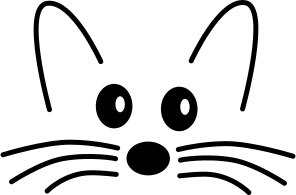
\includegraphics[width=1.4em]{squeak-logo}}}
\newcommand{\dothis}[1]{%
	\medskip
	\noindent\dothisicon
	\ifx#1\empty\else\quad\emph{#1}\fi
	\par\smallskip\nopagebreak}
% NB: To use this in an individual chapter, you must set:
%\graphicspath{{figures/} {../figures/}}
% at the head of the chapter.  Don't forget the final /
%=============================================================
%:Reader hints (hint)
%
% Indicates a non-obvious consequence 
\newcommand{\hint}[1]{\vspace{1ex}\noindent\fbox{\textsc{Astuce}} \emph{#1}}
%=================================================================
% graphics for Morphic handles
\newcommand{\grabHandle}{\raisebox{-0.2ex}{
\includegraphics[width=1em]{blackHandle}}}
\newcommand{\moveHandle}{\raisebox{-0.2ex}{
\includegraphics[width=1em]{moveHandle}}}
\newcommand{\debugHandle}{\raisebox{-0.2ex}{
\includegraphics[width=1em]{debugHandle}}}
% squeak-fr (added for Morphic handles)
\newcommand{\rotateHandle}{\raisebox{-0.2ex}{
\includegraphics[width=1em]{rotateHandle}}}
\newcommand{\viewerHandle}{\raisebox{-0.2ex}{
\includegraphics[width=1em]{viewerHandle}}}
% squeak-fr (add cloverHandle to use \clover in QuickTour.tex as alias
% todo 

%=============================================================
%:Highlighting Important stuff (doublebox)
%
% From Seaside book ...
\newsavebox{\SavedText}
\newlength{\InnerBoxRule}\setlength{\InnerBoxRule}{.75\fboxrule}
\newlength{\OuterBoxRule}\setlength{\OuterBoxRule}{1.5\fboxrule}
\newlength{\BoxSeparation}\setlength{\BoxSeparation}{1.5\fboxrule}
\addtolength{\BoxSeparation}{.5pt}
\newlength{\SaveBoxSep}\setlength{\SaveBoxSep}{2\fboxsep}
%
\newenvironment{doublebox}{\begin{lrbox}{\SavedText}
    \begin{minipage}{.75\textwidth}}
    {\end{minipage}\end{lrbox}\begin{center}
    \setlength{\fboxsep}{\BoxSeparation}\setlength{\fboxrule}{\OuterBoxRule}
    \fbox{\setlength{\fboxsep}{\SaveBoxSep}\setlength{\fboxrule}{\InnerBoxRule}%
      \fbox{\usebox{\SavedText}}}
  \end{center}}
% Use this:
%\newcommand{\important}[1]{\begin{doublebox}#1\end{doublebox}}


\newcommand{\important}[1]{
\noindent\rule{\textwidth}{2pt}\par
\textbf{Important!} #1 \par
\noindent\rule{\textwidth}{2pt}}

\newcommand{\note}[1]{
\noindent\rule{\textwidth}{2pt}\par
\noindent\textbf{Note} #1\par
\noindent\rule{\textwidth}{2pt}}

%=============================================================
%:Section depth
\setcounter{secnumdepth}{2}
%% for this to happen start the file with
%\ifx\wholebook\relax\else
%% $Author$ Martial
% $Date$ Wed Oct 10 13:34:55 CEST 2007
% $Revision$ source: SBE 12715 
% Last Changed Date: 2007-10-08 21:32:45 +0200 (Mon, 08 Oct 2007)
%=============================================================
% NB: documentclass must be set in main document.
% Allows book to be generated in multiple formats.
%=============================================================
%:Packages
%\usepackage[french]{babel}
\usepackage[T1]{fontenc}  %%%%%% really important to get the code directly in the text!
\usepackage{lmodern}
%\usepackage[scaled=0.85]{bookmanx} % needs another scale factor if used with \renewcommand{\sfdefault}{cmbr}
\usepackage{palatino}
%\usepackage[sc]{mathpazo}
%\linespread{1.05}
\usepackage[scaled=0.85]{helvet}
\usepackage{microtype}
\usepackage{graphicx}
\usepackage{theorem}
\usepackage[utf8]{inputenc}
% ON: pdfsync breaks the use of p{width} for tabular columns!
\ifdefined\usepdfsync\usepackage{pdfsync}\fi % Requires texlive 2007
%=============================================================
%:More packages
%Stef should check which ones are used!
%\usepackage{picinpar}
%\usepackage{layout}
%\usepackage{color}
%\definecolor{stefgris}{rgb}{0.85,0.85,0.85}
%\usepackage{enum}
%\usepackage{a4wide}
% \usepackage{fancyhdr}
\usepackage{ifthen}
\usepackage{float}
\usepackage{longtable}
\usepackage{makeidx}
\usepackage[nottoc]{tocbibind}
\usepackage{multicol}
\usepackage{booktabs}	% book-style tables
\usepackage{topcapt}	% enables \topcaption
\usepackage{multirow}
\usepackage{tabularx}
%\usepackage[bottom]{footmisc}
\usepackage{xspace}
\usepackage{alltt}
\usepackage{amssymb,textcomp}
\usepackage[usenames,dvipsnames]{color}
\usepackage{colortbl}
\usepackage[hang]{subfigure}\makeatletter\def\p@subfigure{\thefigure\,}\makeatother
\usepackage{rotating}
\usepackage{enumitem}	% apb: allows more control over tags in enumerations
\usepackage{verbatim}     % for comment environment
\usepackage{varioref}	% for page references that work
\labelformat{footnote}{\thechapter--#1} % to distinguish citations from jurabib
\usepackage{needspace}
\usepackage{isodateo} % enable \isodate
\usepackage[newparttoc]{titlesec}
\usepackage{titletoc}
\usepackage{eurosym}
\usepackage{wrapfig}

\usepackage[
	super,
	citefull=first,
	authorformat={allreversed,and},
	titleformat={commasep,italic}
]{jurabib} % citations as footnotes
\usepackage[
	colorlinks=true,
	linkcolor=black,
	urlcolor=black,
	citecolor=black
]{hyperref}   % should come last

%=============================================================
%:URL style
\makeatletter

\def\url@leostyle{%
  \@ifundefined{selectfont}{\def\UrlFont{\sf}}{\def\UrlFont{\sffamily}}}
% ajouter par Martial pour \traduit (met une dague dans les \doublebox
\def\thempfootnote{\fnsymbol{mpfootnote}}

\makeatother
% Now actually use the newly defined style.
\urlstyle{leo}
%=============================================================
%:Booleans
\newboolean{lulu}
\setboolean{lulu}{false}
\newcommand{\ifluluelse}[2]{\ifthenelse{\boolean{lulu}}{#1}{#2}}
%=============================================================
%:Names
\newcommand{\SUnit}{SUnit\xspace}
\newcommand{\sunit}{SUnit\xspace}
\newcommand{\xUnit}{$x$Unit\xspace}
\newcommand{\JUnit}{JUnit\xspace}
%\newcommand{\XP}{eXtreme Programming\xspace}
\newcommand{\st}{Smalltalk\xspace}
\newcommand{\Squeak}{Squeak\xspace}
\newcommand{\sq}{Squeak\xspace}
\newcommand{\sqmap}{SqueakMap\xspace}
\newcommand{\squeak}{Squeak\xspace}
%\newcommand{\sbe}{\url{scg.unibe.ch/SBE}\xspace}
%\newcommand{\sbe}{\url{squeakbyexample.org}\xspace}
\newcommand{\sbe}{\url{SqueakByExample.org}\xspace}
% squeak-fr: adresse de la version francaise
\newcommand{\spe}{\url{SqueakByExample.org/fr}\xspace}
\newcommand{\sba}{\url{SquareBracketAssociates.org}\xspace}

% squeak-fr: ajout de la \squeakdev pour eviter les problemes de
% changements d'url rencontres dans la VO:
\newcommand{\squeakdev}{\url{www.squeaksource.com/ImageForDevelopers}\xspace} %ou
%\newcommand{\squeakdev}{\url{squeak.ofset.org/squeak-dev}\xspace}

%=============================================================
%:Editorial comment macros
\newcommand{\nnbb}[2]{
    \fbox{\bfseries\sffamily\scriptsize#1}
    {\sf\small$\blacktriangleright$\textit{#2}$\blacktriangleleft$}
   }
\newcommand{\ab}[1]{\nnbb{Andrew}{#1}}
\newcommand{\sd}[1]{\nnbb{St\'{e}f}{#1}}
\newcommand{\md}[1]{\nnbb{Marcus}{#1}}
\newcommand{\on}[1]{\nnbb{Oscar}{#1}}
\newcommand{\damien}[1]{\nnbb{Damien}{#1}}
\newcommand{\lr}[1]{\nnbb{Lukas}{#1}}
\newcommand{\orla}[1]{\nnbb{Orla}{#1}}
%\newcommand{\here}{\nnbb{CONTINUE}{HERE}}
\newcommand{\here}{\nnbb{CONTINUE}{ICI}}

%=============================================================
%:Abbreviation macros
\newcommand{\ie}{\emph{c-\`a-d.}\xspace}
\newcommand{\cad}{\emph{c-\`a-d.}\xspace}
%\newcommand{\eg}{\emph{e.g.},\xspace}
\newcommand{\eg}{\emph{par ex.},\xspace}
\newcommand{\parex}{\emph{par ex.},\xspace}
\newcommand{\etc}{etc\xspace}
%=============================================================
%:Cross reference macros

% [squeak-fr] martial: remarquez les articles devant les noms
\newcommand{\charef}[1]{le chapitre~\ref{cha:#1}\xspace}
% note de martial: utilise dans chapitre Syntax.tex: a redefinir
\newcommand{\charefs}[2]{les chapitres~\ref{cha:#1} et \ref{cha:#2}\xspace}
\newcommand{\secref}[1]{la section~\ref{sec:#1}\xspace}
\newcommand{\figref}[1]{la figure~\ref{fig:#1}\xspace}
\newcommand{\Figref}[1]{La figure~\ref{fig:#1}\xspace}
\newcommand{\appref}[1]{l'annexe~\ref{app:#1}\xspace}
\newcommand{\tabref}[1]{la table~\ref{tab:#1}\xspace}
% defini pour le chapitre Messages.tex
\newcommand{\Tabref}[1]{La table~\ref{tab:#1}\xspace}

% APB: I removed trailing \xspace commands from these macros because
% \xspace mostly doesn't work.  If you want a space after your
% references, type one!
% ON: xspace has always worked just fine for me!  Please leave them in.
%
\newcommand{\ruleref}[1]{\ref{rule:#1}\xspace}
%
\newcommand{\egref}[1]{exemple~\ref{eg:#1}\xspace}
\newcommand{\Egref}[1]{Exemple~\ref{eg:#1}\xspace}
%
\newcommand{\scrref}[1]{script~\ref{scr:#1}\xspace}
\newcommand{\Scrref}[1]{Script~\ref{scr:#1}\xspace}
% t = the
\newcommand{\tscrref}[1]{le script~\ref{scr:#1}\xspace}
\newcommand{\Tscrref}[1]{Le script~\ref{scr:#1}\xspace}
%
\newcommand{\mthref}[1]{m\'ethode~\ref{mth:#1}\xspace}
\newcommand{\mthsref}[1]{m\'ethodes~\ref{mth:#1}\xspace}
\newcommand{\Mthref}[1]{M\'ethode~\ref{mth:#1}\xspace}
\newcommand{\tmthref}[1]{la m\'ethode~\ref{mth:#1}\xspace}
\newcommand{\Tmthref}[1]{La m\'ethode~\ref{mth:#1}\xspace}
%
\newcommand{\clsref}[1]{classe~\ref{cls:#1}\xspace}
\newcommand{\tclsref}[1]{la classe~\ref{cls:#1}\xspace}
\newcommand{\Tclsref}[1]{La classe~\ref{cls:#1}\xspace}
%=============================================================
%:Menu item macro
% for menu items, so we can change our minds on how to print them! (apb)
\definecolor{lightgray}{gray}{0.89}
\newcommand{\menu}[1]{{%
	\setlength{\fboxsep}{0pt}%
	\colorbox{lightgray}{{{\upshape\sffamily\strut \,#1\,}}}}}
% \newcommand{\menu}[1]{{%
% 	\fontfamily{lmr}\selectfont
% 	\upshape\textlangle{\sffamily #1}\textrangle}}
% For submenu items:
\newcommand{\go}{\,$\triangleright$\,}
% \newcommand{\go}{\,$\blacktriangleright$\,}
% For keyboard shortcuts:
%\newcommand{\short}[1]{\mbox{$\langle${\sc CMD}$\rangle$-#1}\xspace}
\newcommand{\short}[1]{\mbox{{\sc cmd}\hspace{0.08em}--\hspace{0.09em}#1}\xspace}
% For buttons:
\newcommand{\button}[1]{{%
	\setlength{\fboxsep}{0pt}%
	\fbox{{\upshape\sffamily\strut \,#1\,}}}}
\newcommand{\toolsflap}{l'onglet \textit{Tools}\xspace}
%=============================================================
%:Reader cues (do this)
%
% Indicate something the reader should try out.
\newcommand{\dothisicon}{\raisebox{-.5ex}{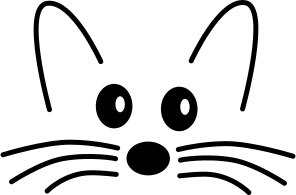
\includegraphics[width=1.4em]{squeak-logo}}}
\newcommand{\dothis}[1]{%
	\medskip
	\noindent\dothisicon
	\ifx#1\empty\else\quad\emph{#1}\fi
	\par\smallskip\nopagebreak}
% NB: To use this in an individual chapter, you must set:
%\graphicspath{{figures/} {../figures/}}
% at the head of the chapter.  Don't forget the final /
%=============================================================
%:Reader hints (hint)
%
% Indicates a non-obvious consequence 
\newcommand{\hint}[1]{\vspace{1ex}\noindent\fbox{\textsc{Astuce}} \emph{#1}}
%=================================================================
% graphics for Morphic handles
\newcommand{\grabHandle}{\raisebox{-0.2ex}{
\includegraphics[width=1em]{blackHandle}}}
\newcommand{\moveHandle}{\raisebox{-0.2ex}{
\includegraphics[width=1em]{moveHandle}}}
\newcommand{\debugHandle}{\raisebox{-0.2ex}{
\includegraphics[width=1em]{debugHandle}}}
% squeak-fr (added for Morphic handles)
\newcommand{\rotateHandle}{\raisebox{-0.2ex}{
\includegraphics[width=1em]{rotateHandle}}}
\newcommand{\viewerHandle}{\raisebox{-0.2ex}{
\includegraphics[width=1em]{viewerHandle}}}
% squeak-fr (add cloverHandle to use \clover in QuickTour.tex as alias
% todo 

%=============================================================
%:Highlighting Important stuff (doublebox)
%
% From Seaside book ...
\newsavebox{\SavedText}
\newlength{\InnerBoxRule}\setlength{\InnerBoxRule}{.75\fboxrule}
\newlength{\OuterBoxRule}\setlength{\OuterBoxRule}{1.5\fboxrule}
\newlength{\BoxSeparation}\setlength{\BoxSeparation}{1.5\fboxrule}
\addtolength{\BoxSeparation}{.5pt}
\newlength{\SaveBoxSep}\setlength{\SaveBoxSep}{2\fboxsep}
%
\newenvironment{doublebox}{\begin{lrbox}{\SavedText}
    \begin{minipage}{.75\textwidth}}
    {\end{minipage}\end{lrbox}\begin{center}
    \setlength{\fboxsep}{\BoxSeparation}\setlength{\fboxrule}{\OuterBoxRule}
    \fbox{\setlength{\fboxsep}{\SaveBoxSep}\setlength{\fboxrule}{\InnerBoxRule}%
      \fbox{\usebox{\SavedText}}}
  \end{center}}
% Use this:
%\newcommand{\important}[1]{\begin{doublebox}#1\end{doublebox}}


\newcommand{\important}[1]{
\noindent\rule{\textwidth}{2pt}\par
\textbf{Important!} #1 \par
\noindent\rule{\textwidth}{2pt}}

\newcommand{\note}[1]{
\noindent\rule{\textwidth}{2pt}\par
\noindent\textbf{Note} #1\par
\noindent\rule{\textwidth}{2pt}}

%=============================================================
%:Section depth
\setcounter{secnumdepth}{2}
%% for this to happen start the file with
%\ifx\wholebook\relax\else
%% $Author$ Martial
% $Date$ Wed Oct 10 13:34:55 CEST 2007
% $Revision$ source: SBE 12715 
% Last Changed Date: 2007-10-08 21:32:45 +0200 (Mon, 08 Oct 2007)
%=============================================================
% NB: documentclass must be set in main document.
% Allows book to be generated in multiple formats.
%=============================================================
%:Packages
%\usepackage[french]{babel}
\usepackage[T1]{fontenc}  %%%%%% really important to get the code directly in the text!
\usepackage{lmodern}
%\usepackage[scaled=0.85]{bookmanx} % needs another scale factor if used with \renewcommand{\sfdefault}{cmbr}
\usepackage{palatino}
%\usepackage[sc]{mathpazo}
%\linespread{1.05}
\usepackage[scaled=0.85]{helvet}
\usepackage{microtype}
\usepackage{graphicx}
\usepackage{theorem}
\usepackage[utf8]{inputenc}
% ON: pdfsync breaks the use of p{width} for tabular columns!
\ifdefined\usepdfsync\usepackage{pdfsync}\fi % Requires texlive 2007
%=============================================================
%:More packages
%Stef should check which ones are used!
%\usepackage{picinpar}
%\usepackage{layout}
%\usepackage{color}
%\definecolor{stefgris}{rgb}{0.85,0.85,0.85}
%\usepackage{enum}
%\usepackage{a4wide}
% \usepackage{fancyhdr}
\usepackage{ifthen}
\usepackage{float}
\usepackage{longtable}
\usepackage{makeidx}
\usepackage[nottoc]{tocbibind}
\usepackage{multicol}
\usepackage{booktabs}	% book-style tables
\usepackage{topcapt}	% enables \topcaption
\usepackage{multirow}
\usepackage{tabularx}
%\usepackage[bottom]{footmisc}
\usepackage{xspace}
\usepackage{alltt}
\usepackage{amssymb,textcomp}
\usepackage[usenames,dvipsnames]{color}
\usepackage{colortbl}
\usepackage[hang]{subfigure}\makeatletter\def\p@subfigure{\thefigure\,}\makeatother
\usepackage{rotating}
\usepackage{enumitem}	% apb: allows more control over tags in enumerations
\usepackage{verbatim}     % for comment environment
\usepackage{varioref}	% for page references that work
\labelformat{footnote}{\thechapter--#1} % to distinguish citations from jurabib
\usepackage{needspace}
\usepackage{isodateo} % enable \isodate
\usepackage[newparttoc]{titlesec}
\usepackage{titletoc}
\usepackage{eurosym}
\usepackage{wrapfig}

\usepackage[
	super,
	citefull=first,
	authorformat={allreversed,and},
	titleformat={commasep,italic}
]{jurabib} % citations as footnotes
\usepackage[
	colorlinks=true,
	linkcolor=black,
	urlcolor=black,
	citecolor=black
]{hyperref}   % should come last

%=============================================================
%:URL style
\makeatletter

\def\url@leostyle{%
  \@ifundefined{selectfont}{\def\UrlFont{\sf}}{\def\UrlFont{\sffamily}}}
% ajouter par Martial pour \traduit (met une dague dans les \doublebox
\def\thempfootnote{\fnsymbol{mpfootnote}}

\makeatother
% Now actually use the newly defined style.
\urlstyle{leo}
%=============================================================
%:Booleans
\newboolean{lulu}
\setboolean{lulu}{false}
\newcommand{\ifluluelse}[2]{\ifthenelse{\boolean{lulu}}{#1}{#2}}
%=============================================================
%:Names
\newcommand{\SUnit}{SUnit\xspace}
\newcommand{\sunit}{SUnit\xspace}
\newcommand{\xUnit}{$x$Unit\xspace}
\newcommand{\JUnit}{JUnit\xspace}
%\newcommand{\XP}{eXtreme Programming\xspace}
\newcommand{\st}{Smalltalk\xspace}
\newcommand{\Squeak}{Squeak\xspace}
\newcommand{\sq}{Squeak\xspace}
\newcommand{\sqmap}{SqueakMap\xspace}
\newcommand{\squeak}{Squeak\xspace}
%\newcommand{\sbe}{\url{scg.unibe.ch/SBE}\xspace}
%\newcommand{\sbe}{\url{squeakbyexample.org}\xspace}
\newcommand{\sbe}{\url{SqueakByExample.org}\xspace}
% squeak-fr: adresse de la version francaise
\newcommand{\spe}{\url{SqueakByExample.org/fr}\xspace}
\newcommand{\sba}{\url{SquareBracketAssociates.org}\xspace}

% squeak-fr: ajout de la \squeakdev pour eviter les problemes de
% changements d'url rencontres dans la VO:
\newcommand{\squeakdev}{\url{www.squeaksource.com/ImageForDevelopers}\xspace} %ou
%\newcommand{\squeakdev}{\url{squeak.ofset.org/squeak-dev}\xspace}

%=============================================================
%:Editorial comment macros
\newcommand{\nnbb}[2]{
    \fbox{\bfseries\sffamily\scriptsize#1}
    {\sf\small$\blacktriangleright$\textit{#2}$\blacktriangleleft$}
   }
\newcommand{\ab}[1]{\nnbb{Andrew}{#1}}
\newcommand{\sd}[1]{\nnbb{St\'{e}f}{#1}}
\newcommand{\md}[1]{\nnbb{Marcus}{#1}}
\newcommand{\on}[1]{\nnbb{Oscar}{#1}}
\newcommand{\damien}[1]{\nnbb{Damien}{#1}}
\newcommand{\lr}[1]{\nnbb{Lukas}{#1}}
\newcommand{\orla}[1]{\nnbb{Orla}{#1}}
%\newcommand{\here}{\nnbb{CONTINUE}{HERE}}
\newcommand{\here}{\nnbb{CONTINUE}{ICI}}

%=============================================================
%:Abbreviation macros
\newcommand{\ie}{\emph{c-\`a-d.}\xspace}
\newcommand{\cad}{\emph{c-\`a-d.}\xspace}
%\newcommand{\eg}{\emph{e.g.},\xspace}
\newcommand{\eg}{\emph{par ex.},\xspace}
\newcommand{\parex}{\emph{par ex.},\xspace}
\newcommand{\etc}{etc\xspace}
%=============================================================
%:Cross reference macros

% [squeak-fr] martial: remarquez les articles devant les noms
\newcommand{\charef}[1]{le chapitre~\ref{cha:#1}\xspace}
% note de martial: utilise dans chapitre Syntax.tex: a redefinir
\newcommand{\charefs}[2]{les chapitres~\ref{cha:#1} et \ref{cha:#2}\xspace}
\newcommand{\secref}[1]{la section~\ref{sec:#1}\xspace}
\newcommand{\figref}[1]{la figure~\ref{fig:#1}\xspace}
\newcommand{\Figref}[1]{La figure~\ref{fig:#1}\xspace}
\newcommand{\appref}[1]{l'annexe~\ref{app:#1}\xspace}
\newcommand{\tabref}[1]{la table~\ref{tab:#1}\xspace}
% defini pour le chapitre Messages.tex
\newcommand{\Tabref}[1]{La table~\ref{tab:#1}\xspace}

% APB: I removed trailing \xspace commands from these macros because
% \xspace mostly doesn't work.  If you want a space after your
% references, type one!
% ON: xspace has always worked just fine for me!  Please leave them in.
%
\newcommand{\ruleref}[1]{\ref{rule:#1}\xspace}
%
\newcommand{\egref}[1]{exemple~\ref{eg:#1}\xspace}
\newcommand{\Egref}[1]{Exemple~\ref{eg:#1}\xspace}
%
\newcommand{\scrref}[1]{script~\ref{scr:#1}\xspace}
\newcommand{\Scrref}[1]{Script~\ref{scr:#1}\xspace}
% t = the
\newcommand{\tscrref}[1]{le script~\ref{scr:#1}\xspace}
\newcommand{\Tscrref}[1]{Le script~\ref{scr:#1}\xspace}
%
\newcommand{\mthref}[1]{m\'ethode~\ref{mth:#1}\xspace}
\newcommand{\mthsref}[1]{m\'ethodes~\ref{mth:#1}\xspace}
\newcommand{\Mthref}[1]{M\'ethode~\ref{mth:#1}\xspace}
\newcommand{\tmthref}[1]{la m\'ethode~\ref{mth:#1}\xspace}
\newcommand{\Tmthref}[1]{La m\'ethode~\ref{mth:#1}\xspace}
%
\newcommand{\clsref}[1]{classe~\ref{cls:#1}\xspace}
\newcommand{\tclsref}[1]{la classe~\ref{cls:#1}\xspace}
\newcommand{\Tclsref}[1]{La classe~\ref{cls:#1}\xspace}
%=============================================================
%:Menu item macro
% for menu items, so we can change our minds on how to print them! (apb)
\definecolor{lightgray}{gray}{0.89}
\newcommand{\menu}[1]{{%
	\setlength{\fboxsep}{0pt}%
	\colorbox{lightgray}{{{\upshape\sffamily\strut \,#1\,}}}}}
% \newcommand{\menu}[1]{{%
% 	\fontfamily{lmr}\selectfont
% 	\upshape\textlangle{\sffamily #1}\textrangle}}
% For submenu items:
\newcommand{\go}{\,$\triangleright$\,}
% \newcommand{\go}{\,$\blacktriangleright$\,}
% For keyboard shortcuts:
%\newcommand{\short}[1]{\mbox{$\langle${\sc CMD}$\rangle$-#1}\xspace}
\newcommand{\short}[1]{\mbox{{\sc cmd}\hspace{0.08em}--\hspace{0.09em}#1}\xspace}
% For buttons:
\newcommand{\button}[1]{{%
	\setlength{\fboxsep}{0pt}%
	\fbox{{\upshape\sffamily\strut \,#1\,}}}}
\newcommand{\toolsflap}{l'onglet \textit{Tools}\xspace}
%=============================================================
%:Reader cues (do this)
%
% Indicate something the reader should try out.
\newcommand{\dothisicon}{\raisebox{-.5ex}{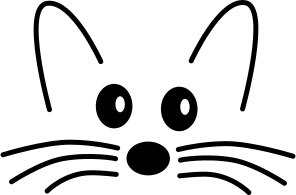
\includegraphics[width=1.4em]{squeak-logo}}}
\newcommand{\dothis}[1]{%
	\medskip
	\noindent\dothisicon
	\ifx#1\empty\else\quad\emph{#1}\fi
	\par\smallskip\nopagebreak}
% NB: To use this in an individual chapter, you must set:
%\graphicspath{{figures/} {../figures/}}
% at the head of the chapter.  Don't forget the final /
%=============================================================
%:Reader hints (hint)
%
% Indicates a non-obvious consequence 
\newcommand{\hint}[1]{\vspace{1ex}\noindent\fbox{\textsc{Astuce}} \emph{#1}}
%=================================================================
% graphics for Morphic handles
\newcommand{\grabHandle}{\raisebox{-0.2ex}{
\includegraphics[width=1em]{blackHandle}}}
\newcommand{\moveHandle}{\raisebox{-0.2ex}{
\includegraphics[width=1em]{moveHandle}}}
\newcommand{\debugHandle}{\raisebox{-0.2ex}{
\includegraphics[width=1em]{debugHandle}}}
% squeak-fr (added for Morphic handles)
\newcommand{\rotateHandle}{\raisebox{-0.2ex}{
\includegraphics[width=1em]{rotateHandle}}}
\newcommand{\viewerHandle}{\raisebox{-0.2ex}{
\includegraphics[width=1em]{viewerHandle}}}
% squeak-fr (add cloverHandle to use \clover in QuickTour.tex as alias
% todo 

%=============================================================
%:Highlighting Important stuff (doublebox)
%
% From Seaside book ...
\newsavebox{\SavedText}
\newlength{\InnerBoxRule}\setlength{\InnerBoxRule}{.75\fboxrule}
\newlength{\OuterBoxRule}\setlength{\OuterBoxRule}{1.5\fboxrule}
\newlength{\BoxSeparation}\setlength{\BoxSeparation}{1.5\fboxrule}
\addtolength{\BoxSeparation}{.5pt}
\newlength{\SaveBoxSep}\setlength{\SaveBoxSep}{2\fboxsep}
%
\newenvironment{doublebox}{\begin{lrbox}{\SavedText}
    \begin{minipage}{.75\textwidth}}
    {\end{minipage}\end{lrbox}\begin{center}
    \setlength{\fboxsep}{\BoxSeparation}\setlength{\fboxrule}{\OuterBoxRule}
    \fbox{\setlength{\fboxsep}{\SaveBoxSep}\setlength{\fboxrule}{\InnerBoxRule}%
      \fbox{\usebox{\SavedText}}}
  \end{center}}
% Use this:
%\newcommand{\important}[1]{\begin{doublebox}#1\end{doublebox}}


\newcommand{\important}[1]{
\noindent\rule{\textwidth}{2pt}\par
\textbf{Important!} #1 \par
\noindent\rule{\textwidth}{2pt}}

\newcommand{\note}[1]{
\noindent\rule{\textwidth}{2pt}\par
\noindent\textbf{Note} #1\par
\noindent\rule{\textwidth}{2pt}}

%=============================================================
%:Section depth
\setcounter{secnumdepth}{2}
%% for this to happen start the file with
%\ifx\wholebook\relax\else
%\input{../common.tex}
%\begin{document}
%\fi
% and terminate by
% \ifx\wholebook\relax\else\end{document}\fi

\DeclareGraphicsExtensions{.pdf, .jpg, .png}
%=============================================================
%:PDF setup
\hypersetup{
%   a4paper,
%   pdfstartview=FitV,
%   colorlinks,
%   linkcolor=darkblue,
%   citecolor=darkblue,
%   pdftitle={Squeak by Example},
pdftitle={Squeak par l'exemple},
   pdfauthor={Andrew Black, St\'ephane Ducasse,	Oscar Nierstrasz,
Damien Pollet},
   pdfkeywords={Smalltalk, Squeak, Programmation Orient\'ee Objet},
pdfsubject={Informatique, Computer Science}
}
%=============================================================
%:Page layout and appearance
%
% \renewcommand{\headrulewidth}{0pt}
\renewcommand{\chaptermark}[1]{\markboth{#1}{}}
\renewcommand{\sectionmark}[1]{\markright{\thesection\ #1}}
\renewpagestyle{plain}[\small\itshape]{%
	\setheadrule{0pt}%
	\sethead[][][]{}{}{}%
	\setfoot[][][]{}{}{}}
\renewpagestyle{headings}[\small\itshape]{%
	\setheadrule{0pt}%
	\setmarks{chapter}{section}%
	\sethead[\thepage][][\chaptertitle]{\sectiontitle}{}{\thepage}%
	\setfoot[][][]{}{}{}}
% pagestyle for tableofcontents + index (martial: 2008/04/23)
\newpagestyle{newheadings}[\small\itshape]{%
	\setheadrule{0pt}%
	\setmarks{chapter}{section}%
	\sethead[\thepage][][\chaptertitle]{\chaptertitle}{}{\thepage}%
	\setfoot[][][]{}{}{}}
%=============================================================
%:Title section setup and TOC numbering depth
\setcounter{secnumdepth}{1}
\setcounter{tocdepth}{1}
\titleformat{\part}[display]{\centering}{\huge\partname\ \thepart}{1em}{\Huge\textbf}[]
\titleformat{\chapter}[display]{}{\huge\chaptertitlename\ \thechapter}{1em}{\Huge\raggedright\textbf}[]
\titlecontents{part}[3pc]{%
		\pagebreak[2]\addvspace{1em plus.4em minus.2em}%
		\leavevmode\large\bfseries}
	{\contentslabel{3pc}}{\hspace*{-3pc}}
	{}[\nopagebreak]
\titlecontents{chapter}[3pc]{%
		\pagebreak[0]\addvspace{1em plus.2em minus.2em}%
		\leavevmode\bfseries}
	{\contentslabel{3pc}}{}
	{\hfill\contentspage}[\nopagebreak]
\dottedcontents{section}[3pc]{}{3pc}{1pc}
\dottedcontents{subsection}[3pc]{}{0pc}{1pc}
% \dottedcontents{subsection}[4.5em]{}{0pt}{1pc}
% Make \cleardoublepage insert really blank pages http://www.tex.ac.uk/cgi-bin/texfaq2html?label=reallyblank
\let\origdoublepage\cleardoublepage
\newcommand{\clearemptydoublepage}{%
  \clearpage
  {\pagestyle{empty}\origdoublepage}}
\let\cleardoublepage\clearemptydoublepage % see http://www.tex.ac.uk/cgi-bin/texfaq2html?label=patch
%=============================================================
%:FAQ macros (for FAQ chapter)
\newtheorem{faq}{FAQ}
\newcommand{\answer}{\paragraph{R\'eponse}\ }
%=============================================================
%:Listings package configuration
\usepackage{listings}
\newcommand{\caret}{\makebox{\raisebox{0.4ex}{\footnotesize{$\wedge$}}}}
\lstdefinelanguage{Smalltalk}{
%  morekeywords={self,super,true,false,nil,thisContext}, % This is overkill
  morestring=[d]',
  morecomment=[s]{"}{"},
  alsoletter={\#:},
  escapechar={!},
  escapebegin=\itshape, % comment-like by default (Martial 11/2007)
  literate=
    {BANG}{!}1
    {UNDERSCORE}{\_}1
    {\\st}{Smalltalk}9 % convenience -- in case \st occurs in code
    % {'}{{\textquotesingle}}1 % replaced by upquote=true in \lstset
    {_}{{$\leftarrow$}}1
    {>>>}{{\sep}}1
    {^}{{$\uparrow$}}1
    {~}{{$\sim$}}1
    {-}{{\sf -\hspace{-0.13em}-}}1  % the goal is to make - the same width as +
    {+}{\raisebox{0.08ex}{+}}1		% and to raise + off the baseline to match -
    {-->}{{\quad$\longrightarrow$\quad}}3
	, % Don't forget the comma at the end!
  tabsize=4
}[keywords,comments,strings]
% ajout pour les échappements dans les codes
% indispensable pour mettre le code en emphase (cf. Model.tex) 
\newcommand{\codeify}[1]{\NoAutoSpaceBeforeFDP#1\AutoSpaceBeforeFDP}
\newcommand{\normcomment}[1]{\emph{#1}} %cf. Streams
\newcommand{\normcode}[1]{\emph{\codeify{#1}}} %cf. Streams
\newcommand{\emcode}[1]{\textbf{\normcode{#1}}} % Martial 11/2007
\lstset{language=Smalltalk,
	basicstyle=\sffamily,
	keywordstyle=\color{black}\bfseries,
	% stringstyle=\ttfamily, % Ugly! do we really want this? -- on
	%commentstyle=\itshape,
	mathescape=true,
	showstringspaces=false,
	keepspaces=true,
	breaklines=true,
	breakautoindent=true,
	lineskip={-1pt}, % Ugly hack
	upquote=true, % straight quote; requires textcomp package
	columns=fullflexible} % no fixed width fonts
% In-line code (literal)
% Normally use this for all in-line code:
\newcommand{\ct}{\lstinline[mathescape=false,basicstyle={\sffamily\upshape}]}
% apb 2007.8.28 added the \upshape declaration to avoid getting italicized code in \dothis{ } sections.
% In-line code (latex enabled)
% Use this only in special situations where \ct does not work
% (within section headings ...):

% [squeak-fr] Modification de \lct suivant les indications de Martial Boniou
\newcommand{\lct}[1]{\textsf{\textup{\NoAutoSpaceBeforeFDP #1
\AutoSpaceBeforeFDP}}} %\xspace

% Use these for system categories and protocols:
\newcommand{\scat}[1]{\emph{\textsf{#1}}\xspace}
\newcommand{\pkg}[1]{\emph{\textsf{#1}}\xspace}
\newcommand{\prot}[1]{\emph{\textsf{#1}}\xspace}
% Code environments
% NB: the arg is for tests
% Only code and example environments may be tests
\lstnewenvironment{code}[1]{%
	\lstset{%
		frame=lines,
		mathescape=false
	}
}{}
\def\ignoredollar#1{}
%=============================================================
%:Code environments (method, script ...)
% NB: the third arg is for tests
% Only code and example environments may be tests
\lstnewenvironment{example}[3][defaultlabel]{%
	\renewcommand{\lstlistingname}{Exemple}%
	\lstset{
		frame=lines,
		mathescape=false,
		caption={\emph{#2}},
		label={eg:#1}
	}
}{}
\lstnewenvironment{script}[2][defaultlabel]{%
\renewcommand{\lstlistingname}{Script}%
	\lstset{
		frame=lines,
		mathescape=false,
		name={Script},
		caption={\emph{#2}},
		label={scr:#1}
	}
}{}
%I could not find a way yo get the Experiment #numb followed by the caption in a black box
%\colorbox{black}{\makebox[\textwidth]{  \color{white} {\large {\bfseries Experiment 3-1 (crear i moure un robot)}} }}
\lstnewenvironment{experiment}[2][defaultlabel]{%
%\noindent\rule{\textwidth}{2pt}\vspace{-0.8cm}
\renewcommand{\lstlistingname}{Experiment}%
	\lstset{
		frame=none,
		rulecolor=\color{black},
		mathescape=false,
		name={Experiment},
		caption={\emph{#2}},
		label={scr:#1}
	}
}{%\vspace{-0.5cm}\noindent\rule{\textwidth}{2pt}
}

\lstnewenvironment{method}[2][defaultlabel]{%
	\renewcommand{\lstlistingname}{Method}%
	\lstset{
		frame=lines,
		mathescape=false,
		name={M\'ethode},
		caption={\emph{#2}},
		label={mth:#1}
	}
}{}
\lstnewenvironment{methods}[2][defaultlabel]{% just for multiple methods at once
	\renewcommand{\lstlistingname}{Methods}%
	\lstset{
		frame=lines,
		mathescape=false,
		name={M\'ethode},
		caption={\emph{#2}},
		label={mth:#1}
	}
}{}
\lstnewenvironment{numMethod}[2][defaultlabel]{%
	\renewcommand{\lstlistingname}{Method}%
	\lstset{
		numbers=left,
		numberstyle={\tiny\sffamily},
		frame=lines,
		mathescape=false,
		name={M\'ethode},
		caption={\emph{#2}},
		label={mth:#1}
	}
}{}
% \lstnewenvironment{classdef}[2][defaultlabel]{%
% 	\renewcommand{\lstlistingname}{Classe}%
% 	\lstset{
% 		frame=lines,
% 		mathescape=false,
% 		name={Classe},
% 		caption={\emph{#2}},
% 		label={cls:#1}
% 	}
% }{}

%%%%%%%%%%%%%%%%%%%%%%%%%%%%%%%%%%%%%%%%%%%%%%%%%%%%%%%%%%%%%%%%%%%%%%%%%%%%%%%%%%%%%%%%%%%%%%%%%
%%From the original book latex template
%%%%%%%%%%%%%%%%%%%%%%%%%%%%%%%%%%%%%%%%%%%%%%%%%%%%%%%%%%%%%%%%%%%%%%%%%%%%%%%%%%%%%%%%%%%%%%%%%
\theoremstyle{break}
{\theorembodyfont{\rmfamily}\theoremstyle{break}
\newtheorem{privScript}{Script}[chapter]
%\newtheorem{privMethod}{Method}[chapter]
\newtheorem{privExercise}{Experiment}[chapter]}

% \theoremstyle{break}
% {\theorembodyfont{\rmfamily} \newtheorem{privMethod}{Method}[chapter]}

%class
\theoremstyle{break}
{\theorembodyfont{\rmfamily} \newtheorem{privClassDef}{Class}[chapter]}

%important
\theoremstyle{break}
{\theorembodyfont{\rmfamily} \newtheorem{privTemplate}{Important Messages}[chapter]}

% experiment
\newenvironment{exercise}
    {\begin{privExercise}\mbox{}\\}
    {\end{privExercise}}


%%% for figure
\newsavebox{\ScriptFigure}
\newlength{\ScriptWidth}
\newlength{\FigureWidth}

%%%%%%%%%%%%%%%%%%%%%%%%%%%%%%%%%%%%%%%%%%%%%%%%%%%%%%%%%%%%%%%%%%%%%%%%%%%%%%%%
\newenvironment{scriptfig}[3][0.6]
   {\setlength{\ScriptWidth}{\linewidth*\real{#1}}%
   \setlength{\FigureWidth}{\linewidth-(\linewidth*\real{#1})}%
   \savebox{\ScriptFigure}%
	{\parbox{\FigureWidth}{\includegraphics[width=0.98\FigureWidth]{#2}}}%
   \par\noindent\begin{minipage}{\linewidth}\hrule\vskip 0.2cm\begin{minipage}[c]{\ScriptWidth}%
   \begin{stefscript}[{\em #3}]\begin{alltt}\sffamily}
   {\end{alltt}\end{stefscript}\end{minipage}\hfill
   \usebox{\ScriptFigure}
   \vskip 1ex\hrule\end{minipage}\vskip 1ex\par}

%%%%%%%%%%%%%%%%%%%%%%%%%%%%%%%%%%%%%%%%%%%%%%%%%%%%%%%%%%%%%%%%%%%%%%%%%%%%%%%%
%% to be able to specify the complete set of values for includegraphics
%% may be will be changed but not the interface
\newenvironment{scriptfigwithsize}[3][0.6]
   {\setlength{\ScriptWidth}{\linewidth*\real{#1}}%
   \setlength{\FigureWidth}{\linewidth-(\linewidth*\real{#1})}%
   \savebox{\ScriptFigure}{\parbox{\FigureWidth}{\raggedleft{#2}}}%
   \par\noindent\begin{minipage}{\linewidth}\hrule\vskip 0.3cm\begin{minipage}[c]{\ScriptWidth}%
   \begin{stefscript}[{\em #3}]\begin{alltt}\sffamily}
   {\end{alltt}\end{stefscript}\end{minipage}\hfill
   \usebox{\ScriptFigure}
   \vskip 1ex\hrule\end{minipage}\vskip 1ex\par}

% \newenvironment{methodfig}[2][0.6]
%    {\setlength{\ScriptWidth}{\linewidth*\real{#1}}%
%    \setlength{\FigureWidth}{\linewidth-(\linewidth*\real{#1})}%
%    \savebox{\ScriptFigure}{\parbox{\FigureWidth}{\includegraphics[width=.98\FigureWidth]{#2}}}%
%    \par\noindent\rule{\linewidth}{1mm}
%    \\[-0.3cm]\noindent\rule{\linewidth}{0.1mm}
%    \noindent\begin{minipage}[c]{\ScriptWidth}\begin{privMethod}\begin{alltt}\sffamily}
%    {\end{alltt}\end{privMethod}\end{minipage}\hfill
%    \usebox{\ScriptFigure} \vskip 1ex\hrule\vskip 1ex\par}

% \newenvironment{method}
% {\par\noindent\begin{minipage}{\linewidth}\vspace{0.2cm}\begin{privMethod}\begin{nminipage}\vspace{-0.2cm}\rule{\linewidth}{1mm}\\[-0.6cm]\rule{\linewidth}{0.1mm}\end{nminipage}\hspace*{\scriptindent}\codesize\begin{nalltt}\vspace{-0.2cm}}
% {\end{nalltt}\normalsize\vspace{-0.1cm}\hrule\end{privMethod}\vspace{0.2cm}\end{minipage}}


% \newenvironment{classdef}
% {\par\noindent\begin{minipage}{\linewidth}\vspace{0.2cm}\begin{privClassDef}\begin{nminipage}\vspace{-0.2cm}\rule{\linewidth}{1mm}\\[-0.6cm]\rule{\linewidth}{0.1mm}\end{nminipage}\hspace*{\scriptindent}\codesize\begin{nalltt}\vspace{-0.2cm}}
% {\end{nalltt}\normalsize\vspace{-0.1cm}\hrule\end{privClassDef}\vspace{0.2cm}\end{minipage}}


% \newenvironment{template}
% {\par\noindent\begin{minipage}{\linewidth}\vspace{0.3cm}\begin{privTemplate}\begin{nminipage}\vspace{-0.4cm}\rule{\linewidth}{0.1mm}\end{nminipage}\hspace*{\scriptindent}\begin{nalltt}\vspace{-0.7cm}}
% {\end{nalltt}\vspace{-0.1cm}\hrule\end{privTemplate}\end{minipage}\vspace{0.3cm}}

\newenvironment{exofig}[2][0.7]
   {\setlength{\ScriptWidth}{\linewidth*\real{#1}}
   \setlength{\FigureWidth}{\linewidth-(\linewidth*\real{#1})}
   \savebox{\ScriptFigure}{\parbox{\FigureWidth}{\raggedleft{\includegraphics[width=.98\FigureWidth]{#2}}}}
   \par\noindent\begin{minipage}{\linewidth}\hrule\vskip 0.3cm\begin{minipage}[c]{\ScriptWidth}%
   \begin{privExercise}}
   {\end{privExercise}\end{minipage}\hfill
   \usebox{\ScriptFigure}
   \vskip 1ex\hrule\end{minipage}\vskip 1ex\par}

\newenvironment{exofigwithsize}[2][0.7]
   {\setlength{\ScriptWidth}{\linewidth*\real{#1}}
   \setlength{\FigureWidth}{\linewidth-(\linewidth*\real{#1})}
   \savebox{\ScriptFigure}{\parbox{\FigureWidth}{\raggedleft{#2}}}
   \par\noindent\begin{minipage}{\linewidth}\hrule\vskip 0.3cm\begin{minipage}[c]{\ScriptWidth}%
   \begin{privExercise}}
   {\end{privExercise}\end{minipage}\hfill\usebox{\ScriptFigure}
   \vskip 1ex\hrule\end{minipage}\vskip 1ex\par}

\newenvironment{exofigwithsizeandtitle}[3][0.7]
   {\setlength{\ScriptWidth}{\linewidth*\real{#1}}
   \setlength{\FigureWidth}{\linewidth-(\linewidth*\real{#1})}
   \savebox{\ScriptFigure}{\parbox{\FigureWidth}{\raggedleft{#2}}}
   \vskip 0.3cm\par\noindent\begin{minipage}{\linewidth}\hrule\vskip 0.1cm\begin{minipage}[c]{\ScriptWidth}%
   \begin{privExercise}[\em{#3}]}
   {\end{privExercise}\end{minipage}\hfill\usebox{\ScriptFigure}
   \vskip 1ex\hrule\end{minipage}\vskip 1ex\par}

\newenvironment{exofigwithtitle}[3][0.7]
   {\setlength{\ScriptWidth}{\linewidth*\real{#1}}
   \setlength{\FigureWidth}{\linewidth-(\linewidth*\real{#1})}
   \savebox{\ScriptFigure}{\parbox{\FigureWidth}{\raggedleft{\includegraphics[width=.98\FigureWidth]{#2}}}}
   \par\noindent\begin{minipage}{\linewidth}\hrule\vskip 0.3cm\begin{minipage}[c]{\ScriptWidth}%
   \begin{privExercise}[\em{#3}]}
   {\end{privExercise}\end{minipage}\hfill
   \usebox{\ScriptFigure}
   \vskip 1ex\hrule\end{minipage}\vskip 1ex\par}


\newenvironment{exonofigwithtitle}[3][0.7]
   {\setlength{\ScriptWidth}{\linewidth*\real{#1}}
   \setlength{\FigureWidth}{\linewidth-(\linewidth*\real{#1})}
   \savebox{\ScriptFigure}{\parbox{\FigureWidth}{\raggedleft{\includegraphics[width=.98\FigureWidth]{#2}}}}
   \par\noindent\begin{minipage}{\linewidth}\hrule\vskip 0.3cm\begin{minipage}[c]{\ScriptWidth}%
   \begin{privExercise}[\em{#3}]}
   {\end{privExercise}\end{minipage}\hfill
   \usebox{\ScriptFigure}
   \vskip 1ex\hrule\end{minipage}\vskip 1ex\par}

\newenvironment{exonofig}
   {\par\noindent\begin{minipage}[t]{\linewidth}\noindent\begin{privExercise}}
   {\end{privExercise}\end{minipage}\vspace{0.5cm}\par}

\newenvironment{exonofigtitle}[1]
   {\par\noindent\begin{minipage}[t]{\linewidth}\noindent\begin{privExercise}[\em{#1}]}
   {\end{privExercise}\end{minipage}\vspace{0.5cm}\par}
		
% \newenvironment{solfig}[3][0.5]
%    {\setlength{\ScriptWidth}{\linewidth*\real{#1}}
%    \setlength{\FigureWidth}{\linewidth-\linewidth*\real{#1}}
%    \savebox{\ScriptFigure}{\parbox{\FigureWidth}{\includegraphics[width=.9\linewidth]{#2}}}
%    \par\noindent\vskip 1ex\hrule\vskip 1ex\begin{minipage}[t]{\ScriptWidth}
%    {\bf Solution #3} \begin{alltt}\sffamily}
%    {\end{alltt}\end{minipage}\hfill
%    \usebox{\ScriptFigure}
%    \vskip 1ex\hrule\vskip 1ex\par}
% 
% \newenvironment{solnofig}[1]
%    {\par\noindent\vskip 1ex\hrule\vskip 1ex\begin{minipage}[t]{\ScriptWidth}
%    {\bf Solution #1} \begin{alltt}\sffamily}
%    {\end{alltt}\end{minipage}\hfill
%    \vskip 1ex\hrule\vskip 1ex\par}
% 
% \newenvironment{exoscript}[3][0.5]
%    {\setlength{\ScriptWidth}{\linewidth*\real{#1}}
%     \setlength{\FigureWidth}{\linewidth-\linewidth*\real{#1}}
%     \savebox{\ScriptFigure}{\begin{minipage}\begin{alltt}\sffamily#3\end{alltt}\end{minipage}}
%     \par\noindent\vskip 1ex\hrule\vskip 1ex\begin{minipage}[t]{\ScriptWidth}
%     \begin{privExercise}}
%     {\end{privExercise}\end{minipage}\hfill
%     \usebox{\ScriptFigure}
% \vskip 1ex\hrule\vskip 1ex\par}


%%%%%%%%%%%%%%%%%%%%%%%%%%%%%%%%%%%%%%%%%%%%%%%%%%%%%%%%%%%%%%%%
%% Define the indentation from which the code script starts
%\newlength{\scriptindent}
%\setlength{\scriptindent}{.3cm}
%%%%%%%%%%%%%%%%%%%%%%%%%%%%%%%%%%%%%%%%%%%%%%%%%%%%%%%%%%%%%%%%
%% Method presentation 
%\newlength{\methodindent}
%\newlength{\methodwordlength}
%\newlength{\aftermethod}
%\setlength{\methodindent}{0.2cm}
%\settowidth{\methodwordlength}{\ M\'ethode\ }

%%%%%%%%%%%%%%%%%%%%%%%%%%%%%%%%%%%%%%%%%%%%%%%%%%%%%%%%%%%%%%%%
\theoremstyle{break}
{\theorembodyfont{\rmfamily} \newtheorem{fonction}{Script}[chapter]}

\newsavebox{\fminibox}
\newlength{\fminilength}
% Fait un truc encadre
\newenvironment{fminipage}[1][\linewidth]
  {\setlength{\fminilength}{#1-2\fboxsep-2\fboxrule}
        \begin{lrbox}{\fminibox}\begin{minipage}{\fminilength}}
  { \end{minipage}\end{lrbox}\noindent\fbox{\usebox{\fminibox}}}

% Pareil mais pas encadre (a utiliser pour ne pas couper une fonction en 2)
\newenvironment{nminipage}[1][\linewidth]
  {\setlength{\fminilength}{#1}
        \begin{lrbox}{\fminibox}\begin{minipage}{\fminilength}}
  { \end{minipage}\end{lrbox}\noindent\mbox{\usebox{\fminibox}}}

% Un alltt encadre
\newenvironment{falltt}
  {\vspace*{0.3cm}\begin{fminipage}\begin{alltt}\ttfamily}
  {\end{alltt}\end{fminipage}\vspace*{0.3cm}}

% Un alltt pas encadre
\newenvironment{nalltt}
  {\vspace*{0.3cm}\begin{nminipage}\begin{alltt}\sffamily}
  {\end{alltt}\end{nminipage}\vspace*{0.3cm}}

% Une fonction encadree
\newenvironment{ffonction}[1]
  {\begin{fonction}[#1]\begin{fminipage}\begin{alltt}\ttfamily\rule{\linewidth}{0.5pt}}
{\end{alltt}\end{fminipage}\end{fonction}}


\theoremstyle{break}
{\theorembodyfont{\rmfamily} \newtheorem{stefscript}{Script}[chapter]}

\theoremstyle{break}
{\theorembodyfont{\rmfamily} \newtheorem{exampleScript}{Examples}[chapter]}


%%Not used
\newenvironment{ncscript}[1]
{\vspace{-0.5cm}\begin{stefscript}[#1]\begin{nalltt}\rule{\linewidth}{1.5pt}\vspace{-0.1cm}
\hspace*{\scriptindent}\begin{nalltt}}
{\end{nalltt}\vspace{-0.5cm}\hrule\end{nalltt}\end{stefscript}\vspace{-0.5cm}}
%%Not used
\newenvironment{soluscript}[1]
{\begin{nalltt}\textbf{Solution du script : #1.}\\
\rule{\linewidth}{1.5pt}
\hspace*{\scriptindent}\begin{nalltt}}
{\end{nalltt}\vspace{-0.5cm}\hrule\end{nalltt}\vspace{-0.5cm}\\}




\newenvironment{scriptwithtitle}[1]
{\vspace{-0.3cm}\begin{stefscript}[{\em #1}]\begin{nalltt}\rule{\linewidth}{1.5pt}\vspace{-0.3cm}\hspace*{\scriptindent}\begin{nalltt}\codesize}
{\normalsize\end{nalltt}\vspace{-0.2cm}\hrule\end{nalltt}\end{stefscript}\vspace{-0.5cm}}

\newenvironment{scriptwithouttitle}
{\vspace{-0.5cm}\begin{stefscript}\codesize\begin{nalltt}\rule{\linewidth}{1.5pt}\vspace{-0.1cm}
\hspace*{\scriptindent}\begin{nalltt}}
{\end{nalltt}\vspace{-0.5cm}\hrule\end{nalltt}\normalsize\end{stefscript}\vspace{-0.5cm}}

% \newenvironment{example}
% {\vspace{-0.5cm}\begin{exampleScript}\codesize\begin{nalltt}\rule{\linewidth}{1.5pt}\vspace{-0.1cm}\hspace*{\scriptindent}\begin{nalltt}}
% {\end{nalltt}\vspace{-0.2cm}\hrule\end{nalltt}\normalsize\end{exampleScript}\vspace{-0.5cm}}




























%=============================================================
%:Reserving space
% Usually need one more line than the actual lines of code
\newcommand{\needlines}[1]{\Needspace{#1\baselineskip}}
%=============================================================
%:Indexing macros
% Macros ending with "ind" generate text as well as an index entry
% Macros ending with "index" *only* generate an index entry
\newcommand{\ind}[1]{\index{#1}#1\xspace} % plain text
\newcommand{\subind}[2]{\index{#1!#2}#2\xspace} % show #2, subindex inder #1
\newcommand{\emphind}[1]{\index{#1}\emph{#1}\xspace} % emph #1
\newcommand{\emphsubind}[2]{\index{#1!#2}\emph{#2}\xspace} % show emph #2, subindex inder #1
\newcommand{\scatind}[1]{\index{#1@\textsf{#1} (cat\'egorie)}\scat{#1}} % category
\newcommand{\protind}[1]{\index{#1@\textsf{#1} (protocole)}\prot{#1}} % protocol
% \newcommand{\clsind}[1]{\index{#1@\textsf{#1} (class)}\ct{#1}\xspace}
\newcommand{\clsind}[1]{\index{#1!\#@(classe)}\ct{#1}\xspace} % class
\newcommand{\cvind}[1]{\index{#1@\textsf{#1} (variable de classe)}\ct{#1}\xspace} % class var
\newcommand{\glbind}[1]{\index{#1@\textsf{#1} (globale)}\ct{#1}\xspace} % global
\newcommand{\patind}[1]{\index{#1@#1 (patron)}\ct{#1}\xspace} % pattern
\newcommand{\pvind}[1]{\index{#1@\textsf{#1} (pseudo-variable)}\ct{#1}\xspace} % pseudo variable
% [squeak - fr]Martial: I found the following cleaner (should be
% merged in SBE for self and super)
\newcommand{\subpvindex}[2]{\index{#1@\textsf{#1} (pseudo-variable)!#2}}
\newcommand{\subpvind}[2]{\index{#1@\textsf{#1} (pseudo-variable)!#2}#2\xspace}
% used in Model.tex
\newcommand{\mthind}[2]{\index{#1!#2@\ct{#2}}\ct{#2}\xspace} % show method name only
\newcommand{\lmthind}[2]{\index{#1!#2@\ct{#2}}\lct{#2}\xspace} % show method name only
\newcommand{\cmind}[2]{\index{#1!#2@\ct{#2}}\ct{#1>>>#2}\xspace} % show class>>method
\newcommand{\toolsflapind}{\index{onglet Tools}\toolsflap} % index tools flap
% The following only generate an index entry:
% \newcommand{\clsindex}[1]{\index{#1@\textsf{#1} (class)}}
\newcommand{\clsindex}[1]{\index{#1!\#@(classe)}} % class
\newcommand{\cmindex}[2]{\index{#1!#2@\ct{#2}}} % class>>method
\newcommand{\cvindex}[1]{\index{#1@\textsf{#1} (variable de classe)}} % class var
\newcommand{\glbindex}[1]{\index{#1@\textsf{#1} (globale)}}% global
\newcommand{\pvindex}[1]{\index{#1@\textsf{#1} (pseudo-variable)}}% pseudo var
\newcommand{\seeindex}[2]{\index{#1|see{#2}}} % #1, see #2
\newcommand{\scatindex}[1]{\index{#1@\textsf{#1} (cat\'egorie)}} % category
\newcommand{\protindex}[1]{\index{#1@\textsf{#1} (protocole)}} % protocol
% How can we have the main entry page numbers in bold yet not break the hyperlink?
\newcommand{\boldidx}[1]{{\bf #1}} % breaks hyperlink
%\newcommand{\indmain}[1]{\index{#1|boldidx}#1\xspace} % plain text, main entry
%\newcommand{\emphsubindmain}[2]{\index{#1!#2|boldidx}\emph{#2}\xspace} % subindex, main entry
%\newcommand{\subindmain}[2]{\index{#1!#2|boldidx}#2\xspace} % subindex, main entry
%\newcommand{\clsindmain}[1]{\index{#1@\textsf{#1} (class)|boldidx}\ct{#1}\xspace}
%\newcommand{\clsindmain}[1]{\index{#1!\#@(class)|boldidx}\ct{#1}\xspace} % class main
%\newcommand{\indexmain}[1]{\index{#1|boldidx}} % main index entry only
\newcommand{\indmain}[1]{\index{#1}#1\xspace} 
\newcommand{\emphsubindmain}[2]{\index{#1!#2}\emph{#2}\xspace} % subindex, main entry
\newcommand{\subindmain}[2]{\index{#1!#2}#2\xspace} % subindex, main entry
%\newcommand{\clsindmain}[1]{\index{#1@\textsf{#1} (class)}\ct{#1}\xspace}
\newcommand{\clsindmain}[1]{\index{#1!\#@(classe)}\ct{#1}\xspace} % class main
\newcommand{\indexmain}[1]{\index{#1}} 
%=============================================================
%:Code macros
% some constants
\newcommand{\codesize}{\small}
\newcommand{\codefont}{\sffamily}
\newcommand{\cat}[1]{\textit{Dans la cat\'egorie #1}}%%To remove later
\newlength{\scriptindent}
\setlength{\scriptindent}{.3cm}
%% Method presentation constants
\newlength{\methodindent}
\newlength{\methodwordlength}
\newlength{\aftermethod}
\setlength{\methodindent}{0.2cm}
\settowidth{\methodwordlength}{\ M\'ethode\ }
%=============================================================
%:Smalltalk macros
%\newcommand{\sep}{{$\gg$}}
\newcommand{\sep}{\mbox{>>}}
\newcommand{\self}{\ct{self}\xspace}
\newcommand{\super}{\ct{super}\xspace}
\newcommand{\nil}{\ct{nil}\xspace}
%=============================================================
% be less conservative about float placement
% these commands are from http://www.tex.ac.uk/cgi-bin/texfaq2html?label=floats
\renewcommand{\topfraction}{.9}
\renewcommand{\bottomfraction}{.9}
\renewcommand{\textfraction}{.1}
\renewcommand{\floatpagefraction}{.85}
\renewcommand{\dbltopfraction}{.66}
\renewcommand{\dblfloatpagefraction}{.85}
\setcounter{topnumber}{9}
\setcounter{bottomnumber}{9}
\setcounter{totalnumber}{20}
\setcounter{dbltopnumber}{9}
%=============================================================
%% [Squeak-fr]
% pour identifier les zones de texte à corriger d'urgence!
\newcommand{\arevoir}[1]{#1}
% \traduit utilisé dans Model.tex
\newcommand{\traduit}[1]{\footnote[2]{#1}}
% changeset alias
\newcommand{\changeset}{\emph{change set}\xspace}
\newcommand{\changesets}{\emph{change sets}\xspace}
% callback alias
\newcommand{\callback}{\emph{callback}\xspace}
% blobmorph alias (QuickTour->blob)
\newcommand{\blobmorph}{\emph{blob}\xspace}
% repository
\newcommand{\squeaksource}{\textsf{SqueakSource}\xspace}
\newcommand{\sourceforge}{\textsf{SourceForge}\xspace}
% L'onglet Tools
\newcommand{\Toolsflap}{L'onglet \textit{Tools}\xspace}
% Mac OS X
\newcommand{\macosx}{\mbox{Mac OS X}\xspace}
% code en francais (uniquement dans le chapitre BasicClasses)
\newcommand{\codefrench}[1]{\NoAutoSpaceBeforeFDP\texttt{#1}\AutoSpaceBeforeFDP\xspace}
% mantra du modele objet (suite a l'erreur de martial)
\newcommand{\Mantra}{Tout est objet\xspace}
\newcommand{\mantra}{\MakeLowercase{\Mantra}\xspace}
% césure
\hyphenation{Omni-Brow-ser}
\hyphenation{m\'e-tho-de} % erreur de cesure commune
\hyphenation{m\'e-tho-des}
\hyphenation{e-xem-ple}
\hyphenation{en-re-gi-stre}
\hyphenation{a-na-ly-seur}
\hyphenation{glo-ba-le}
\hyphenation{fi-gu-re}
\hyphenation{vi-si-bles}
\hyphenation{cor-res-pon-dan-te}
\hyphenation{Work-space}
%=============================================================
% apb doesn't like paragraphs to run in to each other without a break
\parskip 1ex
%=============================================================
%:Stuff to check, merge or deprecate
%\setlength{\marginparsep}{2mm}
%\renewcommand{\baselinestretch}{1.1}
%=============================================================

%\begin{document}
%\fi
% and terminate by
% \ifx\wholebook\relax\else\end{document}\fi

\DeclareGraphicsExtensions{.pdf, .jpg, .png}
%=============================================================
%:PDF setup
\hypersetup{
%   a4paper,
%   pdfstartview=FitV,
%   colorlinks,
%   linkcolor=darkblue,
%   citecolor=darkblue,
%   pdftitle={Squeak by Example},
pdftitle={Squeak par l'exemple},
   pdfauthor={Andrew Black, St\'ephane Ducasse,	Oscar Nierstrasz,
Damien Pollet},
   pdfkeywords={Smalltalk, Squeak, Programmation Orient\'ee Objet},
pdfsubject={Informatique, Computer Science}
}
%=============================================================
%:Page layout and appearance
%
% \renewcommand{\headrulewidth}{0pt}
\renewcommand{\chaptermark}[1]{\markboth{#1}{}}
\renewcommand{\sectionmark}[1]{\markright{\thesection\ #1}}
\renewpagestyle{plain}[\small\itshape]{%
	\setheadrule{0pt}%
	\sethead[][][]{}{}{}%
	\setfoot[][][]{}{}{}}
\renewpagestyle{headings}[\small\itshape]{%
	\setheadrule{0pt}%
	\setmarks{chapter}{section}%
	\sethead[\thepage][][\chaptertitle]{\sectiontitle}{}{\thepage}%
	\setfoot[][][]{}{}{}}
% pagestyle for tableofcontents + index (martial: 2008/04/23)
\newpagestyle{newheadings}[\small\itshape]{%
	\setheadrule{0pt}%
	\setmarks{chapter}{section}%
	\sethead[\thepage][][\chaptertitle]{\chaptertitle}{}{\thepage}%
	\setfoot[][][]{}{}{}}
%=============================================================
%:Title section setup and TOC numbering depth
\setcounter{secnumdepth}{1}
\setcounter{tocdepth}{1}
\titleformat{\part}[display]{\centering}{\huge\partname\ \thepart}{1em}{\Huge\textbf}[]
\titleformat{\chapter}[display]{}{\huge\chaptertitlename\ \thechapter}{1em}{\Huge\raggedright\textbf}[]
\titlecontents{part}[3pc]{%
		\pagebreak[2]\addvspace{1em plus.4em minus.2em}%
		\leavevmode\large\bfseries}
	{\contentslabel{3pc}}{\hspace*{-3pc}}
	{}[\nopagebreak]
\titlecontents{chapter}[3pc]{%
		\pagebreak[0]\addvspace{1em plus.2em minus.2em}%
		\leavevmode\bfseries}
	{\contentslabel{3pc}}{}
	{\hfill\contentspage}[\nopagebreak]
\dottedcontents{section}[3pc]{}{3pc}{1pc}
\dottedcontents{subsection}[3pc]{}{0pc}{1pc}
% \dottedcontents{subsection}[4.5em]{}{0pt}{1pc}
% Make \cleardoublepage insert really blank pages http://www.tex.ac.uk/cgi-bin/texfaq2html?label=reallyblank
\let\origdoublepage\cleardoublepage
\newcommand{\clearemptydoublepage}{%
  \clearpage
  {\pagestyle{empty}\origdoublepage}}
\let\cleardoublepage\clearemptydoublepage % see http://www.tex.ac.uk/cgi-bin/texfaq2html?label=patch
%=============================================================
%:FAQ macros (for FAQ chapter)
\newtheorem{faq}{FAQ}
\newcommand{\answer}{\paragraph{R\'eponse}\ }
%=============================================================
%:Listings package configuration
\usepackage{listings}
\newcommand{\caret}{\makebox{\raisebox{0.4ex}{\footnotesize{$\wedge$}}}}
\lstdefinelanguage{Smalltalk}{
%  morekeywords={self,super,true,false,nil,thisContext}, % This is overkill
  morestring=[d]',
  morecomment=[s]{"}{"},
  alsoletter={\#:},
  escapechar={!},
  escapebegin=\itshape, % comment-like by default (Martial 11/2007)
  literate=
    {BANG}{!}1
    {UNDERSCORE}{\_}1
    {\\st}{Smalltalk}9 % convenience -- in case \st occurs in code
    % {'}{{\textquotesingle}}1 % replaced by upquote=true in \lstset
    {_}{{$\leftarrow$}}1
    {>>>}{{\sep}}1
    {^}{{$\uparrow$}}1
    {~}{{$\sim$}}1
    {-}{{\sf -\hspace{-0.13em}-}}1  % the goal is to make - the same width as +
    {+}{\raisebox{0.08ex}{+}}1		% and to raise + off the baseline to match -
    {-->}{{\quad$\longrightarrow$\quad}}3
	, % Don't forget the comma at the end!
  tabsize=4
}[keywords,comments,strings]
% ajout pour les échappements dans les codes
% indispensable pour mettre le code en emphase (cf. Model.tex) 
\newcommand{\codeify}[1]{\NoAutoSpaceBeforeFDP#1\AutoSpaceBeforeFDP}
\newcommand{\normcomment}[1]{\emph{#1}} %cf. Streams
\newcommand{\normcode}[1]{\emph{\codeify{#1}}} %cf. Streams
\newcommand{\emcode}[1]{\textbf{\normcode{#1}}} % Martial 11/2007
\lstset{language=Smalltalk,
	basicstyle=\sffamily,
	keywordstyle=\color{black}\bfseries,
	% stringstyle=\ttfamily, % Ugly! do we really want this? -- on
	%commentstyle=\itshape,
	mathescape=true,
	showstringspaces=false,
	keepspaces=true,
	breaklines=true,
	breakautoindent=true,
	lineskip={-1pt}, % Ugly hack
	upquote=true, % straight quote; requires textcomp package
	columns=fullflexible} % no fixed width fonts
% In-line code (literal)
% Normally use this for all in-line code:
\newcommand{\ct}{\lstinline[mathescape=false,basicstyle={\sffamily\upshape}]}
% apb 2007.8.28 added the \upshape declaration to avoid getting italicized code in \dothis{ } sections.
% In-line code (latex enabled)
% Use this only in special situations where \ct does not work
% (within section headings ...):

% [squeak-fr] Modification de \lct suivant les indications de Martial Boniou
\newcommand{\lct}[1]{\textsf{\textup{\NoAutoSpaceBeforeFDP #1
\AutoSpaceBeforeFDP}}} %\xspace

% Use these for system categories and protocols:
\newcommand{\scat}[1]{\emph{\textsf{#1}}\xspace}
\newcommand{\pkg}[1]{\emph{\textsf{#1}}\xspace}
\newcommand{\prot}[1]{\emph{\textsf{#1}}\xspace}
% Code environments
% NB: the arg is for tests
% Only code and example environments may be tests
\lstnewenvironment{code}[1]{%
	\lstset{%
		frame=lines,
		mathescape=false
	}
}{}
\def\ignoredollar#1{}
%=============================================================
%:Code environments (method, script ...)
% NB: the third arg is for tests
% Only code and example environments may be tests
\lstnewenvironment{example}[3][defaultlabel]{%
	\renewcommand{\lstlistingname}{Exemple}%
	\lstset{
		frame=lines,
		mathescape=false,
		caption={\emph{#2}},
		label={eg:#1}
	}
}{}
\lstnewenvironment{script}[2][defaultlabel]{%
\renewcommand{\lstlistingname}{Script}%
	\lstset{
		frame=lines,
		mathescape=false,
		name={Script},
		caption={\emph{#2}},
		label={scr:#1}
	}
}{}
%I could not find a way yo get the Experiment #numb followed by the caption in a black box
%\colorbox{black}{\makebox[\textwidth]{  \color{white} {\large {\bfseries Experiment 3-1 (crear i moure un robot)}} }}
\lstnewenvironment{experiment}[2][defaultlabel]{%
%\noindent\rule{\textwidth}{2pt}\vspace{-0.8cm}
\renewcommand{\lstlistingname}{Experiment}%
	\lstset{
		frame=none,
		rulecolor=\color{black},
		mathescape=false,
		name={Experiment},
		caption={\emph{#2}},
		label={scr:#1}
	}
}{%\vspace{-0.5cm}\noindent\rule{\textwidth}{2pt}
}

\lstnewenvironment{method}[2][defaultlabel]{%
	\renewcommand{\lstlistingname}{Method}%
	\lstset{
		frame=lines,
		mathescape=false,
		name={M\'ethode},
		caption={\emph{#2}},
		label={mth:#1}
	}
}{}
\lstnewenvironment{methods}[2][defaultlabel]{% just for multiple methods at once
	\renewcommand{\lstlistingname}{Methods}%
	\lstset{
		frame=lines,
		mathescape=false,
		name={M\'ethode},
		caption={\emph{#2}},
		label={mth:#1}
	}
}{}
\lstnewenvironment{numMethod}[2][defaultlabel]{%
	\renewcommand{\lstlistingname}{Method}%
	\lstset{
		numbers=left,
		numberstyle={\tiny\sffamily},
		frame=lines,
		mathescape=false,
		name={M\'ethode},
		caption={\emph{#2}},
		label={mth:#1}
	}
}{}
% \lstnewenvironment{classdef}[2][defaultlabel]{%
% 	\renewcommand{\lstlistingname}{Classe}%
% 	\lstset{
% 		frame=lines,
% 		mathescape=false,
% 		name={Classe},
% 		caption={\emph{#2}},
% 		label={cls:#1}
% 	}
% }{}

%%%%%%%%%%%%%%%%%%%%%%%%%%%%%%%%%%%%%%%%%%%%%%%%%%%%%%%%%%%%%%%%%%%%%%%%%%%%%%%%%%%%%%%%%%%%%%%%%
%%From the original book latex template
%%%%%%%%%%%%%%%%%%%%%%%%%%%%%%%%%%%%%%%%%%%%%%%%%%%%%%%%%%%%%%%%%%%%%%%%%%%%%%%%%%%%%%%%%%%%%%%%%
\theoremstyle{break}
{\theorembodyfont{\rmfamily}\theoremstyle{break}
\newtheorem{privScript}{Script}[chapter]
%\newtheorem{privMethod}{Method}[chapter]
\newtheorem{privExercise}{Experiment}[chapter]}

% \theoremstyle{break}
% {\theorembodyfont{\rmfamily} \newtheorem{privMethod}{Method}[chapter]}

%class
\theoremstyle{break}
{\theorembodyfont{\rmfamily} \newtheorem{privClassDef}{Class}[chapter]}

%important
\theoremstyle{break}
{\theorembodyfont{\rmfamily} \newtheorem{privTemplate}{Important Messages}[chapter]}

% experiment
\newenvironment{exercise}
    {\begin{privExercise}\mbox{}\\}
    {\end{privExercise}}


%%% for figure
\newsavebox{\ScriptFigure}
\newlength{\ScriptWidth}
\newlength{\FigureWidth}

%%%%%%%%%%%%%%%%%%%%%%%%%%%%%%%%%%%%%%%%%%%%%%%%%%%%%%%%%%%%%%%%%%%%%%%%%%%%%%%%
\newenvironment{scriptfig}[3][0.6]
   {\setlength{\ScriptWidth}{\linewidth*\real{#1}}%
   \setlength{\FigureWidth}{\linewidth-(\linewidth*\real{#1})}%
   \savebox{\ScriptFigure}%
	{\parbox{\FigureWidth}{\includegraphics[width=0.98\FigureWidth]{#2}}}%
   \par\noindent\begin{minipage}{\linewidth}\hrule\vskip 0.2cm\begin{minipage}[c]{\ScriptWidth}%
   \begin{stefscript}[{\em #3}]\begin{alltt}\sffamily}
   {\end{alltt}\end{stefscript}\end{minipage}\hfill
   \usebox{\ScriptFigure}
   \vskip 1ex\hrule\end{minipage}\vskip 1ex\par}

%%%%%%%%%%%%%%%%%%%%%%%%%%%%%%%%%%%%%%%%%%%%%%%%%%%%%%%%%%%%%%%%%%%%%%%%%%%%%%%%
%% to be able to specify the complete set of values for includegraphics
%% may be will be changed but not the interface
\newenvironment{scriptfigwithsize}[3][0.6]
   {\setlength{\ScriptWidth}{\linewidth*\real{#1}}%
   \setlength{\FigureWidth}{\linewidth-(\linewidth*\real{#1})}%
   \savebox{\ScriptFigure}{\parbox{\FigureWidth}{\raggedleft{#2}}}%
   \par\noindent\begin{minipage}{\linewidth}\hrule\vskip 0.3cm\begin{minipage}[c]{\ScriptWidth}%
   \begin{stefscript}[{\em #3}]\begin{alltt}\sffamily}
   {\end{alltt}\end{stefscript}\end{minipage}\hfill
   \usebox{\ScriptFigure}
   \vskip 1ex\hrule\end{minipage}\vskip 1ex\par}

% \newenvironment{methodfig}[2][0.6]
%    {\setlength{\ScriptWidth}{\linewidth*\real{#1}}%
%    \setlength{\FigureWidth}{\linewidth-(\linewidth*\real{#1})}%
%    \savebox{\ScriptFigure}{\parbox{\FigureWidth}{\includegraphics[width=.98\FigureWidth]{#2}}}%
%    \par\noindent\rule{\linewidth}{1mm}
%    \\[-0.3cm]\noindent\rule{\linewidth}{0.1mm}
%    \noindent\begin{minipage}[c]{\ScriptWidth}\begin{privMethod}\begin{alltt}\sffamily}
%    {\end{alltt}\end{privMethod}\end{minipage}\hfill
%    \usebox{\ScriptFigure} \vskip 1ex\hrule\vskip 1ex\par}

% \newenvironment{method}
% {\par\noindent\begin{minipage}{\linewidth}\vspace{0.2cm}\begin{privMethod}\begin{nminipage}\vspace{-0.2cm}\rule{\linewidth}{1mm}\\[-0.6cm]\rule{\linewidth}{0.1mm}\end{nminipage}\hspace*{\scriptindent}\codesize\begin{nalltt}\vspace{-0.2cm}}
% {\end{nalltt}\normalsize\vspace{-0.1cm}\hrule\end{privMethod}\vspace{0.2cm}\end{minipage}}


% \newenvironment{classdef}
% {\par\noindent\begin{minipage}{\linewidth}\vspace{0.2cm}\begin{privClassDef}\begin{nminipage}\vspace{-0.2cm}\rule{\linewidth}{1mm}\\[-0.6cm]\rule{\linewidth}{0.1mm}\end{nminipage}\hspace*{\scriptindent}\codesize\begin{nalltt}\vspace{-0.2cm}}
% {\end{nalltt}\normalsize\vspace{-0.1cm}\hrule\end{privClassDef}\vspace{0.2cm}\end{minipage}}


% \newenvironment{template}
% {\par\noindent\begin{minipage}{\linewidth}\vspace{0.3cm}\begin{privTemplate}\begin{nminipage}\vspace{-0.4cm}\rule{\linewidth}{0.1mm}\end{nminipage}\hspace*{\scriptindent}\begin{nalltt}\vspace{-0.7cm}}
% {\end{nalltt}\vspace{-0.1cm}\hrule\end{privTemplate}\end{minipage}\vspace{0.3cm}}

\newenvironment{exofig}[2][0.7]
   {\setlength{\ScriptWidth}{\linewidth*\real{#1}}
   \setlength{\FigureWidth}{\linewidth-(\linewidth*\real{#1})}
   \savebox{\ScriptFigure}{\parbox{\FigureWidth}{\raggedleft{\includegraphics[width=.98\FigureWidth]{#2}}}}
   \par\noindent\begin{minipage}{\linewidth}\hrule\vskip 0.3cm\begin{minipage}[c]{\ScriptWidth}%
   \begin{privExercise}}
   {\end{privExercise}\end{minipage}\hfill
   \usebox{\ScriptFigure}
   \vskip 1ex\hrule\end{minipage}\vskip 1ex\par}

\newenvironment{exofigwithsize}[2][0.7]
   {\setlength{\ScriptWidth}{\linewidth*\real{#1}}
   \setlength{\FigureWidth}{\linewidth-(\linewidth*\real{#1})}
   \savebox{\ScriptFigure}{\parbox{\FigureWidth}{\raggedleft{#2}}}
   \par\noindent\begin{minipage}{\linewidth}\hrule\vskip 0.3cm\begin{minipage}[c]{\ScriptWidth}%
   \begin{privExercise}}
   {\end{privExercise}\end{minipage}\hfill\usebox{\ScriptFigure}
   \vskip 1ex\hrule\end{minipage}\vskip 1ex\par}

\newenvironment{exofigwithsizeandtitle}[3][0.7]
   {\setlength{\ScriptWidth}{\linewidth*\real{#1}}
   \setlength{\FigureWidth}{\linewidth-(\linewidth*\real{#1})}
   \savebox{\ScriptFigure}{\parbox{\FigureWidth}{\raggedleft{#2}}}
   \vskip 0.3cm\par\noindent\begin{minipage}{\linewidth}\hrule\vskip 0.1cm\begin{minipage}[c]{\ScriptWidth}%
   \begin{privExercise}[\em{#3}]}
   {\end{privExercise}\end{minipage}\hfill\usebox{\ScriptFigure}
   \vskip 1ex\hrule\end{minipage}\vskip 1ex\par}

\newenvironment{exofigwithtitle}[3][0.7]
   {\setlength{\ScriptWidth}{\linewidth*\real{#1}}
   \setlength{\FigureWidth}{\linewidth-(\linewidth*\real{#1})}
   \savebox{\ScriptFigure}{\parbox{\FigureWidth}{\raggedleft{\includegraphics[width=.98\FigureWidth]{#2}}}}
   \par\noindent\begin{minipage}{\linewidth}\hrule\vskip 0.3cm\begin{minipage}[c]{\ScriptWidth}%
   \begin{privExercise}[\em{#3}]}
   {\end{privExercise}\end{minipage}\hfill
   \usebox{\ScriptFigure}
   \vskip 1ex\hrule\end{minipage}\vskip 1ex\par}


\newenvironment{exonofigwithtitle}[3][0.7]
   {\setlength{\ScriptWidth}{\linewidth*\real{#1}}
   \setlength{\FigureWidth}{\linewidth-(\linewidth*\real{#1})}
   \savebox{\ScriptFigure}{\parbox{\FigureWidth}{\raggedleft{\includegraphics[width=.98\FigureWidth]{#2}}}}
   \par\noindent\begin{minipage}{\linewidth}\hrule\vskip 0.3cm\begin{minipage}[c]{\ScriptWidth}%
   \begin{privExercise}[\em{#3}]}
   {\end{privExercise}\end{minipage}\hfill
   \usebox{\ScriptFigure}
   \vskip 1ex\hrule\end{minipage}\vskip 1ex\par}

\newenvironment{exonofig}
   {\par\noindent\begin{minipage}[t]{\linewidth}\noindent\begin{privExercise}}
   {\end{privExercise}\end{minipage}\vspace{0.5cm}\par}

\newenvironment{exonofigtitle}[1]
   {\par\noindent\begin{minipage}[t]{\linewidth}\noindent\begin{privExercise}[\em{#1}]}
   {\end{privExercise}\end{minipage}\vspace{0.5cm}\par}
		
% \newenvironment{solfig}[3][0.5]
%    {\setlength{\ScriptWidth}{\linewidth*\real{#1}}
%    \setlength{\FigureWidth}{\linewidth-\linewidth*\real{#1}}
%    \savebox{\ScriptFigure}{\parbox{\FigureWidth}{\includegraphics[width=.9\linewidth]{#2}}}
%    \par\noindent\vskip 1ex\hrule\vskip 1ex\begin{minipage}[t]{\ScriptWidth}
%    {\bf Solution #3} \begin{alltt}\sffamily}
%    {\end{alltt}\end{minipage}\hfill
%    \usebox{\ScriptFigure}
%    \vskip 1ex\hrule\vskip 1ex\par}
% 
% \newenvironment{solnofig}[1]
%    {\par\noindent\vskip 1ex\hrule\vskip 1ex\begin{minipage}[t]{\ScriptWidth}
%    {\bf Solution #1} \begin{alltt}\sffamily}
%    {\end{alltt}\end{minipage}\hfill
%    \vskip 1ex\hrule\vskip 1ex\par}
% 
% \newenvironment{exoscript}[3][0.5]
%    {\setlength{\ScriptWidth}{\linewidth*\real{#1}}
%     \setlength{\FigureWidth}{\linewidth-\linewidth*\real{#1}}
%     \savebox{\ScriptFigure}{\begin{minipage}\begin{alltt}\sffamily#3\end{alltt}\end{minipage}}
%     \par\noindent\vskip 1ex\hrule\vskip 1ex\begin{minipage}[t]{\ScriptWidth}
%     \begin{privExercise}}
%     {\end{privExercise}\end{minipage}\hfill
%     \usebox{\ScriptFigure}
% \vskip 1ex\hrule\vskip 1ex\par}


%%%%%%%%%%%%%%%%%%%%%%%%%%%%%%%%%%%%%%%%%%%%%%%%%%%%%%%%%%%%%%%%
%% Define the indentation from which the code script starts
%\newlength{\scriptindent}
%\setlength{\scriptindent}{.3cm}
%%%%%%%%%%%%%%%%%%%%%%%%%%%%%%%%%%%%%%%%%%%%%%%%%%%%%%%%%%%%%%%%
%% Method presentation 
%\newlength{\methodindent}
%\newlength{\methodwordlength}
%\newlength{\aftermethod}
%\setlength{\methodindent}{0.2cm}
%\settowidth{\methodwordlength}{\ M\'ethode\ }

%%%%%%%%%%%%%%%%%%%%%%%%%%%%%%%%%%%%%%%%%%%%%%%%%%%%%%%%%%%%%%%%
\theoremstyle{break}
{\theorembodyfont{\rmfamily} \newtheorem{fonction}{Script}[chapter]}

\newsavebox{\fminibox}
\newlength{\fminilength}
% Fait un truc encadre
\newenvironment{fminipage}[1][\linewidth]
  {\setlength{\fminilength}{#1-2\fboxsep-2\fboxrule}
        \begin{lrbox}{\fminibox}\begin{minipage}{\fminilength}}
  { \end{minipage}\end{lrbox}\noindent\fbox{\usebox{\fminibox}}}

% Pareil mais pas encadre (a utiliser pour ne pas couper une fonction en 2)
\newenvironment{nminipage}[1][\linewidth]
  {\setlength{\fminilength}{#1}
        \begin{lrbox}{\fminibox}\begin{minipage}{\fminilength}}
  { \end{minipage}\end{lrbox}\noindent\mbox{\usebox{\fminibox}}}

% Un alltt encadre
\newenvironment{falltt}
  {\vspace*{0.3cm}\begin{fminipage}\begin{alltt}\ttfamily}
  {\end{alltt}\end{fminipage}\vspace*{0.3cm}}

% Un alltt pas encadre
\newenvironment{nalltt}
  {\vspace*{0.3cm}\begin{nminipage}\begin{alltt}\sffamily}
  {\end{alltt}\end{nminipage}\vspace*{0.3cm}}

% Une fonction encadree
\newenvironment{ffonction}[1]
  {\begin{fonction}[#1]\begin{fminipage}\begin{alltt}\ttfamily\rule{\linewidth}{0.5pt}}
{\end{alltt}\end{fminipage}\end{fonction}}


\theoremstyle{break}
{\theorembodyfont{\rmfamily} \newtheorem{stefscript}{Script}[chapter]}

\theoremstyle{break}
{\theorembodyfont{\rmfamily} \newtheorem{exampleScript}{Examples}[chapter]}


%%Not used
\newenvironment{ncscript}[1]
{\vspace{-0.5cm}\begin{stefscript}[#1]\begin{nalltt}\rule{\linewidth}{1.5pt}\vspace{-0.1cm}
\hspace*{\scriptindent}\begin{nalltt}}
{\end{nalltt}\vspace{-0.5cm}\hrule\end{nalltt}\end{stefscript}\vspace{-0.5cm}}
%%Not used
\newenvironment{soluscript}[1]
{\begin{nalltt}\textbf{Solution du script : #1.}\\
\rule{\linewidth}{1.5pt}
\hspace*{\scriptindent}\begin{nalltt}}
{\end{nalltt}\vspace{-0.5cm}\hrule\end{nalltt}\vspace{-0.5cm}\\}




\newenvironment{scriptwithtitle}[1]
{\vspace{-0.3cm}\begin{stefscript}[{\em #1}]\begin{nalltt}\rule{\linewidth}{1.5pt}\vspace{-0.3cm}\hspace*{\scriptindent}\begin{nalltt}\codesize}
{\normalsize\end{nalltt}\vspace{-0.2cm}\hrule\end{nalltt}\end{stefscript}\vspace{-0.5cm}}

\newenvironment{scriptwithouttitle}
{\vspace{-0.5cm}\begin{stefscript}\codesize\begin{nalltt}\rule{\linewidth}{1.5pt}\vspace{-0.1cm}
\hspace*{\scriptindent}\begin{nalltt}}
{\end{nalltt}\vspace{-0.5cm}\hrule\end{nalltt}\normalsize\end{stefscript}\vspace{-0.5cm}}

% \newenvironment{example}
% {\vspace{-0.5cm}\begin{exampleScript}\codesize\begin{nalltt}\rule{\linewidth}{1.5pt}\vspace{-0.1cm}\hspace*{\scriptindent}\begin{nalltt}}
% {\end{nalltt}\vspace{-0.2cm}\hrule\end{nalltt}\normalsize\end{exampleScript}\vspace{-0.5cm}}




























%=============================================================
%:Reserving space
% Usually need one more line than the actual lines of code
\newcommand{\needlines}[1]{\Needspace{#1\baselineskip}}
%=============================================================
%:Indexing macros
% Macros ending with "ind" generate text as well as an index entry
% Macros ending with "index" *only* generate an index entry
\newcommand{\ind}[1]{\index{#1}#1\xspace} % plain text
\newcommand{\subind}[2]{\index{#1!#2}#2\xspace} % show #2, subindex inder #1
\newcommand{\emphind}[1]{\index{#1}\emph{#1}\xspace} % emph #1
\newcommand{\emphsubind}[2]{\index{#1!#2}\emph{#2}\xspace} % show emph #2, subindex inder #1
\newcommand{\scatind}[1]{\index{#1@\textsf{#1} (cat\'egorie)}\scat{#1}} % category
\newcommand{\protind}[1]{\index{#1@\textsf{#1} (protocole)}\prot{#1}} % protocol
% \newcommand{\clsind}[1]{\index{#1@\textsf{#1} (class)}\ct{#1}\xspace}
\newcommand{\clsind}[1]{\index{#1!\#@(classe)}\ct{#1}\xspace} % class
\newcommand{\cvind}[1]{\index{#1@\textsf{#1} (variable de classe)}\ct{#1}\xspace} % class var
\newcommand{\glbind}[1]{\index{#1@\textsf{#1} (globale)}\ct{#1}\xspace} % global
\newcommand{\patind}[1]{\index{#1@#1 (patron)}\ct{#1}\xspace} % pattern
\newcommand{\pvind}[1]{\index{#1@\textsf{#1} (pseudo-variable)}\ct{#1}\xspace} % pseudo variable
% [squeak - fr]Martial: I found the following cleaner (should be
% merged in SBE for self and super)
\newcommand{\subpvindex}[2]{\index{#1@\textsf{#1} (pseudo-variable)!#2}}
\newcommand{\subpvind}[2]{\index{#1@\textsf{#1} (pseudo-variable)!#2}#2\xspace}
% used in Model.tex
\newcommand{\mthind}[2]{\index{#1!#2@\ct{#2}}\ct{#2}\xspace} % show method name only
\newcommand{\lmthind}[2]{\index{#1!#2@\ct{#2}}\lct{#2}\xspace} % show method name only
\newcommand{\cmind}[2]{\index{#1!#2@\ct{#2}}\ct{#1>>>#2}\xspace} % show class>>method
\newcommand{\toolsflapind}{\index{onglet Tools}\toolsflap} % index tools flap
% The following only generate an index entry:
% \newcommand{\clsindex}[1]{\index{#1@\textsf{#1} (class)}}
\newcommand{\clsindex}[1]{\index{#1!\#@(classe)}} % class
\newcommand{\cmindex}[2]{\index{#1!#2@\ct{#2}}} % class>>method
\newcommand{\cvindex}[1]{\index{#1@\textsf{#1} (variable de classe)}} % class var
\newcommand{\glbindex}[1]{\index{#1@\textsf{#1} (globale)}}% global
\newcommand{\pvindex}[1]{\index{#1@\textsf{#1} (pseudo-variable)}}% pseudo var
\newcommand{\seeindex}[2]{\index{#1|see{#2}}} % #1, see #2
\newcommand{\scatindex}[1]{\index{#1@\textsf{#1} (cat\'egorie)}} % category
\newcommand{\protindex}[1]{\index{#1@\textsf{#1} (protocole)}} % protocol
% How can we have the main entry page numbers in bold yet not break the hyperlink?
\newcommand{\boldidx}[1]{{\bf #1}} % breaks hyperlink
%\newcommand{\indmain}[1]{\index{#1|boldidx}#1\xspace} % plain text, main entry
%\newcommand{\emphsubindmain}[2]{\index{#1!#2|boldidx}\emph{#2}\xspace} % subindex, main entry
%\newcommand{\subindmain}[2]{\index{#1!#2|boldidx}#2\xspace} % subindex, main entry
%\newcommand{\clsindmain}[1]{\index{#1@\textsf{#1} (class)|boldidx}\ct{#1}\xspace}
%\newcommand{\clsindmain}[1]{\index{#1!\#@(class)|boldidx}\ct{#1}\xspace} % class main
%\newcommand{\indexmain}[1]{\index{#1|boldidx}} % main index entry only
\newcommand{\indmain}[1]{\index{#1}#1\xspace} 
\newcommand{\emphsubindmain}[2]{\index{#1!#2}\emph{#2}\xspace} % subindex, main entry
\newcommand{\subindmain}[2]{\index{#1!#2}#2\xspace} % subindex, main entry
%\newcommand{\clsindmain}[1]{\index{#1@\textsf{#1} (class)}\ct{#1}\xspace}
\newcommand{\clsindmain}[1]{\index{#1!\#@(classe)}\ct{#1}\xspace} % class main
\newcommand{\indexmain}[1]{\index{#1}} 
%=============================================================
%:Code macros
% some constants
\newcommand{\codesize}{\small}
\newcommand{\codefont}{\sffamily}
\newcommand{\cat}[1]{\textit{Dans la cat\'egorie #1}}%%To remove later
\newlength{\scriptindent}
\setlength{\scriptindent}{.3cm}
%% Method presentation constants
\newlength{\methodindent}
\newlength{\methodwordlength}
\newlength{\aftermethod}
\setlength{\methodindent}{0.2cm}
\settowidth{\methodwordlength}{\ M\'ethode\ }
%=============================================================
%:Smalltalk macros
%\newcommand{\sep}{{$\gg$}}
\newcommand{\sep}{\mbox{>>}}
\newcommand{\self}{\ct{self}\xspace}
\newcommand{\super}{\ct{super}\xspace}
\newcommand{\nil}{\ct{nil}\xspace}
%=============================================================
% be less conservative about float placement
% these commands are from http://www.tex.ac.uk/cgi-bin/texfaq2html?label=floats
\renewcommand{\topfraction}{.9}
\renewcommand{\bottomfraction}{.9}
\renewcommand{\textfraction}{.1}
\renewcommand{\floatpagefraction}{.85}
\renewcommand{\dbltopfraction}{.66}
\renewcommand{\dblfloatpagefraction}{.85}
\setcounter{topnumber}{9}
\setcounter{bottomnumber}{9}
\setcounter{totalnumber}{20}
\setcounter{dbltopnumber}{9}
%=============================================================
%% [Squeak-fr]
% pour identifier les zones de texte à corriger d'urgence!
\newcommand{\arevoir}[1]{#1}
% \traduit utilisé dans Model.tex
\newcommand{\traduit}[1]{\footnote[2]{#1}}
% changeset alias
\newcommand{\changeset}{\emph{change set}\xspace}
\newcommand{\changesets}{\emph{change sets}\xspace}
% callback alias
\newcommand{\callback}{\emph{callback}\xspace}
% blobmorph alias (QuickTour->blob)
\newcommand{\blobmorph}{\emph{blob}\xspace}
% repository
\newcommand{\squeaksource}{\textsf{SqueakSource}\xspace}
\newcommand{\sourceforge}{\textsf{SourceForge}\xspace}
% L'onglet Tools
\newcommand{\Toolsflap}{L'onglet \textit{Tools}\xspace}
% Mac OS X
\newcommand{\macosx}{\mbox{Mac OS X}\xspace}
% code en francais (uniquement dans le chapitre BasicClasses)
\newcommand{\codefrench}[1]{\NoAutoSpaceBeforeFDP\texttt{#1}\AutoSpaceBeforeFDP\xspace}
% mantra du modele objet (suite a l'erreur de martial)
\newcommand{\Mantra}{Tout est objet\xspace}
\newcommand{\mantra}{\MakeLowercase{\Mantra}\xspace}
% césure
\hyphenation{Omni-Brow-ser}
\hyphenation{m\'e-tho-de} % erreur de cesure commune
\hyphenation{m\'e-tho-des}
\hyphenation{e-xem-ple}
\hyphenation{en-re-gi-stre}
\hyphenation{a-na-ly-seur}
\hyphenation{glo-ba-le}
\hyphenation{fi-gu-re}
\hyphenation{vi-si-bles}
\hyphenation{cor-res-pon-dan-te}
\hyphenation{Work-space}
%=============================================================
% apb doesn't like paragraphs to run in to each other without a break
\parskip 1ex
%=============================================================
%:Stuff to check, merge or deprecate
%\setlength{\marginparsep}{2mm}
%\renewcommand{\baselinestretch}{1.1}
%=============================================================

%\begin{document}
%\fi
% and terminate by
% \ifx\wholebook\relax\else\end{document}\fi

\DeclareGraphicsExtensions{.pdf, .jpg, .png}
%=============================================================
%:PDF setup
\hypersetup{
%   a4paper,
%   pdfstartview=FitV,
%   colorlinks,
%   linkcolor=darkblue,
%   citecolor=darkblue,
%   pdftitle={Squeak by Example},
pdftitle={Squeak par l'exemple},
   pdfauthor={Andrew Black, St\'ephane Ducasse,	Oscar Nierstrasz,
Damien Pollet},
   pdfkeywords={Smalltalk, Squeak, Programmation Orient\'ee Objet},
pdfsubject={Informatique, Computer Science}
}
%=============================================================
%:Page layout and appearance
%
% \renewcommand{\headrulewidth}{0pt}
\renewcommand{\chaptermark}[1]{\markboth{#1}{}}
\renewcommand{\sectionmark}[1]{\markright{\thesection\ #1}}
\renewpagestyle{plain}[\small\itshape]{%
	\setheadrule{0pt}%
	\sethead[][][]{}{}{}%
	\setfoot[][][]{}{}{}}
\renewpagestyle{headings}[\small\itshape]{%
	\setheadrule{0pt}%
	\setmarks{chapter}{section}%
	\sethead[\thepage][][\chaptertitle]{\sectiontitle}{}{\thepage}%
	\setfoot[][][]{}{}{}}
% pagestyle for tableofcontents + index (martial: 2008/04/23)
\newpagestyle{newheadings}[\small\itshape]{%
	\setheadrule{0pt}%
	\setmarks{chapter}{section}%
	\sethead[\thepage][][\chaptertitle]{\chaptertitle}{}{\thepage}%
	\setfoot[][][]{}{}{}}
%=============================================================
%:Title section setup and TOC numbering depth
\setcounter{secnumdepth}{1}
\setcounter{tocdepth}{1}
\titleformat{\part}[display]{\centering}{\huge\partname\ \thepart}{1em}{\Huge\textbf}[]
\titleformat{\chapter}[display]{}{\huge\chaptertitlename\ \thechapter}{1em}{\Huge\raggedright\textbf}[]
\titlecontents{part}[3pc]{%
		\pagebreak[2]\addvspace{1em plus.4em minus.2em}%
		\leavevmode\large\bfseries}
	{\contentslabel{3pc}}{\hspace*{-3pc}}
	{}[\nopagebreak]
\titlecontents{chapter}[3pc]{%
		\pagebreak[0]\addvspace{1em plus.2em minus.2em}%
		\leavevmode\bfseries}
	{\contentslabel{3pc}}{}
	{\hfill\contentspage}[\nopagebreak]
\dottedcontents{section}[3pc]{}{3pc}{1pc}
\dottedcontents{subsection}[3pc]{}{0pc}{1pc}
% \dottedcontents{subsection}[4.5em]{}{0pt}{1pc}
% Make \cleardoublepage insert really blank pages http://www.tex.ac.uk/cgi-bin/texfaq2html?label=reallyblank
\let\origdoublepage\cleardoublepage
\newcommand{\clearemptydoublepage}{%
  \clearpage
  {\pagestyle{empty}\origdoublepage}}
\let\cleardoublepage\clearemptydoublepage % see http://www.tex.ac.uk/cgi-bin/texfaq2html?label=patch
%=============================================================
%:FAQ macros (for FAQ chapter)
\newtheorem{faq}{FAQ}
\newcommand{\answer}{\paragraph{R\'eponse}\ }
%=============================================================
%:Listings package configuration
\usepackage{listings}
\newcommand{\caret}{\makebox{\raisebox{0.4ex}{\footnotesize{$\wedge$}}}}
\lstdefinelanguage{Smalltalk}{
%  morekeywords={self,super,true,false,nil,thisContext}, % This is overkill
  morestring=[d]',
  morecomment=[s]{"}{"},
  alsoletter={\#:},
  escapechar={!},
  escapebegin=\itshape, % comment-like by default (Martial 11/2007)
  literate=
    {BANG}{!}1
    {UNDERSCORE}{\_}1
    {\\st}{Smalltalk}9 % convenience -- in case \st occurs in code
    % {'}{{\textquotesingle}}1 % replaced by upquote=true in \lstset
    {_}{{$\leftarrow$}}1
    {>>>}{{\sep}}1
    {^}{{$\uparrow$}}1
    {~}{{$\sim$}}1
    {-}{{\sf -\hspace{-0.13em}-}}1  % the goal is to make - the same width as +
    {+}{\raisebox{0.08ex}{+}}1		% and to raise + off the baseline to match -
    {-->}{{\quad$\longrightarrow$\quad}}3
	, % Don't forget the comma at the end!
  tabsize=4
}[keywords,comments,strings]
% ajout pour les échappements dans les codes
% indispensable pour mettre le code en emphase (cf. Model.tex) 
\newcommand{\codeify}[1]{\NoAutoSpaceBeforeFDP#1\AutoSpaceBeforeFDP}
\newcommand{\normcomment}[1]{\emph{#1}} %cf. Streams
\newcommand{\normcode}[1]{\emph{\codeify{#1}}} %cf. Streams
\newcommand{\emcode}[1]{\textbf{\normcode{#1}}} % Martial 11/2007
\lstset{language=Smalltalk,
	basicstyle=\sffamily,
	keywordstyle=\color{black}\bfseries,
	% stringstyle=\ttfamily, % Ugly! do we really want this? -- on
	%commentstyle=\itshape,
	mathescape=true,
	showstringspaces=false,
	keepspaces=true,
	breaklines=true,
	breakautoindent=true,
	lineskip={-1pt}, % Ugly hack
	upquote=true, % straight quote; requires textcomp package
	columns=fullflexible} % no fixed width fonts
% In-line code (literal)
% Normally use this for all in-line code:
\newcommand{\ct}{\lstinline[mathescape=false,basicstyle={\sffamily\upshape}]}
% apb 2007.8.28 added the \upshape declaration to avoid getting italicized code in \dothis{ } sections.
% In-line code (latex enabled)
% Use this only in special situations where \ct does not work
% (within section headings ...):

% [squeak-fr] Modification de \lct suivant les indications de Martial Boniou
\newcommand{\lct}[1]{\textsf{\textup{\NoAutoSpaceBeforeFDP #1
\AutoSpaceBeforeFDP}}} %\xspace

% Use these for system categories and protocols:
\newcommand{\scat}[1]{\emph{\textsf{#1}}\xspace}
\newcommand{\pkg}[1]{\emph{\textsf{#1}}\xspace}
\newcommand{\prot}[1]{\emph{\textsf{#1}}\xspace}
% Code environments
% NB: the arg is for tests
% Only code and example environments may be tests
\lstnewenvironment{code}[1]{%
	\lstset{%
		frame=lines,
		mathescape=false
	}
}{}
\def\ignoredollar#1{}
%=============================================================
%:Code environments (method, script ...)
% NB: the third arg is for tests
% Only code and example environments may be tests
\lstnewenvironment{example}[3][defaultlabel]{%
	\renewcommand{\lstlistingname}{Exemple}%
	\lstset{
		frame=lines,
		mathescape=false,
		caption={\emph{#2}},
		label={eg:#1}
	}
}{}
\lstnewenvironment{script}[2][defaultlabel]{%
\renewcommand{\lstlistingname}{Script}%
	\lstset{
		frame=lines,
		mathescape=false,
		name={Script},
		caption={\emph{#2}},
		label={scr:#1}
	}
}{}
%I could not find a way yo get the Experiment #numb followed by the caption in a black box
%\colorbox{black}{\makebox[\textwidth]{  \color{white} {\large {\bfseries Experiment 3-1 (crear i moure un robot)}} }}
\lstnewenvironment{experiment}[2][defaultlabel]{%
%\noindent\rule{\textwidth}{2pt}\vspace{-0.8cm}
\renewcommand{\lstlistingname}{Experiment}%
	\lstset{
		frame=none,
		rulecolor=\color{black},
		mathescape=false,
		name={Experiment},
		caption={\emph{#2}},
		label={scr:#1}
	}
}{%\vspace{-0.5cm}\noindent\rule{\textwidth}{2pt}
}

\lstnewenvironment{method}[2][defaultlabel]{%
	\renewcommand{\lstlistingname}{Method}%
	\lstset{
		frame=lines,
		mathescape=false,
		name={M\'ethode},
		caption={\emph{#2}},
		label={mth:#1}
	}
}{}
\lstnewenvironment{methods}[2][defaultlabel]{% just for multiple methods at once
	\renewcommand{\lstlistingname}{Methods}%
	\lstset{
		frame=lines,
		mathescape=false,
		name={M\'ethode},
		caption={\emph{#2}},
		label={mth:#1}
	}
}{}
\lstnewenvironment{numMethod}[2][defaultlabel]{%
	\renewcommand{\lstlistingname}{Method}%
	\lstset{
		numbers=left,
		numberstyle={\tiny\sffamily},
		frame=lines,
		mathescape=false,
		name={M\'ethode},
		caption={\emph{#2}},
		label={mth:#1}
	}
}{}
% \lstnewenvironment{classdef}[2][defaultlabel]{%
% 	\renewcommand{\lstlistingname}{Classe}%
% 	\lstset{
% 		frame=lines,
% 		mathescape=false,
% 		name={Classe},
% 		caption={\emph{#2}},
% 		label={cls:#1}
% 	}
% }{}

%%%%%%%%%%%%%%%%%%%%%%%%%%%%%%%%%%%%%%%%%%%%%%%%%%%%%%%%%%%%%%%%%%%%%%%%%%%%%%%%%%%%%%%%%%%%%%%%%
%%From the original book latex template
%%%%%%%%%%%%%%%%%%%%%%%%%%%%%%%%%%%%%%%%%%%%%%%%%%%%%%%%%%%%%%%%%%%%%%%%%%%%%%%%%%%%%%%%%%%%%%%%%
\theoremstyle{break}
{\theorembodyfont{\rmfamily}\theoremstyle{break}
\newtheorem{privScript}{Script}[chapter]
%\newtheorem{privMethod}{Method}[chapter]
\newtheorem{privExercise}{Experiment}[chapter]}

% \theoremstyle{break}
% {\theorembodyfont{\rmfamily} \newtheorem{privMethod}{Method}[chapter]}

%class
\theoremstyle{break}
{\theorembodyfont{\rmfamily} \newtheorem{privClassDef}{Class}[chapter]}

%important
\theoremstyle{break}
{\theorembodyfont{\rmfamily} \newtheorem{privTemplate}{Important Messages}[chapter]}

% experiment
\newenvironment{exercise}
    {\begin{privExercise}\mbox{}\\}
    {\end{privExercise}}


%%% for figure
\newsavebox{\ScriptFigure}
\newlength{\ScriptWidth}
\newlength{\FigureWidth}

%%%%%%%%%%%%%%%%%%%%%%%%%%%%%%%%%%%%%%%%%%%%%%%%%%%%%%%%%%%%%%%%%%%%%%%%%%%%%%%%
\newenvironment{scriptfig}[3][0.6]
   {\setlength{\ScriptWidth}{\linewidth*\real{#1}}%
   \setlength{\FigureWidth}{\linewidth-(\linewidth*\real{#1})}%
   \savebox{\ScriptFigure}%
	{\parbox{\FigureWidth}{\includegraphics[width=0.98\FigureWidth]{#2}}}%
   \par\noindent\begin{minipage}{\linewidth}\hrule\vskip 0.2cm\begin{minipage}[c]{\ScriptWidth}%
   \begin{stefscript}[{\em #3}]\begin{alltt}\sffamily}
   {\end{alltt}\end{stefscript}\end{minipage}\hfill
   \usebox{\ScriptFigure}
   \vskip 1ex\hrule\end{minipage}\vskip 1ex\par}

%%%%%%%%%%%%%%%%%%%%%%%%%%%%%%%%%%%%%%%%%%%%%%%%%%%%%%%%%%%%%%%%%%%%%%%%%%%%%%%%
%% to be able to specify the complete set of values for includegraphics
%% may be will be changed but not the interface
\newenvironment{scriptfigwithsize}[3][0.6]
   {\setlength{\ScriptWidth}{\linewidth*\real{#1}}%
   \setlength{\FigureWidth}{\linewidth-(\linewidth*\real{#1})}%
   \savebox{\ScriptFigure}{\parbox{\FigureWidth}{\raggedleft{#2}}}%
   \par\noindent\begin{minipage}{\linewidth}\hrule\vskip 0.3cm\begin{minipage}[c]{\ScriptWidth}%
   \begin{stefscript}[{\em #3}]\begin{alltt}\sffamily}
   {\end{alltt}\end{stefscript}\end{minipage}\hfill
   \usebox{\ScriptFigure}
   \vskip 1ex\hrule\end{minipage}\vskip 1ex\par}

% \newenvironment{methodfig}[2][0.6]
%    {\setlength{\ScriptWidth}{\linewidth*\real{#1}}%
%    \setlength{\FigureWidth}{\linewidth-(\linewidth*\real{#1})}%
%    \savebox{\ScriptFigure}{\parbox{\FigureWidth}{\includegraphics[width=.98\FigureWidth]{#2}}}%
%    \par\noindent\rule{\linewidth}{1mm}
%    \\[-0.3cm]\noindent\rule{\linewidth}{0.1mm}
%    \noindent\begin{minipage}[c]{\ScriptWidth}\begin{privMethod}\begin{alltt}\sffamily}
%    {\end{alltt}\end{privMethod}\end{minipage}\hfill
%    \usebox{\ScriptFigure} \vskip 1ex\hrule\vskip 1ex\par}

% \newenvironment{method}
% {\par\noindent\begin{minipage}{\linewidth}\vspace{0.2cm}\begin{privMethod}\begin{nminipage}\vspace{-0.2cm}\rule{\linewidth}{1mm}\\[-0.6cm]\rule{\linewidth}{0.1mm}\end{nminipage}\hspace*{\scriptindent}\codesize\begin{nalltt}\vspace{-0.2cm}}
% {\end{nalltt}\normalsize\vspace{-0.1cm}\hrule\end{privMethod}\vspace{0.2cm}\end{minipage}}


% \newenvironment{classdef}
% {\par\noindent\begin{minipage}{\linewidth}\vspace{0.2cm}\begin{privClassDef}\begin{nminipage}\vspace{-0.2cm}\rule{\linewidth}{1mm}\\[-0.6cm]\rule{\linewidth}{0.1mm}\end{nminipage}\hspace*{\scriptindent}\codesize\begin{nalltt}\vspace{-0.2cm}}
% {\end{nalltt}\normalsize\vspace{-0.1cm}\hrule\end{privClassDef}\vspace{0.2cm}\end{minipage}}


% \newenvironment{template}
% {\par\noindent\begin{minipage}{\linewidth}\vspace{0.3cm}\begin{privTemplate}\begin{nminipage}\vspace{-0.4cm}\rule{\linewidth}{0.1mm}\end{nminipage}\hspace*{\scriptindent}\begin{nalltt}\vspace{-0.7cm}}
% {\end{nalltt}\vspace{-0.1cm}\hrule\end{privTemplate}\end{minipage}\vspace{0.3cm}}

\newenvironment{exofig}[2][0.7]
   {\setlength{\ScriptWidth}{\linewidth*\real{#1}}
   \setlength{\FigureWidth}{\linewidth-(\linewidth*\real{#1})}
   \savebox{\ScriptFigure}{\parbox{\FigureWidth}{\raggedleft{\includegraphics[width=.98\FigureWidth]{#2}}}}
   \par\noindent\begin{minipage}{\linewidth}\hrule\vskip 0.3cm\begin{minipage}[c]{\ScriptWidth}%
   \begin{privExercise}}
   {\end{privExercise}\end{minipage}\hfill
   \usebox{\ScriptFigure}
   \vskip 1ex\hrule\end{minipage}\vskip 1ex\par}

\newenvironment{exofigwithsize}[2][0.7]
   {\setlength{\ScriptWidth}{\linewidth*\real{#1}}
   \setlength{\FigureWidth}{\linewidth-(\linewidth*\real{#1})}
   \savebox{\ScriptFigure}{\parbox{\FigureWidth}{\raggedleft{#2}}}
   \par\noindent\begin{minipage}{\linewidth}\hrule\vskip 0.3cm\begin{minipage}[c]{\ScriptWidth}%
   \begin{privExercise}}
   {\end{privExercise}\end{minipage}\hfill\usebox{\ScriptFigure}
   \vskip 1ex\hrule\end{minipage}\vskip 1ex\par}

\newenvironment{exofigwithsizeandtitle}[3][0.7]
   {\setlength{\ScriptWidth}{\linewidth*\real{#1}}
   \setlength{\FigureWidth}{\linewidth-(\linewidth*\real{#1})}
   \savebox{\ScriptFigure}{\parbox{\FigureWidth}{\raggedleft{#2}}}
   \vskip 0.3cm\par\noindent\begin{minipage}{\linewidth}\hrule\vskip 0.1cm\begin{minipage}[c]{\ScriptWidth}%
   \begin{privExercise}[\em{#3}]}
   {\end{privExercise}\end{minipage}\hfill\usebox{\ScriptFigure}
   \vskip 1ex\hrule\end{minipage}\vskip 1ex\par}

\newenvironment{exofigwithtitle}[3][0.7]
   {\setlength{\ScriptWidth}{\linewidth*\real{#1}}
   \setlength{\FigureWidth}{\linewidth-(\linewidth*\real{#1})}
   \savebox{\ScriptFigure}{\parbox{\FigureWidth}{\raggedleft{\includegraphics[width=.98\FigureWidth]{#2}}}}
   \par\noindent\begin{minipage}{\linewidth}\hrule\vskip 0.3cm\begin{minipage}[c]{\ScriptWidth}%
   \begin{privExercise}[\em{#3}]}
   {\end{privExercise}\end{minipage}\hfill
   \usebox{\ScriptFigure}
   \vskip 1ex\hrule\end{minipage}\vskip 1ex\par}


\newenvironment{exonofigwithtitle}[3][0.7]
   {\setlength{\ScriptWidth}{\linewidth*\real{#1}}
   \setlength{\FigureWidth}{\linewidth-(\linewidth*\real{#1})}
   \savebox{\ScriptFigure}{\parbox{\FigureWidth}{\raggedleft{\includegraphics[width=.98\FigureWidth]{#2}}}}
   \par\noindent\begin{minipage}{\linewidth}\hrule\vskip 0.3cm\begin{minipage}[c]{\ScriptWidth}%
   \begin{privExercise}[\em{#3}]}
   {\end{privExercise}\end{minipage}\hfill
   \usebox{\ScriptFigure}
   \vskip 1ex\hrule\end{minipage}\vskip 1ex\par}

\newenvironment{exonofig}
   {\par\noindent\begin{minipage}[t]{\linewidth}\noindent\begin{privExercise}}
   {\end{privExercise}\end{minipage}\vspace{0.5cm}\par}

\newenvironment{exonofigtitle}[1]
   {\par\noindent\begin{minipage}[t]{\linewidth}\noindent\begin{privExercise}[\em{#1}]}
   {\end{privExercise}\end{minipage}\vspace{0.5cm}\par}
		
% \newenvironment{solfig}[3][0.5]
%    {\setlength{\ScriptWidth}{\linewidth*\real{#1}}
%    \setlength{\FigureWidth}{\linewidth-\linewidth*\real{#1}}
%    \savebox{\ScriptFigure}{\parbox{\FigureWidth}{\includegraphics[width=.9\linewidth]{#2}}}
%    \par\noindent\vskip 1ex\hrule\vskip 1ex\begin{minipage}[t]{\ScriptWidth}
%    {\bf Solution #3} \begin{alltt}\sffamily}
%    {\end{alltt}\end{minipage}\hfill
%    \usebox{\ScriptFigure}
%    \vskip 1ex\hrule\vskip 1ex\par}
% 
% \newenvironment{solnofig}[1]
%    {\par\noindent\vskip 1ex\hrule\vskip 1ex\begin{minipage}[t]{\ScriptWidth}
%    {\bf Solution #1} \begin{alltt}\sffamily}
%    {\end{alltt}\end{minipage}\hfill
%    \vskip 1ex\hrule\vskip 1ex\par}
% 
% \newenvironment{exoscript}[3][0.5]
%    {\setlength{\ScriptWidth}{\linewidth*\real{#1}}
%     \setlength{\FigureWidth}{\linewidth-\linewidth*\real{#1}}
%     \savebox{\ScriptFigure}{\begin{minipage}\begin{alltt}\sffamily#3\end{alltt}\end{minipage}}
%     \par\noindent\vskip 1ex\hrule\vskip 1ex\begin{minipage}[t]{\ScriptWidth}
%     \begin{privExercise}}
%     {\end{privExercise}\end{minipage}\hfill
%     \usebox{\ScriptFigure}
% \vskip 1ex\hrule\vskip 1ex\par}


%%%%%%%%%%%%%%%%%%%%%%%%%%%%%%%%%%%%%%%%%%%%%%%%%%%%%%%%%%%%%%%%
%% Define the indentation from which the code script starts
%\newlength{\scriptindent}
%\setlength{\scriptindent}{.3cm}
%%%%%%%%%%%%%%%%%%%%%%%%%%%%%%%%%%%%%%%%%%%%%%%%%%%%%%%%%%%%%%%%
%% Method presentation 
%\newlength{\methodindent}
%\newlength{\methodwordlength}
%\newlength{\aftermethod}
%\setlength{\methodindent}{0.2cm}
%\settowidth{\methodwordlength}{\ M\'ethode\ }

%%%%%%%%%%%%%%%%%%%%%%%%%%%%%%%%%%%%%%%%%%%%%%%%%%%%%%%%%%%%%%%%
\theoremstyle{break}
{\theorembodyfont{\rmfamily} \newtheorem{fonction}{Script}[chapter]}

\newsavebox{\fminibox}
\newlength{\fminilength}
% Fait un truc encadre
\newenvironment{fminipage}[1][\linewidth]
  {\setlength{\fminilength}{#1-2\fboxsep-2\fboxrule}
        \begin{lrbox}{\fminibox}\begin{minipage}{\fminilength}}
  { \end{minipage}\end{lrbox}\noindent\fbox{\usebox{\fminibox}}}

% Pareil mais pas encadre (a utiliser pour ne pas couper une fonction en 2)
\newenvironment{nminipage}[1][\linewidth]
  {\setlength{\fminilength}{#1}
        \begin{lrbox}{\fminibox}\begin{minipage}{\fminilength}}
  { \end{minipage}\end{lrbox}\noindent\mbox{\usebox{\fminibox}}}

% Un alltt encadre
\newenvironment{falltt}
  {\vspace*{0.3cm}\begin{fminipage}\begin{alltt}\ttfamily}
  {\end{alltt}\end{fminipage}\vspace*{0.3cm}}

% Un alltt pas encadre
\newenvironment{nalltt}
  {\vspace*{0.3cm}\begin{nminipage}\begin{alltt}\sffamily}
  {\end{alltt}\end{nminipage}\vspace*{0.3cm}}

% Une fonction encadree
\newenvironment{ffonction}[1]
  {\begin{fonction}[#1]\begin{fminipage}\begin{alltt}\ttfamily\rule{\linewidth}{0.5pt}}
{\end{alltt}\end{fminipage}\end{fonction}}


\theoremstyle{break}
{\theorembodyfont{\rmfamily} \newtheorem{stefscript}{Script}[chapter]}

\theoremstyle{break}
{\theorembodyfont{\rmfamily} \newtheorem{exampleScript}{Examples}[chapter]}


%%Not used
\newenvironment{ncscript}[1]
{\vspace{-0.5cm}\begin{stefscript}[#1]\begin{nalltt}\rule{\linewidth}{1.5pt}\vspace{-0.1cm}
\hspace*{\scriptindent}\begin{nalltt}}
{\end{nalltt}\vspace{-0.5cm}\hrule\end{nalltt}\end{stefscript}\vspace{-0.5cm}}
%%Not used
\newenvironment{soluscript}[1]
{\begin{nalltt}\textbf{Solution du script : #1.}\\
\rule{\linewidth}{1.5pt}
\hspace*{\scriptindent}\begin{nalltt}}
{\end{nalltt}\vspace{-0.5cm}\hrule\end{nalltt}\vspace{-0.5cm}\\}




\newenvironment{scriptwithtitle}[1]
{\vspace{-0.3cm}\begin{stefscript}[{\em #1}]\begin{nalltt}\rule{\linewidth}{1.5pt}\vspace{-0.3cm}\hspace*{\scriptindent}\begin{nalltt}\codesize}
{\normalsize\end{nalltt}\vspace{-0.2cm}\hrule\end{nalltt}\end{stefscript}\vspace{-0.5cm}}

\newenvironment{scriptwithouttitle}
{\vspace{-0.5cm}\begin{stefscript}\codesize\begin{nalltt}\rule{\linewidth}{1.5pt}\vspace{-0.1cm}
\hspace*{\scriptindent}\begin{nalltt}}
{\end{nalltt}\vspace{-0.5cm}\hrule\end{nalltt}\normalsize\end{stefscript}\vspace{-0.5cm}}

% \newenvironment{example}
% {\vspace{-0.5cm}\begin{exampleScript}\codesize\begin{nalltt}\rule{\linewidth}{1.5pt}\vspace{-0.1cm}\hspace*{\scriptindent}\begin{nalltt}}
% {\end{nalltt}\vspace{-0.2cm}\hrule\end{nalltt}\normalsize\end{exampleScript}\vspace{-0.5cm}}




























%=============================================================
%:Reserving space
% Usually need one more line than the actual lines of code
\newcommand{\needlines}[1]{\Needspace{#1\baselineskip}}
%=============================================================
%:Indexing macros
% Macros ending with "ind" generate text as well as an index entry
% Macros ending with "index" *only* generate an index entry
\newcommand{\ind}[1]{\index{#1}#1\xspace} % plain text
\newcommand{\subind}[2]{\index{#1!#2}#2\xspace} % show #2, subindex inder #1
\newcommand{\emphind}[1]{\index{#1}\emph{#1}\xspace} % emph #1
\newcommand{\emphsubind}[2]{\index{#1!#2}\emph{#2}\xspace} % show emph #2, subindex inder #1
\newcommand{\scatind}[1]{\index{#1@\textsf{#1} (cat\'egorie)}\scat{#1}} % category
\newcommand{\protind}[1]{\index{#1@\textsf{#1} (protocole)}\prot{#1}} % protocol
% \newcommand{\clsind}[1]{\index{#1@\textsf{#1} (class)}\ct{#1}\xspace}
\newcommand{\clsind}[1]{\index{#1!\#@(classe)}\ct{#1}\xspace} % class
\newcommand{\cvind}[1]{\index{#1@\textsf{#1} (variable de classe)}\ct{#1}\xspace} % class var
\newcommand{\glbind}[1]{\index{#1@\textsf{#1} (globale)}\ct{#1}\xspace} % global
\newcommand{\patind}[1]{\index{#1@#1 (patron)}\ct{#1}\xspace} % pattern
\newcommand{\pvind}[1]{\index{#1@\textsf{#1} (pseudo-variable)}\ct{#1}\xspace} % pseudo variable
% [squeak - fr]Martial: I found the following cleaner (should be
% merged in SBE for self and super)
\newcommand{\subpvindex}[2]{\index{#1@\textsf{#1} (pseudo-variable)!#2}}
\newcommand{\subpvind}[2]{\index{#1@\textsf{#1} (pseudo-variable)!#2}#2\xspace}
% used in Model.tex
\newcommand{\mthind}[2]{\index{#1!#2@\ct{#2}}\ct{#2}\xspace} % show method name only
\newcommand{\lmthind}[2]{\index{#1!#2@\ct{#2}}\lct{#2}\xspace} % show method name only
\newcommand{\cmind}[2]{\index{#1!#2@\ct{#2}}\ct{#1>>>#2}\xspace} % show class>>method
\newcommand{\toolsflapind}{\index{onglet Tools}\toolsflap} % index tools flap
% The following only generate an index entry:
% \newcommand{\clsindex}[1]{\index{#1@\textsf{#1} (class)}}
\newcommand{\clsindex}[1]{\index{#1!\#@(classe)}} % class
\newcommand{\cmindex}[2]{\index{#1!#2@\ct{#2}}} % class>>method
\newcommand{\cvindex}[1]{\index{#1@\textsf{#1} (variable de classe)}} % class var
\newcommand{\glbindex}[1]{\index{#1@\textsf{#1} (globale)}}% global
\newcommand{\pvindex}[1]{\index{#1@\textsf{#1} (pseudo-variable)}}% pseudo var
\newcommand{\seeindex}[2]{\index{#1|see{#2}}} % #1, see #2
\newcommand{\scatindex}[1]{\index{#1@\textsf{#1} (cat\'egorie)}} % category
\newcommand{\protindex}[1]{\index{#1@\textsf{#1} (protocole)}} % protocol
% How can we have the main entry page numbers in bold yet not break the hyperlink?
\newcommand{\boldidx}[1]{{\bf #1}} % breaks hyperlink
%\newcommand{\indmain}[1]{\index{#1|boldidx}#1\xspace} % plain text, main entry
%\newcommand{\emphsubindmain}[2]{\index{#1!#2|boldidx}\emph{#2}\xspace} % subindex, main entry
%\newcommand{\subindmain}[2]{\index{#1!#2|boldidx}#2\xspace} % subindex, main entry
%\newcommand{\clsindmain}[1]{\index{#1@\textsf{#1} (class)|boldidx}\ct{#1}\xspace}
%\newcommand{\clsindmain}[1]{\index{#1!\#@(class)|boldidx}\ct{#1}\xspace} % class main
%\newcommand{\indexmain}[1]{\index{#1|boldidx}} % main index entry only
\newcommand{\indmain}[1]{\index{#1}#1\xspace} 
\newcommand{\emphsubindmain}[2]{\index{#1!#2}\emph{#2}\xspace} % subindex, main entry
\newcommand{\subindmain}[2]{\index{#1!#2}#2\xspace} % subindex, main entry
%\newcommand{\clsindmain}[1]{\index{#1@\textsf{#1} (class)}\ct{#1}\xspace}
\newcommand{\clsindmain}[1]{\index{#1!\#@(classe)}\ct{#1}\xspace} % class main
\newcommand{\indexmain}[1]{\index{#1}} 
%=============================================================
%:Code macros
% some constants
\newcommand{\codesize}{\small}
\newcommand{\codefont}{\sffamily}
\newcommand{\cat}[1]{\textit{Dans la cat\'egorie #1}}%%To remove later
\newlength{\scriptindent}
\setlength{\scriptindent}{.3cm}
%% Method presentation constants
\newlength{\methodindent}
\newlength{\methodwordlength}
\newlength{\aftermethod}
\setlength{\methodindent}{0.2cm}
\settowidth{\methodwordlength}{\ M\'ethode\ }
%=============================================================
%:Smalltalk macros
%\newcommand{\sep}{{$\gg$}}
\newcommand{\sep}{\mbox{>>}}
\newcommand{\self}{\ct{self}\xspace}
\newcommand{\super}{\ct{super}\xspace}
\newcommand{\nil}{\ct{nil}\xspace}
%=============================================================
% be less conservative about float placement
% these commands are from http://www.tex.ac.uk/cgi-bin/texfaq2html?label=floats
\renewcommand{\topfraction}{.9}
\renewcommand{\bottomfraction}{.9}
\renewcommand{\textfraction}{.1}
\renewcommand{\floatpagefraction}{.85}
\renewcommand{\dbltopfraction}{.66}
\renewcommand{\dblfloatpagefraction}{.85}
\setcounter{topnumber}{9}
\setcounter{bottomnumber}{9}
\setcounter{totalnumber}{20}
\setcounter{dbltopnumber}{9}
%=============================================================
%% [Squeak-fr]
% pour identifier les zones de texte à corriger d'urgence!
\newcommand{\arevoir}[1]{#1}
% \traduit utilisé dans Model.tex
\newcommand{\traduit}[1]{\footnote[2]{#1}}
% changeset alias
\newcommand{\changeset}{\emph{change set}\xspace}
\newcommand{\changesets}{\emph{change sets}\xspace}
% callback alias
\newcommand{\callback}{\emph{callback}\xspace}
% blobmorph alias (QuickTour->blob)
\newcommand{\blobmorph}{\emph{blob}\xspace}
% repository
\newcommand{\squeaksource}{\textsf{SqueakSource}\xspace}
\newcommand{\sourceforge}{\textsf{SourceForge}\xspace}
% L'onglet Tools
\newcommand{\Toolsflap}{L'onglet \textit{Tools}\xspace}
% Mac OS X
\newcommand{\macosx}{\mbox{Mac OS X}\xspace}
% code en francais (uniquement dans le chapitre BasicClasses)
\newcommand{\codefrench}[1]{\NoAutoSpaceBeforeFDP\texttt{#1}\AutoSpaceBeforeFDP\xspace}
% mantra du modele objet (suite a l'erreur de martial)
\newcommand{\Mantra}{Tout est objet\xspace}
\newcommand{\mantra}{\MakeLowercase{\Mantra}\xspace}
% césure
\hyphenation{Omni-Brow-ser}
\hyphenation{m\'e-tho-de} % erreur de cesure commune
\hyphenation{m\'e-tho-des}
\hyphenation{e-xem-ple}
\hyphenation{en-re-gi-stre}
\hyphenation{a-na-ly-seur}
\hyphenation{glo-ba-le}
\hyphenation{fi-gu-re}
\hyphenation{vi-si-bles}
\hyphenation{cor-res-pon-dan-te}
\hyphenation{Work-space}
%=============================================================
% apb doesn't like paragraphs to run in to each other without a break
\parskip 1ex
%=============================================================
%:Stuff to check, merge or deprecate
%\setlength{\marginparsep}{2mm}
%\renewcommand{\baselinestretch}{1.1}
%=============================================================

    \pagestyle{headings}
    \setboolean{lulu}{true}
% --------------------------------------------
% A4:
%   \documentclass[a4paper,11pt,twoside]{book}
%   % $Author$ Martial
% $Date$ Wed Oct 10 13:34:55 CEST 2007
% $Revision$ source: SBE 12715 
% Last Changed Date: 2007-10-08 21:32:45 +0200 (Mon, 08 Oct 2007)
%=============================================================
% NB: documentclass must be set in main document.
% Allows book to be generated in multiple formats.
%=============================================================
%:Packages
%\usepackage[french]{babel}
\usepackage[T1]{fontenc}  %%%%%% really important to get the code directly in the text!
\usepackage{lmodern}
%\usepackage[scaled=0.85]{bookmanx} % needs another scale factor if used with \renewcommand{\sfdefault}{cmbr}
\usepackage{palatino}
%\usepackage[sc]{mathpazo}
%\linespread{1.05}
\usepackage[scaled=0.85]{helvet}
\usepackage{microtype}
\usepackage{graphicx}
\usepackage{theorem}
\usepackage[utf8]{inputenc}
% ON: pdfsync breaks the use of p{width} for tabular columns!
\ifdefined\usepdfsync\usepackage{pdfsync}\fi % Requires texlive 2007
%=============================================================
%:More packages
%Stef should check which ones are used!
%\usepackage{picinpar}
%\usepackage{layout}
%\usepackage{color}
%\definecolor{stefgris}{rgb}{0.85,0.85,0.85}
%\usepackage{enum}
%\usepackage{a4wide}
% \usepackage{fancyhdr}
\usepackage{ifthen}
\usepackage{float}
\usepackage{longtable}
\usepackage{makeidx}
\usepackage[nottoc]{tocbibind}
\usepackage{multicol}
\usepackage{booktabs}	% book-style tables
\usepackage{topcapt}	% enables \topcaption
\usepackage{multirow}
\usepackage{tabularx}
%\usepackage[bottom]{footmisc}
\usepackage{xspace}
\usepackage{alltt}
\usepackage{amssymb,textcomp}
\usepackage[usenames,dvipsnames]{color}
\usepackage{colortbl}
\usepackage[hang]{subfigure}\makeatletter\def\p@subfigure{\thefigure\,}\makeatother
\usepackage{rotating}
\usepackage{enumitem}	% apb: allows more control over tags in enumerations
\usepackage{verbatim}     % for comment environment
\usepackage{varioref}	% for page references that work
\labelformat{footnote}{\thechapter--#1} % to distinguish citations from jurabib
\usepackage{needspace}
\usepackage{isodateo} % enable \isodate
\usepackage[newparttoc]{titlesec}
\usepackage{titletoc}
\usepackage{eurosym}
\usepackage{wrapfig}

\usepackage[
	super,
	citefull=first,
	authorformat={allreversed,and},
	titleformat={commasep,italic}
]{jurabib} % citations as footnotes
\usepackage[
	colorlinks=true,
	linkcolor=black,
	urlcolor=black,
	citecolor=black
]{hyperref}   % should come last

%=============================================================
%:URL style
\makeatletter

\def\url@leostyle{%
  \@ifundefined{selectfont}{\def\UrlFont{\sf}}{\def\UrlFont{\sffamily}}}
% ajouter par Martial pour \traduit (met une dague dans les \doublebox
\def\thempfootnote{\fnsymbol{mpfootnote}}

\makeatother
% Now actually use the newly defined style.
\urlstyle{leo}
%=============================================================
%:Booleans
\newboolean{lulu}
\setboolean{lulu}{false}
\newcommand{\ifluluelse}[2]{\ifthenelse{\boolean{lulu}}{#1}{#2}}
%=============================================================
%:Names
\newcommand{\SUnit}{SUnit\xspace}
\newcommand{\sunit}{SUnit\xspace}
\newcommand{\xUnit}{$x$Unit\xspace}
\newcommand{\JUnit}{JUnit\xspace}
%\newcommand{\XP}{eXtreme Programming\xspace}
\newcommand{\st}{Smalltalk\xspace}
\newcommand{\Squeak}{Squeak\xspace}
\newcommand{\sq}{Squeak\xspace}
\newcommand{\sqmap}{SqueakMap\xspace}
\newcommand{\squeak}{Squeak\xspace}
%\newcommand{\sbe}{\url{scg.unibe.ch/SBE}\xspace}
%\newcommand{\sbe}{\url{squeakbyexample.org}\xspace}
\newcommand{\sbe}{\url{SqueakByExample.org}\xspace}
% squeak-fr: adresse de la version francaise
\newcommand{\spe}{\url{SqueakByExample.org/fr}\xspace}
\newcommand{\sba}{\url{SquareBracketAssociates.org}\xspace}

% squeak-fr: ajout de la \squeakdev pour eviter les problemes de
% changements d'url rencontres dans la VO:
\newcommand{\squeakdev}{\url{www.squeaksource.com/ImageForDevelopers}\xspace} %ou
%\newcommand{\squeakdev}{\url{squeak.ofset.org/squeak-dev}\xspace}

%=============================================================
%:Editorial comment macros
\newcommand{\nnbb}[2]{
    \fbox{\bfseries\sffamily\scriptsize#1}
    {\sf\small$\blacktriangleright$\textit{#2}$\blacktriangleleft$}
   }
\newcommand{\ab}[1]{\nnbb{Andrew}{#1}}
\newcommand{\sd}[1]{\nnbb{St\'{e}f}{#1}}
\newcommand{\md}[1]{\nnbb{Marcus}{#1}}
\newcommand{\on}[1]{\nnbb{Oscar}{#1}}
\newcommand{\damien}[1]{\nnbb{Damien}{#1}}
\newcommand{\lr}[1]{\nnbb{Lukas}{#1}}
\newcommand{\orla}[1]{\nnbb{Orla}{#1}}
%\newcommand{\here}{\nnbb{CONTINUE}{HERE}}
\newcommand{\here}{\nnbb{CONTINUE}{ICI}}

%=============================================================
%:Abbreviation macros
\newcommand{\ie}{\emph{c-\`a-d.}\xspace}
\newcommand{\cad}{\emph{c-\`a-d.}\xspace}
%\newcommand{\eg}{\emph{e.g.},\xspace}
\newcommand{\eg}{\emph{par ex.},\xspace}
\newcommand{\parex}{\emph{par ex.},\xspace}
\newcommand{\etc}{etc\xspace}
%=============================================================
%:Cross reference macros

% [squeak-fr] martial: remarquez les articles devant les noms
\newcommand{\charef}[1]{le chapitre~\ref{cha:#1}\xspace}
% note de martial: utilise dans chapitre Syntax.tex: a redefinir
\newcommand{\charefs}[2]{les chapitres~\ref{cha:#1} et \ref{cha:#2}\xspace}
\newcommand{\secref}[1]{la section~\ref{sec:#1}\xspace}
\newcommand{\figref}[1]{la figure~\ref{fig:#1}\xspace}
\newcommand{\Figref}[1]{La figure~\ref{fig:#1}\xspace}
\newcommand{\appref}[1]{l'annexe~\ref{app:#1}\xspace}
\newcommand{\tabref}[1]{la table~\ref{tab:#1}\xspace}
% defini pour le chapitre Messages.tex
\newcommand{\Tabref}[1]{La table~\ref{tab:#1}\xspace}

% APB: I removed trailing \xspace commands from these macros because
% \xspace mostly doesn't work.  If you want a space after your
% references, type one!
% ON: xspace has always worked just fine for me!  Please leave them in.
%
\newcommand{\ruleref}[1]{\ref{rule:#1}\xspace}
%
\newcommand{\egref}[1]{exemple~\ref{eg:#1}\xspace}
\newcommand{\Egref}[1]{Exemple~\ref{eg:#1}\xspace}
%
\newcommand{\scrref}[1]{script~\ref{scr:#1}\xspace}
\newcommand{\Scrref}[1]{Script~\ref{scr:#1}\xspace}
% t = the
\newcommand{\tscrref}[1]{le script~\ref{scr:#1}\xspace}
\newcommand{\Tscrref}[1]{Le script~\ref{scr:#1}\xspace}
%
\newcommand{\mthref}[1]{m\'ethode~\ref{mth:#1}\xspace}
\newcommand{\mthsref}[1]{m\'ethodes~\ref{mth:#1}\xspace}
\newcommand{\Mthref}[1]{M\'ethode~\ref{mth:#1}\xspace}
\newcommand{\tmthref}[1]{la m\'ethode~\ref{mth:#1}\xspace}
\newcommand{\Tmthref}[1]{La m\'ethode~\ref{mth:#1}\xspace}
%
\newcommand{\clsref}[1]{classe~\ref{cls:#1}\xspace}
\newcommand{\tclsref}[1]{la classe~\ref{cls:#1}\xspace}
\newcommand{\Tclsref}[1]{La classe~\ref{cls:#1}\xspace}
%=============================================================
%:Menu item macro
% for menu items, so we can change our minds on how to print them! (apb)
\definecolor{lightgray}{gray}{0.89}
\newcommand{\menu}[1]{{%
	\setlength{\fboxsep}{0pt}%
	\colorbox{lightgray}{{{\upshape\sffamily\strut \,#1\,}}}}}
% \newcommand{\menu}[1]{{%
% 	\fontfamily{lmr}\selectfont
% 	\upshape\textlangle{\sffamily #1}\textrangle}}
% For submenu items:
\newcommand{\go}{\,$\triangleright$\,}
% \newcommand{\go}{\,$\blacktriangleright$\,}
% For keyboard shortcuts:
%\newcommand{\short}[1]{\mbox{$\langle${\sc CMD}$\rangle$-#1}\xspace}
\newcommand{\short}[1]{\mbox{{\sc cmd}\hspace{0.08em}--\hspace{0.09em}#1}\xspace}
% For buttons:
\newcommand{\button}[1]{{%
	\setlength{\fboxsep}{0pt}%
	\fbox{{\upshape\sffamily\strut \,#1\,}}}}
\newcommand{\toolsflap}{l'onglet \textit{Tools}\xspace}
%=============================================================
%:Reader cues (do this)
%
% Indicate something the reader should try out.
\newcommand{\dothisicon}{\raisebox{-.5ex}{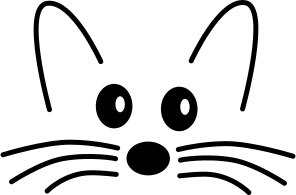
\includegraphics[width=1.4em]{squeak-logo}}}
\newcommand{\dothis}[1]{%
	\medskip
	\noindent\dothisicon
	\ifx#1\empty\else\quad\emph{#1}\fi
	\par\smallskip\nopagebreak}
% NB: To use this in an individual chapter, you must set:
%\graphicspath{{figures/} {../figures/}}
% at the head of the chapter.  Don't forget the final /
%=============================================================
%:Reader hints (hint)
%
% Indicates a non-obvious consequence 
\newcommand{\hint}[1]{\vspace{1ex}\noindent\fbox{\textsc{Astuce}} \emph{#1}}
%=================================================================
% graphics for Morphic handles
\newcommand{\grabHandle}{\raisebox{-0.2ex}{
\includegraphics[width=1em]{blackHandle}}}
\newcommand{\moveHandle}{\raisebox{-0.2ex}{
\includegraphics[width=1em]{moveHandle}}}
\newcommand{\debugHandle}{\raisebox{-0.2ex}{
\includegraphics[width=1em]{debugHandle}}}
% squeak-fr (added for Morphic handles)
\newcommand{\rotateHandle}{\raisebox{-0.2ex}{
\includegraphics[width=1em]{rotateHandle}}}
\newcommand{\viewerHandle}{\raisebox{-0.2ex}{
\includegraphics[width=1em]{viewerHandle}}}
% squeak-fr (add cloverHandle to use \clover in QuickTour.tex as alias
% todo 

%=============================================================
%:Highlighting Important stuff (doublebox)
%
% From Seaside book ...
\newsavebox{\SavedText}
\newlength{\InnerBoxRule}\setlength{\InnerBoxRule}{.75\fboxrule}
\newlength{\OuterBoxRule}\setlength{\OuterBoxRule}{1.5\fboxrule}
\newlength{\BoxSeparation}\setlength{\BoxSeparation}{1.5\fboxrule}
\addtolength{\BoxSeparation}{.5pt}
\newlength{\SaveBoxSep}\setlength{\SaveBoxSep}{2\fboxsep}
%
\newenvironment{doublebox}{\begin{lrbox}{\SavedText}
    \begin{minipage}{.75\textwidth}}
    {\end{minipage}\end{lrbox}\begin{center}
    \setlength{\fboxsep}{\BoxSeparation}\setlength{\fboxrule}{\OuterBoxRule}
    \fbox{\setlength{\fboxsep}{\SaveBoxSep}\setlength{\fboxrule}{\InnerBoxRule}%
      \fbox{\usebox{\SavedText}}}
  \end{center}}
% Use this:
%\newcommand{\important}[1]{\begin{doublebox}#1\end{doublebox}}


\newcommand{\important}[1]{
\noindent\rule{\textwidth}{2pt}\par
\textbf{Important!} #1 \par
\noindent\rule{\textwidth}{2pt}}

\newcommand{\note}[1]{
\noindent\rule{\textwidth}{2pt}\par
\noindent\textbf{Note} #1\par
\noindent\rule{\textwidth}{2pt}}

%=============================================================
%:Section depth
\setcounter{secnumdepth}{2}
%% for this to happen start the file with
%\ifx\wholebook\relax\else
%% $Author$ Martial
% $Date$ Wed Oct 10 13:34:55 CEST 2007
% $Revision$ source: SBE 12715 
% Last Changed Date: 2007-10-08 21:32:45 +0200 (Mon, 08 Oct 2007)
%=============================================================
% NB: documentclass must be set in main document.
% Allows book to be generated in multiple formats.
%=============================================================
%:Packages
%\usepackage[french]{babel}
\usepackage[T1]{fontenc}  %%%%%% really important to get the code directly in the text!
\usepackage{lmodern}
%\usepackage[scaled=0.85]{bookmanx} % needs another scale factor if used with \renewcommand{\sfdefault}{cmbr}
\usepackage{palatino}
%\usepackage[sc]{mathpazo}
%\linespread{1.05}
\usepackage[scaled=0.85]{helvet}
\usepackage{microtype}
\usepackage{graphicx}
\usepackage{theorem}
\usepackage[utf8]{inputenc}
% ON: pdfsync breaks the use of p{width} for tabular columns!
\ifdefined\usepdfsync\usepackage{pdfsync}\fi % Requires texlive 2007
%=============================================================
%:More packages
%Stef should check which ones are used!
%\usepackage{picinpar}
%\usepackage{layout}
%\usepackage{color}
%\definecolor{stefgris}{rgb}{0.85,0.85,0.85}
%\usepackage{enum}
%\usepackage{a4wide}
% \usepackage{fancyhdr}
\usepackage{ifthen}
\usepackage{float}
\usepackage{longtable}
\usepackage{makeidx}
\usepackage[nottoc]{tocbibind}
\usepackage{multicol}
\usepackage{booktabs}	% book-style tables
\usepackage{topcapt}	% enables \topcaption
\usepackage{multirow}
\usepackage{tabularx}
%\usepackage[bottom]{footmisc}
\usepackage{xspace}
\usepackage{alltt}
\usepackage{amssymb,textcomp}
\usepackage[usenames,dvipsnames]{color}
\usepackage{colortbl}
\usepackage[hang]{subfigure}\makeatletter\def\p@subfigure{\thefigure\,}\makeatother
\usepackage{rotating}
\usepackage{enumitem}	% apb: allows more control over tags in enumerations
\usepackage{verbatim}     % for comment environment
\usepackage{varioref}	% for page references that work
\labelformat{footnote}{\thechapter--#1} % to distinguish citations from jurabib
\usepackage{needspace}
\usepackage{isodateo} % enable \isodate
\usepackage[newparttoc]{titlesec}
\usepackage{titletoc}
\usepackage{eurosym}
\usepackage{wrapfig}

\usepackage[
	super,
	citefull=first,
	authorformat={allreversed,and},
	titleformat={commasep,italic}
]{jurabib} % citations as footnotes
\usepackage[
	colorlinks=true,
	linkcolor=black,
	urlcolor=black,
	citecolor=black
]{hyperref}   % should come last

%=============================================================
%:URL style
\makeatletter

\def\url@leostyle{%
  \@ifundefined{selectfont}{\def\UrlFont{\sf}}{\def\UrlFont{\sffamily}}}
% ajouter par Martial pour \traduit (met une dague dans les \doublebox
\def\thempfootnote{\fnsymbol{mpfootnote}}

\makeatother
% Now actually use the newly defined style.
\urlstyle{leo}
%=============================================================
%:Booleans
\newboolean{lulu}
\setboolean{lulu}{false}
\newcommand{\ifluluelse}[2]{\ifthenelse{\boolean{lulu}}{#1}{#2}}
%=============================================================
%:Names
\newcommand{\SUnit}{SUnit\xspace}
\newcommand{\sunit}{SUnit\xspace}
\newcommand{\xUnit}{$x$Unit\xspace}
\newcommand{\JUnit}{JUnit\xspace}
%\newcommand{\XP}{eXtreme Programming\xspace}
\newcommand{\st}{Smalltalk\xspace}
\newcommand{\Squeak}{Squeak\xspace}
\newcommand{\sq}{Squeak\xspace}
\newcommand{\sqmap}{SqueakMap\xspace}
\newcommand{\squeak}{Squeak\xspace}
%\newcommand{\sbe}{\url{scg.unibe.ch/SBE}\xspace}
%\newcommand{\sbe}{\url{squeakbyexample.org}\xspace}
\newcommand{\sbe}{\url{SqueakByExample.org}\xspace}
% squeak-fr: adresse de la version francaise
\newcommand{\spe}{\url{SqueakByExample.org/fr}\xspace}
\newcommand{\sba}{\url{SquareBracketAssociates.org}\xspace}

% squeak-fr: ajout de la \squeakdev pour eviter les problemes de
% changements d'url rencontres dans la VO:
\newcommand{\squeakdev}{\url{www.squeaksource.com/ImageForDevelopers}\xspace} %ou
%\newcommand{\squeakdev}{\url{squeak.ofset.org/squeak-dev}\xspace}

%=============================================================
%:Editorial comment macros
\newcommand{\nnbb}[2]{
    \fbox{\bfseries\sffamily\scriptsize#1}
    {\sf\small$\blacktriangleright$\textit{#2}$\blacktriangleleft$}
   }
\newcommand{\ab}[1]{\nnbb{Andrew}{#1}}
\newcommand{\sd}[1]{\nnbb{St\'{e}f}{#1}}
\newcommand{\md}[1]{\nnbb{Marcus}{#1}}
\newcommand{\on}[1]{\nnbb{Oscar}{#1}}
\newcommand{\damien}[1]{\nnbb{Damien}{#1}}
\newcommand{\lr}[1]{\nnbb{Lukas}{#1}}
\newcommand{\orla}[1]{\nnbb{Orla}{#1}}
%\newcommand{\here}{\nnbb{CONTINUE}{HERE}}
\newcommand{\here}{\nnbb{CONTINUE}{ICI}}

%=============================================================
%:Abbreviation macros
\newcommand{\ie}{\emph{c-\`a-d.}\xspace}
\newcommand{\cad}{\emph{c-\`a-d.}\xspace}
%\newcommand{\eg}{\emph{e.g.},\xspace}
\newcommand{\eg}{\emph{par ex.},\xspace}
\newcommand{\parex}{\emph{par ex.},\xspace}
\newcommand{\etc}{etc\xspace}
%=============================================================
%:Cross reference macros

% [squeak-fr] martial: remarquez les articles devant les noms
\newcommand{\charef}[1]{le chapitre~\ref{cha:#1}\xspace}
% note de martial: utilise dans chapitre Syntax.tex: a redefinir
\newcommand{\charefs}[2]{les chapitres~\ref{cha:#1} et \ref{cha:#2}\xspace}
\newcommand{\secref}[1]{la section~\ref{sec:#1}\xspace}
\newcommand{\figref}[1]{la figure~\ref{fig:#1}\xspace}
\newcommand{\Figref}[1]{La figure~\ref{fig:#1}\xspace}
\newcommand{\appref}[1]{l'annexe~\ref{app:#1}\xspace}
\newcommand{\tabref}[1]{la table~\ref{tab:#1}\xspace}
% defini pour le chapitre Messages.tex
\newcommand{\Tabref}[1]{La table~\ref{tab:#1}\xspace}

% APB: I removed trailing \xspace commands from these macros because
% \xspace mostly doesn't work.  If you want a space after your
% references, type one!
% ON: xspace has always worked just fine for me!  Please leave them in.
%
\newcommand{\ruleref}[1]{\ref{rule:#1}\xspace}
%
\newcommand{\egref}[1]{exemple~\ref{eg:#1}\xspace}
\newcommand{\Egref}[1]{Exemple~\ref{eg:#1}\xspace}
%
\newcommand{\scrref}[1]{script~\ref{scr:#1}\xspace}
\newcommand{\Scrref}[1]{Script~\ref{scr:#1}\xspace}
% t = the
\newcommand{\tscrref}[1]{le script~\ref{scr:#1}\xspace}
\newcommand{\Tscrref}[1]{Le script~\ref{scr:#1}\xspace}
%
\newcommand{\mthref}[1]{m\'ethode~\ref{mth:#1}\xspace}
\newcommand{\mthsref}[1]{m\'ethodes~\ref{mth:#1}\xspace}
\newcommand{\Mthref}[1]{M\'ethode~\ref{mth:#1}\xspace}
\newcommand{\tmthref}[1]{la m\'ethode~\ref{mth:#1}\xspace}
\newcommand{\Tmthref}[1]{La m\'ethode~\ref{mth:#1}\xspace}
%
\newcommand{\clsref}[1]{classe~\ref{cls:#1}\xspace}
\newcommand{\tclsref}[1]{la classe~\ref{cls:#1}\xspace}
\newcommand{\Tclsref}[1]{La classe~\ref{cls:#1}\xspace}
%=============================================================
%:Menu item macro
% for menu items, so we can change our minds on how to print them! (apb)
\definecolor{lightgray}{gray}{0.89}
\newcommand{\menu}[1]{{%
	\setlength{\fboxsep}{0pt}%
	\colorbox{lightgray}{{{\upshape\sffamily\strut \,#1\,}}}}}
% \newcommand{\menu}[1]{{%
% 	\fontfamily{lmr}\selectfont
% 	\upshape\textlangle{\sffamily #1}\textrangle}}
% For submenu items:
\newcommand{\go}{\,$\triangleright$\,}
% \newcommand{\go}{\,$\blacktriangleright$\,}
% For keyboard shortcuts:
%\newcommand{\short}[1]{\mbox{$\langle${\sc CMD}$\rangle$-#1}\xspace}
\newcommand{\short}[1]{\mbox{{\sc cmd}\hspace{0.08em}--\hspace{0.09em}#1}\xspace}
% For buttons:
\newcommand{\button}[1]{{%
	\setlength{\fboxsep}{0pt}%
	\fbox{{\upshape\sffamily\strut \,#1\,}}}}
\newcommand{\toolsflap}{l'onglet \textit{Tools}\xspace}
%=============================================================
%:Reader cues (do this)
%
% Indicate something the reader should try out.
\newcommand{\dothisicon}{\raisebox{-.5ex}{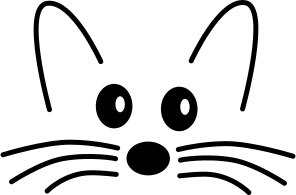
\includegraphics[width=1.4em]{squeak-logo}}}
\newcommand{\dothis}[1]{%
	\medskip
	\noindent\dothisicon
	\ifx#1\empty\else\quad\emph{#1}\fi
	\par\smallskip\nopagebreak}
% NB: To use this in an individual chapter, you must set:
%\graphicspath{{figures/} {../figures/}}
% at the head of the chapter.  Don't forget the final /
%=============================================================
%:Reader hints (hint)
%
% Indicates a non-obvious consequence 
\newcommand{\hint}[1]{\vspace{1ex}\noindent\fbox{\textsc{Astuce}} \emph{#1}}
%=================================================================
% graphics for Morphic handles
\newcommand{\grabHandle}{\raisebox{-0.2ex}{
\includegraphics[width=1em]{blackHandle}}}
\newcommand{\moveHandle}{\raisebox{-0.2ex}{
\includegraphics[width=1em]{moveHandle}}}
\newcommand{\debugHandle}{\raisebox{-0.2ex}{
\includegraphics[width=1em]{debugHandle}}}
% squeak-fr (added for Morphic handles)
\newcommand{\rotateHandle}{\raisebox{-0.2ex}{
\includegraphics[width=1em]{rotateHandle}}}
\newcommand{\viewerHandle}{\raisebox{-0.2ex}{
\includegraphics[width=1em]{viewerHandle}}}
% squeak-fr (add cloverHandle to use \clover in QuickTour.tex as alias
% todo 

%=============================================================
%:Highlighting Important stuff (doublebox)
%
% From Seaside book ...
\newsavebox{\SavedText}
\newlength{\InnerBoxRule}\setlength{\InnerBoxRule}{.75\fboxrule}
\newlength{\OuterBoxRule}\setlength{\OuterBoxRule}{1.5\fboxrule}
\newlength{\BoxSeparation}\setlength{\BoxSeparation}{1.5\fboxrule}
\addtolength{\BoxSeparation}{.5pt}
\newlength{\SaveBoxSep}\setlength{\SaveBoxSep}{2\fboxsep}
%
\newenvironment{doublebox}{\begin{lrbox}{\SavedText}
    \begin{minipage}{.75\textwidth}}
    {\end{minipage}\end{lrbox}\begin{center}
    \setlength{\fboxsep}{\BoxSeparation}\setlength{\fboxrule}{\OuterBoxRule}
    \fbox{\setlength{\fboxsep}{\SaveBoxSep}\setlength{\fboxrule}{\InnerBoxRule}%
      \fbox{\usebox{\SavedText}}}
  \end{center}}
% Use this:
%\newcommand{\important}[1]{\begin{doublebox}#1\end{doublebox}}


\newcommand{\important}[1]{
\noindent\rule{\textwidth}{2pt}\par
\textbf{Important!} #1 \par
\noindent\rule{\textwidth}{2pt}}

\newcommand{\note}[1]{
\noindent\rule{\textwidth}{2pt}\par
\noindent\textbf{Note} #1\par
\noindent\rule{\textwidth}{2pt}}

%=============================================================
%:Section depth
\setcounter{secnumdepth}{2}
%% for this to happen start the file with
%\ifx\wholebook\relax\else
%% $Author$ Martial
% $Date$ Wed Oct 10 13:34:55 CEST 2007
% $Revision$ source: SBE 12715 
% Last Changed Date: 2007-10-08 21:32:45 +0200 (Mon, 08 Oct 2007)
%=============================================================
% NB: documentclass must be set in main document.
% Allows book to be generated in multiple formats.
%=============================================================
%:Packages
%\usepackage[french]{babel}
\usepackage[T1]{fontenc}  %%%%%% really important to get the code directly in the text!
\usepackage{lmodern}
%\usepackage[scaled=0.85]{bookmanx} % needs another scale factor if used with \renewcommand{\sfdefault}{cmbr}
\usepackage{palatino}
%\usepackage[sc]{mathpazo}
%\linespread{1.05}
\usepackage[scaled=0.85]{helvet}
\usepackage{microtype}
\usepackage{graphicx}
\usepackage{theorem}
\usepackage[utf8]{inputenc}
% ON: pdfsync breaks the use of p{width} for tabular columns!
\ifdefined\usepdfsync\usepackage{pdfsync}\fi % Requires texlive 2007
%=============================================================
%:More packages
%Stef should check which ones are used!
%\usepackage{picinpar}
%\usepackage{layout}
%\usepackage{color}
%\definecolor{stefgris}{rgb}{0.85,0.85,0.85}
%\usepackage{enum}
%\usepackage{a4wide}
% \usepackage{fancyhdr}
\usepackage{ifthen}
\usepackage{float}
\usepackage{longtable}
\usepackage{makeidx}
\usepackage[nottoc]{tocbibind}
\usepackage{multicol}
\usepackage{booktabs}	% book-style tables
\usepackage{topcapt}	% enables \topcaption
\usepackage{multirow}
\usepackage{tabularx}
%\usepackage[bottom]{footmisc}
\usepackage{xspace}
\usepackage{alltt}
\usepackage{amssymb,textcomp}
\usepackage[usenames,dvipsnames]{color}
\usepackage{colortbl}
\usepackage[hang]{subfigure}\makeatletter\def\p@subfigure{\thefigure\,}\makeatother
\usepackage{rotating}
\usepackage{enumitem}	% apb: allows more control over tags in enumerations
\usepackage{verbatim}     % for comment environment
\usepackage{varioref}	% for page references that work
\labelformat{footnote}{\thechapter--#1} % to distinguish citations from jurabib
\usepackage{needspace}
\usepackage{isodateo} % enable \isodate
\usepackage[newparttoc]{titlesec}
\usepackage{titletoc}
\usepackage{eurosym}
\usepackage{wrapfig}

\usepackage[
	super,
	citefull=first,
	authorformat={allreversed,and},
	titleformat={commasep,italic}
]{jurabib} % citations as footnotes
\usepackage[
	colorlinks=true,
	linkcolor=black,
	urlcolor=black,
	citecolor=black
]{hyperref}   % should come last

%=============================================================
%:URL style
\makeatletter

\def\url@leostyle{%
  \@ifundefined{selectfont}{\def\UrlFont{\sf}}{\def\UrlFont{\sffamily}}}
% ajouter par Martial pour \traduit (met une dague dans les \doublebox
\def\thempfootnote{\fnsymbol{mpfootnote}}

\makeatother
% Now actually use the newly defined style.
\urlstyle{leo}
%=============================================================
%:Booleans
\newboolean{lulu}
\setboolean{lulu}{false}
\newcommand{\ifluluelse}[2]{\ifthenelse{\boolean{lulu}}{#1}{#2}}
%=============================================================
%:Names
\newcommand{\SUnit}{SUnit\xspace}
\newcommand{\sunit}{SUnit\xspace}
\newcommand{\xUnit}{$x$Unit\xspace}
\newcommand{\JUnit}{JUnit\xspace}
%\newcommand{\XP}{eXtreme Programming\xspace}
\newcommand{\st}{Smalltalk\xspace}
\newcommand{\Squeak}{Squeak\xspace}
\newcommand{\sq}{Squeak\xspace}
\newcommand{\sqmap}{SqueakMap\xspace}
\newcommand{\squeak}{Squeak\xspace}
%\newcommand{\sbe}{\url{scg.unibe.ch/SBE}\xspace}
%\newcommand{\sbe}{\url{squeakbyexample.org}\xspace}
\newcommand{\sbe}{\url{SqueakByExample.org}\xspace}
% squeak-fr: adresse de la version francaise
\newcommand{\spe}{\url{SqueakByExample.org/fr}\xspace}
\newcommand{\sba}{\url{SquareBracketAssociates.org}\xspace}

% squeak-fr: ajout de la \squeakdev pour eviter les problemes de
% changements d'url rencontres dans la VO:
\newcommand{\squeakdev}{\url{www.squeaksource.com/ImageForDevelopers}\xspace} %ou
%\newcommand{\squeakdev}{\url{squeak.ofset.org/squeak-dev}\xspace}

%=============================================================
%:Editorial comment macros
\newcommand{\nnbb}[2]{
    \fbox{\bfseries\sffamily\scriptsize#1}
    {\sf\small$\blacktriangleright$\textit{#2}$\blacktriangleleft$}
   }
\newcommand{\ab}[1]{\nnbb{Andrew}{#1}}
\newcommand{\sd}[1]{\nnbb{St\'{e}f}{#1}}
\newcommand{\md}[1]{\nnbb{Marcus}{#1}}
\newcommand{\on}[1]{\nnbb{Oscar}{#1}}
\newcommand{\damien}[1]{\nnbb{Damien}{#1}}
\newcommand{\lr}[1]{\nnbb{Lukas}{#1}}
\newcommand{\orla}[1]{\nnbb{Orla}{#1}}
%\newcommand{\here}{\nnbb{CONTINUE}{HERE}}
\newcommand{\here}{\nnbb{CONTINUE}{ICI}}

%=============================================================
%:Abbreviation macros
\newcommand{\ie}{\emph{c-\`a-d.}\xspace}
\newcommand{\cad}{\emph{c-\`a-d.}\xspace}
%\newcommand{\eg}{\emph{e.g.},\xspace}
\newcommand{\eg}{\emph{par ex.},\xspace}
\newcommand{\parex}{\emph{par ex.},\xspace}
\newcommand{\etc}{etc\xspace}
%=============================================================
%:Cross reference macros

% [squeak-fr] martial: remarquez les articles devant les noms
\newcommand{\charef}[1]{le chapitre~\ref{cha:#1}\xspace}
% note de martial: utilise dans chapitre Syntax.tex: a redefinir
\newcommand{\charefs}[2]{les chapitres~\ref{cha:#1} et \ref{cha:#2}\xspace}
\newcommand{\secref}[1]{la section~\ref{sec:#1}\xspace}
\newcommand{\figref}[1]{la figure~\ref{fig:#1}\xspace}
\newcommand{\Figref}[1]{La figure~\ref{fig:#1}\xspace}
\newcommand{\appref}[1]{l'annexe~\ref{app:#1}\xspace}
\newcommand{\tabref}[1]{la table~\ref{tab:#1}\xspace}
% defini pour le chapitre Messages.tex
\newcommand{\Tabref}[1]{La table~\ref{tab:#1}\xspace}

% APB: I removed trailing \xspace commands from these macros because
% \xspace mostly doesn't work.  If you want a space after your
% references, type one!
% ON: xspace has always worked just fine for me!  Please leave them in.
%
\newcommand{\ruleref}[1]{\ref{rule:#1}\xspace}
%
\newcommand{\egref}[1]{exemple~\ref{eg:#1}\xspace}
\newcommand{\Egref}[1]{Exemple~\ref{eg:#1}\xspace}
%
\newcommand{\scrref}[1]{script~\ref{scr:#1}\xspace}
\newcommand{\Scrref}[1]{Script~\ref{scr:#1}\xspace}
% t = the
\newcommand{\tscrref}[1]{le script~\ref{scr:#1}\xspace}
\newcommand{\Tscrref}[1]{Le script~\ref{scr:#1}\xspace}
%
\newcommand{\mthref}[1]{m\'ethode~\ref{mth:#1}\xspace}
\newcommand{\mthsref}[1]{m\'ethodes~\ref{mth:#1}\xspace}
\newcommand{\Mthref}[1]{M\'ethode~\ref{mth:#1}\xspace}
\newcommand{\tmthref}[1]{la m\'ethode~\ref{mth:#1}\xspace}
\newcommand{\Tmthref}[1]{La m\'ethode~\ref{mth:#1}\xspace}
%
\newcommand{\clsref}[1]{classe~\ref{cls:#1}\xspace}
\newcommand{\tclsref}[1]{la classe~\ref{cls:#1}\xspace}
\newcommand{\Tclsref}[1]{La classe~\ref{cls:#1}\xspace}
%=============================================================
%:Menu item macro
% for menu items, so we can change our minds on how to print them! (apb)
\definecolor{lightgray}{gray}{0.89}
\newcommand{\menu}[1]{{%
	\setlength{\fboxsep}{0pt}%
	\colorbox{lightgray}{{{\upshape\sffamily\strut \,#1\,}}}}}
% \newcommand{\menu}[1]{{%
% 	\fontfamily{lmr}\selectfont
% 	\upshape\textlangle{\sffamily #1}\textrangle}}
% For submenu items:
\newcommand{\go}{\,$\triangleright$\,}
% \newcommand{\go}{\,$\blacktriangleright$\,}
% For keyboard shortcuts:
%\newcommand{\short}[1]{\mbox{$\langle${\sc CMD}$\rangle$-#1}\xspace}
\newcommand{\short}[1]{\mbox{{\sc cmd}\hspace{0.08em}--\hspace{0.09em}#1}\xspace}
% For buttons:
\newcommand{\button}[1]{{%
	\setlength{\fboxsep}{0pt}%
	\fbox{{\upshape\sffamily\strut \,#1\,}}}}
\newcommand{\toolsflap}{l'onglet \textit{Tools}\xspace}
%=============================================================
%:Reader cues (do this)
%
% Indicate something the reader should try out.
\newcommand{\dothisicon}{\raisebox{-.5ex}{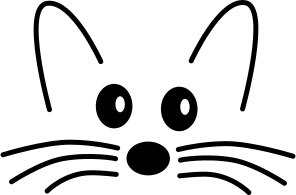
\includegraphics[width=1.4em]{squeak-logo}}}
\newcommand{\dothis}[1]{%
	\medskip
	\noindent\dothisicon
	\ifx#1\empty\else\quad\emph{#1}\fi
	\par\smallskip\nopagebreak}
% NB: To use this in an individual chapter, you must set:
%\graphicspath{{figures/} {../figures/}}
% at the head of the chapter.  Don't forget the final /
%=============================================================
%:Reader hints (hint)
%
% Indicates a non-obvious consequence 
\newcommand{\hint}[1]{\vspace{1ex}\noindent\fbox{\textsc{Astuce}} \emph{#1}}
%=================================================================
% graphics for Morphic handles
\newcommand{\grabHandle}{\raisebox{-0.2ex}{
\includegraphics[width=1em]{blackHandle}}}
\newcommand{\moveHandle}{\raisebox{-0.2ex}{\includegraphics[width=1em]{moveHandle}}}
\newcommand{\debugHandle}{\raisebox{-0.2ex}{\includegraphics[width=1em]{debugHandle}}}
% squeak-fr (added for Morphic handles)
\newcommand{\rotateHandle}{\raisebox{-0.2ex}{\includegraphics[width=1em]{rotateHandle}}}
\newcommand{\viewerHandle}{\raisebox{-0.2ex}{\includegraphics[width=1em]{viewerHandle}}}
% squeak-fr (add cloverHandle to use \clover in QuickTour.tex as alias
% todo 

%=============================================================
%:Highlighting Important stuff (doublebox)
%
% From Seaside book ...
\newsavebox{\SavedText}
\newlength{\InnerBoxRule}\setlength{\InnerBoxRule}{.75\fboxrule}
\newlength{\OuterBoxRule}\setlength{\OuterBoxRule}{1.5\fboxrule}
\newlength{\BoxSeparation}\setlength{\BoxSeparation}{1.5\fboxrule}
\addtolength{\BoxSeparation}{.5pt}
\newlength{\SaveBoxSep}\setlength{\SaveBoxSep}{2\fboxsep}
%
\newenvironment{doublebox}{\begin{lrbox}{\SavedText}
    \begin{minipage}{.75\textwidth}}
    {\end{minipage}\end{lrbox}\begin{center}
    \setlength{\fboxsep}{\BoxSeparation}\setlength{\fboxrule}{\OuterBoxRule}
    \fbox{\setlength{\fboxsep}{\SaveBoxSep}\setlength{\fboxrule}{\InnerBoxRule}%
      \fbox{\usebox{\SavedText}}}
  \end{center}}
% Use this:
%\newcommand{\important}[1]{\begin{doublebox}#1\end{doublebox}}


\newcommand{\important}[1]{
\noindent\rule{\textwidth}{2pt}\par
\textbf{Important!} #1 \par
\noindent\rule{\textwidth}{2pt}}

\newcommand{\note}[1]{
\noindent\rule{\textwidth}{2pt}\par
\noindent\textbf{Note} #1\par
\noindent\rule{\textwidth}{2pt}}

%=============================================================
%:Section depth
\setcounter{secnumdepth}{2}
%% for this to happen start the file with
%\ifx\wholebook\relax\else
%\input{../common.tex}
%\begin{document}
%\fi
% and terminate by
% \ifx\wholebook\relax\else\end{document}\fi

\DeclareGraphicsExtensions{.pdf, .jpg, .png}
%=============================================================
%:PDF setup
\hypersetup{
%   a4paper,
%   pdfstartview=FitV,
%   colorlinks,
%   linkcolor=darkblue,
%   citecolor=darkblue,
%   pdftitle={Squeak by Example},
pdftitle={Squeak par l'exemple},
   pdfauthor={Andrew Black, St\'ephane Ducasse,	Oscar Nierstrasz,
Damien Pollet},
   pdfkeywords={Smalltalk, Squeak, Programmation Orient\'ee Objet},
pdfsubject={Informatique, Computer Science}
}
%=============================================================
%:Page layout and appearance
%
% \renewcommand{\headrulewidth}{0pt}
\renewcommand{\chaptermark}[1]{\markboth{#1}{}}
\renewcommand{\sectionmark}[1]{\markright{\thesection\ #1}}
\renewpagestyle{plain}[\small\itshape]{%
	\setheadrule{0pt}%
	\sethead[][][]{}{}{}%
	\setfoot[][][]{}{}{}}
\renewpagestyle{headings}[\small\itshape]{%
	\setheadrule{0pt}%
	\setmarks{chapter}{section}%
	\sethead[\thepage][][\chaptertitle]{\sectiontitle}{}{\thepage}%
	\setfoot[][][]{}{}{}}
% pagestyle for tableofcontents + index (martial: 2008/04/23)
\newpagestyle{newheadings}[\small\itshape]{%
	\setheadrule{0pt}%
	\setmarks{chapter}{section}%
	\sethead[\thepage][][\chaptertitle]{\chaptertitle}{}{\thepage}%
	\setfoot[][][]{}{}{}}
%=============================================================
%:Title section setup and TOC numbering depth
\setcounter{secnumdepth}{1}
\setcounter{tocdepth}{1}
\titleformat{\part}[display]{\centering}{\huge\partname\ \thepart}{1em}{\Huge\textbf}[]
\titleformat{\chapter}[display]{}{\huge\chaptertitlename\ \thechapter}{1em}{\Huge\raggedright\textbf}[]
\titlecontents{part}[3pc]{%
		\pagebreak[2]\addvspace{1em plus.4em minus.2em}%
		\leavevmode\large\bfseries}
	{\contentslabel{3pc}}{\hspace*{-3pc}}
	{}[\nopagebreak]
\titlecontents{chapter}[3pc]{%
		\pagebreak[0]\addvspace{1em plus.2em minus.2em}%
		\leavevmode\bfseries}
	{\contentslabel{3pc}}{}
	{\hfill\contentspage}[\nopagebreak]
\dottedcontents{section}[3pc]{}{3pc}{1pc}
\dottedcontents{subsection}[3pc]{}{0pc}{1pc}
% \dottedcontents{subsection}[4.5em]{}{0pt}{1pc}
% Make \cleardoublepage insert really blank pages http://www.tex.ac.uk/cgi-bin/texfaq2html?label=reallyblank
\let\origdoublepage\cleardoublepage
\newcommand{\clearemptydoublepage}{%
  \clearpage
  {\pagestyle{empty}\origdoublepage}}
\let\cleardoublepage\clearemptydoublepage % see http://www.tex.ac.uk/cgi-bin/texfaq2html?label=patch
%=============================================================
%:FAQ macros (for FAQ chapter)
\newtheorem{faq}{FAQ}
\newcommand{\answer}{\paragraph{R\'eponse}\ }
%=============================================================
%:Listings package configuration
\usepackage{listings}
\newcommand{\caret}{\makebox{\raisebox{0.4ex}{\footnotesize{$\wedge$}}}}
\lstdefinelanguage{Smalltalk}{
%  morekeywords={self,super,true,false,nil,thisContext}, % This is overkill
  morestring=[d]',
  morecomment=[s]{"}{"},
  alsoletter={\#:},
  escapechar={!},
  escapebegin=\itshape, % comment-like by default (Martial 11/2007)
  literate=
    {BANG}{!}1
    {UNDERSCORE}{\_}1
    {\\st}{Smalltalk}9 % convenience -- in case \st occurs in code
    % {'}{{\textquotesingle}}1 % replaced by upquote=true in \lstset
    {_}{{$\leftarrow$}}1
    {>>>}{{\sep}}1
    {^}{{$\uparrow$}}1
    {~}{{$\sim$}}1
    {-}{{\sf -\hspace{-0.13em}-}}1  % the goal is to make - the same width as +
    {+}{\raisebox{0.08ex}{+}}1		% and to raise + off the baseline to match -
    {-->}{{\quad$\longrightarrow$\quad}}3
	, % Don't forget the comma at the end!
  tabsize=4
}[keywords,comments,strings]
% ajout pour les échappements dans les codes
% indispensable pour mettre le code en emphase (cf. Model.tex) 
\newcommand{\codeify}[1]{\NoAutoSpaceBeforeFDP#1\AutoSpaceBeforeFDP}
\newcommand{\normcomment}[1]{\emph{#1}} %cf. Streams
\newcommand{\normcode}[1]{\emph{\codeify{#1}}} %cf. Streams
\newcommand{\emcode}[1]{\textbf{\normcode{#1}}} % Martial 11/2007
\lstset{language=Smalltalk,
	basicstyle=\sffamily,
	keywordstyle=\color{black}\bfseries,
	% stringstyle=\ttfamily, % Ugly! do we really want this? -- on
	%commentstyle=\itshape,
	mathescape=true,
	showstringspaces=false,
	keepspaces=true,
	breaklines=true,
	breakautoindent=true,
	lineskip={-1pt}, % Ugly hack
	upquote=true, % straight quote; requires textcomp package
	columns=fullflexible} % no fixed width fonts
% In-line code (literal)
% Normally use this for all in-line code:
\newcommand{\ct}{\lstinline[mathescape=false,basicstyle={\sffamily\upshape}]}
% apb 2007.8.28 added the \upshape declaration to avoid getting italicized code in \dothis{ } sections.
% In-line code (latex enabled)
% Use this only in special situations where \ct does not work
% (within section headings ...):

% [squeak-fr] Modification de \lct suivant les indications de Martial Boniou
\newcommand{\lct}[1]{\textsf{\textup{\NoAutoSpaceBeforeFDP #1
\AutoSpaceBeforeFDP}}} %\xspace

% Use these for system categories and protocols:
\newcommand{\scat}[1]{\emph{\textsf{#1}}\xspace}
\newcommand{\pkg}[1]{\emph{\textsf{#1}}\xspace}
\newcommand{\prot}[1]{\emph{\textsf{#1}}\xspace}
% Code environments
% NB: the arg is for tests
% Only code and example environments may be tests
\lstnewenvironment{code}[1]{%
	\lstset{%
		frame=lines,
		mathescape=false
	}
}{}
\def\ignoredollar#1{}
%=============================================================
%:Code environments (method, script ...)
% NB: the third arg is for tests
% Only code and example environments may be tests
\lstnewenvironment{example}[3][defaultlabel]{%
	\renewcommand{\lstlistingname}{Exemple}%
	\lstset{
		frame=lines,
		mathescape=false,
		caption={\emph{#2}},
		label={eg:#1}
	}
}{}
\lstnewenvironment{script}[2][defaultlabel]{%
\renewcommand{\lstlistingname}{Script}%
	\lstset{
		frame=lines,
		mathescape=false,
		name={Script},
		caption={\emph{#2}},
		label={scr:#1}
	}
}{}
%I could not find a way yo get the Experiment #numb followed by the caption in a black box
%\colorbox{black}{\makebox[\textwidth]{  \color{white} {\large {\bfseries Experiment 3-1 (crear i moure un robot)}} }}
\lstnewenvironment{experiment}[2][defaultlabel]{%
%\noindent\rule{\textwidth}{2pt}\vspace{-0.8cm}
\renewcommand{\lstlistingname}{Experiment}%
	\lstset{
		frame=none,
		rulecolor=\color{black},
		mathescape=false,
		name={Experiment},
		caption={\emph{#2}},
		label={scr:#1}
	}
}{%\vspace{-0.5cm}\noindent\rule{\textwidth}{2pt}
}

\lstnewenvironment{method}[2][defaultlabel]{%
	\renewcommand{\lstlistingname}{Method}%
	\lstset{
		frame=lines,
		mathescape=false,
		name={M\'ethode},
		caption={\emph{#2}},
		label={mth:#1}
	}
}{}
\lstnewenvironment{methods}[2][defaultlabel]{% just for multiple methods at once
	\renewcommand{\lstlistingname}{Methods}%
	\lstset{
		frame=lines,
		mathescape=false,
		name={M\'ethode},
		caption={\emph{#2}},
		label={mth:#1}
	}
}{}
\lstnewenvironment{numMethod}[2][defaultlabel]{%
	\renewcommand{\lstlistingname}{Method}%
	\lstset{
		numbers=left,
		numberstyle={\tiny\sffamily},
		frame=lines,
		mathescape=false,
		name={M\'ethode},
		caption={\emph{#2}},
		label={mth:#1}
	}
}{}
% \lstnewenvironment{classdef}[2][defaultlabel]{%
% 	\renewcommand{\lstlistingname}{Classe}%
% 	\lstset{
% 		frame=lines,
% 		mathescape=false,
% 		name={Classe},
% 		caption={\emph{#2}},
% 		label={cls:#1}
% 	}
% }{}

%%%%%%%%%%%%%%%%%%%%%%%%%%%%%%%%%%%%%%%%%%%%%%%%%%%%%%%%%%%%%%%%%%%%%%%%%%%%%%%%%%%%%%%%%%%%%%%%%
%%From the original book latex template
%%%%%%%%%%%%%%%%%%%%%%%%%%%%%%%%%%%%%%%%%%%%%%%%%%%%%%%%%%%%%%%%%%%%%%%%%%%%%%%%%%%%%%%%%%%%%%%%%
\theoremstyle{break}
{\theorembodyfont{\rmfamily}\theoremstyle{break}
\newtheorem{privScript}{Script}[chapter]
%\newtheorem{privMethod}{Method}[chapter]
\newtheorem{privExercise}{Experiment}[chapter]}

% \theoremstyle{break}
% {\theorembodyfont{\rmfamily} \newtheorem{privMethod}{Method}[chapter]}

%class
\theoremstyle{break}
{\theorembodyfont{\rmfamily} \newtheorem{privClassDef}{Class}[chapter]}

%important
\theoremstyle{break}
{\theorembodyfont{\rmfamily} \newtheorem{privTemplate}{Important Messages}[chapter]}

% experiment
\newenvironment{exercise}
    {\begin{privExercise}\mbox{}\\}
    {\end{privExercise}}


%%% for figure
\newsavebox{\ScriptFigure}
\newlength{\ScriptWidth}
\newlength{\FigureWidth}

%%%%%%%%%%%%%%%%%%%%%%%%%%%%%%%%%%%%%%%%%%%%%%%%%%%%%%%%%%%%%%%%%%%%%%%%%%%%%%%%
\newenvironment{scriptfig}[3][0.6]
   {\setlength{\ScriptWidth}{\linewidth*\real{#1}}%
   \setlength{\FigureWidth}{\linewidth-(\linewidth*\real{#1})}%
   \savebox{\ScriptFigure}%
	{\parbox{\FigureWidth}{\includegraphics[width=0.98\FigureWidth]{#2}}}%
   \par\noindent\begin{minipage}{\linewidth}\hrule\vskip 0.2cm\begin{minipage}[c]{\ScriptWidth}%
   \begin{stefscript}[{\em #3}]\begin{alltt}\sffamily}
   {\end{alltt}\end{stefscript}\end{minipage}\hfill
   \usebox{\ScriptFigure}
   \vskip 1ex\hrule\end{minipage}\vskip 1ex\par}

%%%%%%%%%%%%%%%%%%%%%%%%%%%%%%%%%%%%%%%%%%%%%%%%%%%%%%%%%%%%%%%%%%%%%%%%%%%%%%%%
%% to be able to specify the complete set of values for includegraphics
%% may be will be changed but not the interface
\newenvironment{scriptfigwithsize}[3][0.6]
   {\setlength{\ScriptWidth}{\linewidth*\real{#1}}%
   \setlength{\FigureWidth}{\linewidth-(\linewidth*\real{#1})}%
   \savebox{\ScriptFigure}{\parbox{\FigureWidth}{\raggedleft{#2}}}%
   \par\noindent\begin{minipage}{\linewidth}\hrule\vskip 0.3cm\begin{minipage}[c]{\ScriptWidth}%
   \begin{stefscript}[{\em #3}]\begin{alltt}\sffamily}
   {\end{alltt}\end{stefscript}\end{minipage}\hfill
   \usebox{\ScriptFigure}
   \vskip 1ex\hrule\end{minipage}\vskip 1ex\par}

% \newenvironment{methodfig}[2][0.6]
%    {\setlength{\ScriptWidth}{\linewidth*\real{#1}}%
%    \setlength{\FigureWidth}{\linewidth-(\linewidth*\real{#1})}%
%    \savebox{\ScriptFigure}{\parbox{\FigureWidth}{\includegraphics[width=.98\FigureWidth]{#2}}}%
%    \par\noindent\rule{\linewidth}{1mm}
%    \\[-0.3cm]\noindent\rule{\linewidth}{0.1mm}
%    \noindent\begin{minipage}[c]{\ScriptWidth}\begin{privMethod}\begin{alltt}\sffamily}
%    {\end{alltt}\end{privMethod}\end{minipage}\hfill
%    \usebox{\ScriptFigure} \vskip 1ex\hrule\vskip 1ex\par}

% \newenvironment{method}
% {\par\noindent\begin{minipage}{\linewidth}\vspace{0.2cm}\begin{privMethod}\begin{nminipage}\vspace{-0.2cm}\rule{\linewidth}{1mm}\\[-0.6cm]\rule{\linewidth}{0.1mm}\end{nminipage}\hspace*{\scriptindent}\codesize\begin{nalltt}\vspace{-0.2cm}}
% {\end{nalltt}\normalsize\vspace{-0.1cm}\hrule\end{privMethod}\vspace{0.2cm}\end{minipage}}


% \newenvironment{classdef}
% {\par\noindent\begin{minipage}{\linewidth}\vspace{0.2cm}\begin{privClassDef}\begin{nminipage}\vspace{-0.2cm}\rule{\linewidth}{1mm}\\[-0.6cm]\rule{\linewidth}{0.1mm}\end{nminipage}\hspace*{\scriptindent}\codesize\begin{nalltt}\vspace{-0.2cm}}
% {\end{nalltt}\normalsize\vspace{-0.1cm}\hrule\end{privClassDef}\vspace{0.2cm}\end{minipage}}


% \newenvironment{template}
% {\par\noindent\begin{minipage}{\linewidth}\vspace{0.3cm}\begin{privTemplate}\begin{nminipage}\vspace{-0.4cm}\rule{\linewidth}{0.1mm}\end{nminipage}\hspace*{\scriptindent}\begin{nalltt}\vspace{-0.7cm}}
% {\end{nalltt}\vspace{-0.1cm}\hrule\end{privTemplate}\end{minipage}\vspace{0.3cm}}

\newenvironment{exofig}[2][0.7]
   {\setlength{\ScriptWidth}{\linewidth*\real{#1}}
   \setlength{\FigureWidth}{\linewidth-(\linewidth*\real{#1})}
   \savebox{\ScriptFigure}{\parbox{\FigureWidth}{\raggedleft{\includegraphics[width=.98\FigureWidth]{#2}}}}
   \par\noindent\begin{minipage}{\linewidth}\hrule\vskip 0.3cm\begin{minipage}[c]{\ScriptWidth}%
   \begin{privExercise}}
   {\end{privExercise}\end{minipage}\hfill
   \usebox{\ScriptFigure}
   \vskip 1ex\hrule\end{minipage}\vskip 1ex\par}

\newenvironment{exofigwithsize}[2][0.7]
   {\setlength{\ScriptWidth}{\linewidth*\real{#1}}
   \setlength{\FigureWidth}{\linewidth-(\linewidth*\real{#1})}
   \savebox{\ScriptFigure}{\parbox{\FigureWidth}{\raggedleft{#2}}}
   \par\noindent\begin{minipage}{\linewidth}\hrule\vskip 0.3cm\begin{minipage}[c]{\ScriptWidth}%
   \begin{privExercise}}
   {\end{privExercise}\end{minipage}\hfill\usebox{\ScriptFigure}
   \vskip 1ex\hrule\end{minipage}\vskip 1ex\par}

\newenvironment{exofigwithsizeandtitle}[3][0.7]
   {\setlength{\ScriptWidth}{\linewidth*\real{#1}}
   \setlength{\FigureWidth}{\linewidth-(\linewidth*\real{#1})}
   \savebox{\ScriptFigure}{\parbox{\FigureWidth}{\raggedleft{#2}}}
   \vskip 0.3cm\par\noindent\begin{minipage}{\linewidth}\hrule\vskip 0.1cm\begin{minipage}[c]{\ScriptWidth}%
   \begin{privExercise}[\em{#3}]}
   {\end{privExercise}\end{minipage}\hfill\usebox{\ScriptFigure}
   \vskip 1ex\hrule\end{minipage}\vskip 1ex\par}

\newenvironment{exofigwithtitle}[3][0.7]
   {\setlength{\ScriptWidth}{\linewidth*\real{#1}}
   \setlength{\FigureWidth}{\linewidth-(\linewidth*\real{#1})}
   \savebox{\ScriptFigure}{\parbox{\FigureWidth}{\raggedleft{\includegraphics[width=.98\FigureWidth]{#2}}}}
   \par\noindent\begin{minipage}{\linewidth}\hrule\vskip 0.3cm\begin{minipage}[c]{\ScriptWidth}%
   \begin{privExercise}[\em{#3}]}
   {\end{privExercise}\end{minipage}\hfill
   \usebox{\ScriptFigure}
   \vskip 1ex\hrule\end{minipage}\vskip 1ex\par}


\newenvironment{exonofigwithtitle}[3][0.7]
   {\setlength{\ScriptWidth}{\linewidth*\real{#1}}
   \setlength{\FigureWidth}{\linewidth-(\linewidth*\real{#1})}
   \savebox{\ScriptFigure}{\parbox{\FigureWidth}{\raggedleft{\includegraphics[width=.98\FigureWidth]{#2}}}}
   \par\noindent\begin{minipage}{\linewidth}\hrule\vskip 0.3cm\begin{minipage}[c]{\ScriptWidth}%
   \begin{privExercise}[\em{#3}]}
   {\end{privExercise}\end{minipage}\hfill
   \usebox{\ScriptFigure}
   \vskip 1ex\hrule\end{minipage}\vskip 1ex\par}

\newenvironment{exonofig}
   {\par\noindent\begin{minipage}[t]{\linewidth}\noindent\begin{privExercise}}
   {\end{privExercise}\end{minipage}\vspace{0.5cm}\par}

\newenvironment{exonofigtitle}[1]
   {\par\noindent\begin{minipage}[t]{\linewidth}\noindent\begin{privExercise}[\em{#1}]}
   {\end{privExercise}\end{minipage}\vspace{0.5cm}\par}
		
% \newenvironment{solfig}[3][0.5]
%    {\setlength{\ScriptWidth}{\linewidth*\real{#1}}
%    \setlength{\FigureWidth}{\linewidth-\linewidth*\real{#1}}
%    \savebox{\ScriptFigure}{\parbox{\FigureWidth}{\includegraphics[width=.9\linewidth]{#2}}}
%    \par\noindent\vskip 1ex\hrule\vskip 1ex\begin{minipage}[t]{\ScriptWidth}
%    {\bf Solution #3} \begin{alltt}\sffamily}
%    {\end{alltt}\end{minipage}\hfill
%    \usebox{\ScriptFigure}
%    \vskip 1ex\hrule\vskip 1ex\par}
% 
% \newenvironment{solnofig}[1]
%    {\par\noindent\vskip 1ex\hrule\vskip 1ex\begin{minipage}[t]{\ScriptWidth}
%    {\bf Solution #1} \begin{alltt}\sffamily}
%    {\end{alltt}\end{minipage}\hfill
%    \vskip 1ex\hrule\vskip 1ex\par}
% 
% \newenvironment{exoscript}[3][0.5]
%    {\setlength{\ScriptWidth}{\linewidth*\real{#1}}
%     \setlength{\FigureWidth}{\linewidth-\linewidth*\real{#1}}
%     \savebox{\ScriptFigure}{\begin{minipage}\begin{alltt}\sffamily#3\end{alltt}\end{minipage}}
%     \par\noindent\vskip 1ex\hrule\vskip 1ex\begin{minipage}[t]{\ScriptWidth}
%     \begin{privExercise}}
%     {\end{privExercise}\end{minipage}\hfill
%     \usebox{\ScriptFigure}
% \vskip 1ex\hrule\vskip 1ex\par}


%%%%%%%%%%%%%%%%%%%%%%%%%%%%%%%%%%%%%%%%%%%%%%%%%%%%%%%%%%%%%%%%
%% Define the indentation from which the code script starts
%\newlength{\scriptindent}
%\setlength{\scriptindent}{.3cm}
%%%%%%%%%%%%%%%%%%%%%%%%%%%%%%%%%%%%%%%%%%%%%%%%%%%%%%%%%%%%%%%%
%% Method presentation 
%\newlength{\methodindent}
%\newlength{\methodwordlength}
%\newlength{\aftermethod}
%\setlength{\methodindent}{0.2cm}
%\settowidth{\methodwordlength}{\ M\'ethode\ }

%%%%%%%%%%%%%%%%%%%%%%%%%%%%%%%%%%%%%%%%%%%%%%%%%%%%%%%%%%%%%%%%
\theoremstyle{break}
{\theorembodyfont{\rmfamily} \newtheorem{fonction}{Script}[chapter]}

\newsavebox{\fminibox}
\newlength{\fminilength}
% Fait un truc encadre
\newenvironment{fminipage}[1][\linewidth]
  {\setlength{\fminilength}{#1-2\fboxsep-2\fboxrule}
        \begin{lrbox}{\fminibox}\begin{minipage}{\fminilength}}
  { \end{minipage}\end{lrbox}\noindent\fbox{\usebox{\fminibox}}}

% Pareil mais pas encadre (a utiliser pour ne pas couper une fonction en 2)
\newenvironment{nminipage}[1][\linewidth]
  {\setlength{\fminilength}{#1}
        \begin{lrbox}{\fminibox}\begin{minipage}{\fminilength}}
  { \end{minipage}\end{lrbox}\noindent\mbox{\usebox{\fminibox}}}

% Un alltt encadre
\newenvironment{falltt}
  {\vspace*{0.3cm}\begin{fminipage}\begin{alltt}\ttfamily}
  {\end{alltt}\end{fminipage}\vspace*{0.3cm}}

% Un alltt pas encadre
\newenvironment{nalltt}
  {\vspace*{0.3cm}\begin{nminipage}\begin{alltt}\sffamily}
  {\end{alltt}\end{nminipage}\vspace*{0.3cm}}

% Une fonction encadree
\newenvironment{ffonction}[1]
  {\begin{fonction}[#1]\begin{fminipage}\begin{alltt}\ttfamily\rule{\linewidth}{0.5pt}}
{\end{alltt}\end{fminipage}\end{fonction}}


\theoremstyle{break}
{\theorembodyfont{\rmfamily} \newtheorem{stefscript}{Script}[chapter]}

\theoremstyle{break}
{\theorembodyfont{\rmfamily} \newtheorem{exampleScript}{Examples}[chapter]}


%%Not used
\newenvironment{ncscript}[1]
{\vspace{-0.5cm}\begin{stefscript}[#1]\begin{nalltt}\rule{\linewidth}{1.5pt}\vspace{-0.1cm}
\hspace*{\scriptindent}\begin{nalltt}}
{\end{nalltt}\vspace{-0.5cm}\hrule\end{nalltt}\end{stefscript}\vspace{-0.5cm}}
%%Not used
\newenvironment{soluscript}[1]
{\begin{nalltt}\textbf{Solution du script : #1.}\\
\rule{\linewidth}{1.5pt}
\hspace*{\scriptindent}\begin{nalltt}}
{\end{nalltt}\vspace{-0.5cm}\hrule\end{nalltt}\vspace{-0.5cm}\\}




\newenvironment{scriptwithtitle}[1]
{\vspace{-0.3cm}\begin{stefscript}[{\em #1}]\begin{nalltt}\rule{\linewidth}{1.5pt}\vspace{-0.3cm}\hspace*{\scriptindent}\begin{nalltt}\codesize}
{\normalsize\end{nalltt}\vspace{-0.2cm}\hrule\end{nalltt}\end{stefscript}\vspace{-0.5cm}}

\newenvironment{scriptwithouttitle}
{\vspace{-0.5cm}\begin{stefscript}\codesize\begin{nalltt}\rule{\linewidth}{1.5pt}\vspace{-0.1cm}
\hspace*{\scriptindent}\begin{nalltt}}
{\end{nalltt}\vspace{-0.5cm}\hrule\end{nalltt}\normalsize\end{stefscript}\vspace{-0.5cm}}

% \newenvironment{example}
% {\vspace{-0.5cm}\begin{exampleScript}\codesize\begin{nalltt}\rule{\linewidth}{1.5pt}\vspace{-0.1cm}\hspace*{\scriptindent}\begin{nalltt}}
% {\end{nalltt}\vspace{-0.2cm}\hrule\end{nalltt}\normalsize\end{exampleScript}\vspace{-0.5cm}}




























%=============================================================
%:Reserving space
% Usually need one more line than the actual lines of code
\newcommand{\needlines}[1]{\Needspace{#1\baselineskip}}
%=============================================================
%:Indexing macros
% Macros ending with "ind" generate text as well as an index entry
% Macros ending with "index" *only* generate an index entry
\newcommand{\ind}[1]{\index{#1}#1\xspace} % plain text
\newcommand{\subind}[2]{\index{#1!#2}#2\xspace} % show #2, subindex inder #1
\newcommand{\emphind}[1]{\index{#1}\emph{#1}\xspace} % emph #1
\newcommand{\emphsubind}[2]{\index{#1!#2}\emph{#2}\xspace} % show emph #2, subindex inder #1
\newcommand{\scatind}[1]{\index{#1@\textsf{#1} (cat\'egorie)}\scat{#1}} % category
\newcommand{\protind}[1]{\index{#1@\textsf{#1} (protocole)}\prot{#1}} % protocol
% \newcommand{\clsind}[1]{\index{#1@\textsf{#1} (class)}\ct{#1}\xspace}
\newcommand{\clsind}[1]{\index{#1!\#@(classe)}\ct{#1}\xspace} % class
\newcommand{\cvind}[1]{\index{#1@\textsf{#1} (variable de classe)}\ct{#1}\xspace} % class var
\newcommand{\glbind}[1]{\index{#1@\textsf{#1} (globale)}\ct{#1}\xspace} % global
\newcommand{\patind}[1]{\index{#1@#1 (patron)}\ct{#1}\xspace} % pattern
\newcommand{\pvind}[1]{\index{#1@\textsf{#1} (pseudo-variable)}\ct{#1}\xspace} % pseudo variable
% [squeak - fr]Martial: I found the following cleaner (should be
% merged in SBE for self and super)
\newcommand{\subpvindex}[2]{\index{#1@\textsf{#1} (pseudo-variable)!#2}}
\newcommand{\subpvind}[2]{\index{#1@\textsf{#1} (pseudo-variable)!#2}#2\xspace}
% used in Model.tex
\newcommand{\mthind}[2]{\index{#1!#2@\ct{#2}}\ct{#2}\xspace} % show method name only
\newcommand{\lmthind}[2]{\index{#1!#2@\ct{#2}}\lct{#2}\xspace} % show method name only
\newcommand{\cmind}[2]{\index{#1!#2@\ct{#2}}\ct{#1>>>#2}\xspace} % show class>>method
\newcommand{\toolsflapind}{\index{onglet Tools}\toolsflap} % index tools flap
% The following only generate an index entry:
% \newcommand{\clsindex}[1]{\index{#1@\textsf{#1} (class)}}
\newcommand{\clsindex}[1]{\index{#1!\#@(classe)}} % class
\newcommand{\cmindex}[2]{\index{#1!#2@\ct{#2}}} % class>>method
\newcommand{\cvindex}[1]{\index{#1@\textsf{#1} (variable de classe)}} % class var
\newcommand{\glbindex}[1]{\index{#1@\textsf{#1} (globale)}}% global
\newcommand{\pvindex}[1]{\index{#1@\textsf{#1} (pseudo-variable)}}% pseudo var
\newcommand{\seeindex}[2]{\index{#1|see{#2}}} % #1, see #2
\newcommand{\scatindex}[1]{\index{#1@\textsf{#1} (cat\'egorie)}} % category
\newcommand{\protindex}[1]{\index{#1@\textsf{#1} (protocole)}} % protocol
% How can we have the main entry page numbers in bold yet not break the hyperlink?
\newcommand{\boldidx}[1]{{\bf #1}} % breaks hyperlink
%\newcommand{\indmain}[1]{\index{#1|boldidx}#1\xspace} % plain text, main entry
%\newcommand{\emphsubindmain}[2]{\index{#1!#2|boldidx}\emph{#2}\xspace} % subindex, main entry
%\newcommand{\subindmain}[2]{\index{#1!#2|boldidx}#2\xspace} % subindex, main entry
%\newcommand{\clsindmain}[1]{\index{#1@\textsf{#1} (class)|boldidx}\ct{#1}\xspace}
%\newcommand{\clsindmain}[1]{\index{#1!\#@(class)|boldidx}\ct{#1}\xspace} % class main
%\newcommand{\indexmain}[1]{\index{#1|boldidx}} % main index entry only
\newcommand{\indmain}[1]{\index{#1}#1\xspace} 
\newcommand{\emphsubindmain}[2]{\index{#1!#2}\emph{#2}\xspace} % subindex, main entry
\newcommand{\subindmain}[2]{\index{#1!#2}#2\xspace} % subindex, main entry
%\newcommand{\clsindmain}[1]{\index{#1@\textsf{#1} (class)}\ct{#1}\xspace}
\newcommand{\clsindmain}[1]{\index{#1!\#@(classe)}\ct{#1}\xspace} % class main
\newcommand{\indexmain}[1]{\index{#1}} 
%=============================================================
%:Code macros
% some constants
\newcommand{\codesize}{\small}
\newcommand{\codefont}{\sffamily}
\newcommand{\cat}[1]{\textit{Dans la cat\'egorie #1}}%%To remove later
\newlength{\scriptindent}
\setlength{\scriptindent}{.3cm}
%% Method presentation constants
\newlength{\methodindent}
\newlength{\methodwordlength}
\newlength{\aftermethod}
\setlength{\methodindent}{0.2cm}
\settowidth{\methodwordlength}{\ M\'ethode\ }
%=============================================================
%:Smalltalk macros
%\newcommand{\sep}{{$\gg$}}
\newcommand{\sep}{\mbox{>>}}
\newcommand{\self}{\ct{self}\xspace}
\newcommand{\super}{\ct{super}\xspace}
\newcommand{\nil}{\ct{nil}\xspace}
%=============================================================
% be less conservative about float placement
% these commands are from http://www.tex.ac.uk/cgi-bin/texfaq2html?label=floats
\renewcommand{\topfraction}{.9}
\renewcommand{\bottomfraction}{.9}
\renewcommand{\textfraction}{.1}
\renewcommand{\floatpagefraction}{.85}
\renewcommand{\dbltopfraction}{.66}
\renewcommand{\dblfloatpagefraction}{.85}
\setcounter{topnumber}{9}
\setcounter{bottomnumber}{9}
\setcounter{totalnumber}{20}
\setcounter{dbltopnumber}{9}
%=============================================================
%% [Squeak-fr]
% pour identifier les zones de texte à corriger d'urgence!
\newcommand{\arevoir}[1]{#1}
% \traduit utilisé dans Model.tex
\newcommand{\traduit}[1]{\footnote[2]{#1}}
% changeset alias
\newcommand{\changeset}{\emph{change set}\xspace}
\newcommand{\changesets}{\emph{change sets}\xspace}
% callback alias
\newcommand{\callback}{\emph{callback}\xspace}
% blobmorph alias (QuickTour->blob)
\newcommand{\blobmorph}{\emph{blob}\xspace}
% repository
\newcommand{\squeaksource}{\textsf{SqueakSource}\xspace}
\newcommand{\sourceforge}{\textsf{SourceForge}\xspace}
% L'onglet Tools
\newcommand{\Toolsflap}{L'onglet \textit{Tools}\xspace}
% Mac OS X
\newcommand{\macosx}{\mbox{Mac OS X}\xspace}
% code en francais (uniquement dans le chapitre BasicClasses)
\newcommand{\codefrench}[1]{\NoAutoSpaceBeforeFDP\texttt{#1}\AutoSpaceBeforeFDP\xspace}
% mantra du modele objet (suite a l'erreur de martial)
\newcommand{\Mantra}{Tout est objet\xspace}
\newcommand{\mantra}{\MakeLowercase{\Mantra}\xspace}
% césure
\hyphenation{Omni-Brow-ser}
\hyphenation{m\'e-tho-de} % erreur de cesure commune
\hyphenation{m\'e-tho-des}
\hyphenation{e-xem-ple}
\hyphenation{en-re-gi-stre}
\hyphenation{a-na-ly-seur}
\hyphenation{glo-ba-le}
\hyphenation{fi-gu-re}
\hyphenation{vi-si-bles}
\hyphenation{cor-res-pon-dan-te}
\hyphenation{Work-space}
%=============================================================
% apb doesn't like paragraphs to run in to each other without a break
\parskip 1ex
%=============================================================
%:Stuff to check, merge or deprecate
%\setlength{\marginparsep}{2mm}
%\renewcommand{\baselinestretch}{1.1}
%=============================================================

%\begin{document}
%\fi
% and terminate by
% \ifx\wholebook\relax\else\end{document}\fi

\DeclareGraphicsExtensions{.pdf, .jpg, .png}
%=============================================================
%:PDF setup
\hypersetup{
%   a4paper,
%   pdfstartview=FitV,
%   colorlinks,
%   linkcolor=darkblue,
%   citecolor=darkblue,
%   pdftitle={Squeak by Example},
pdftitle={Squeak par l'exemple},
   pdfauthor={Andrew Black, St\'ephane Ducasse,	Oscar Nierstrasz,
Damien Pollet},
   pdfkeywords={Smalltalk, Squeak, Programmation Orient\'ee Objet},
pdfsubject={Informatique, Computer Science}
}
%=============================================================
%:Page layout and appearance
%
% \renewcommand{\headrulewidth}{0pt}
\renewcommand{\chaptermark}[1]{\markboth{#1}{}}
\renewcommand{\sectionmark}[1]{\markright{\thesection\ #1}}
\renewpagestyle{plain}[\small\itshape]{%
	\setheadrule{0pt}%
	\sethead[][][]{}{}{}%
	\setfoot[][][]{}{}{}}
\renewpagestyle{headings}[\small\itshape]{%
	\setheadrule{0pt}%
	\setmarks{chapter}{section}%
	\sethead[\thepage][][\chaptertitle]{\sectiontitle}{}{\thepage}%
	\setfoot[][][]{}{}{}}
% pagestyle for tableofcontents + index (martial: 2008/04/23)
\newpagestyle{newheadings}[\small\itshape]{%
	\setheadrule{0pt}%
	\setmarks{chapter}{section}%
	\sethead[\thepage][][\chaptertitle]{\chaptertitle}{}{\thepage}%
	\setfoot[][][]{}{}{}}
%=============================================================
%:Title section setup and TOC numbering depth
\setcounter{secnumdepth}{1}
\setcounter{tocdepth}{1}
\titleformat{\part}[display]{\centering}{\huge\partname\ \thepart}{1em}{\Huge\textbf}[]
\titleformat{\chapter}[display]{}{\huge\chaptertitlename\ \thechapter}{1em}{\Huge\raggedright\textbf}[]
\titlecontents{part}[3pc]{%
		\pagebreak[2]\addvspace{1em plus.4em minus.2em}%
		\leavevmode\large\bfseries}
	{\contentslabel{3pc}}{\hspace*{-3pc}}
	{}[\nopagebreak]
\titlecontents{chapter}[3pc]{%
		\pagebreak[0]\addvspace{1em plus.2em minus.2em}%
		\leavevmode\bfseries}
	{\contentslabel{3pc}}{}
	{\hfill\contentspage}[\nopagebreak]
\dottedcontents{section}[3pc]{}{3pc}{1pc}
\dottedcontents{subsection}[3pc]{}{0pc}{1pc}
% \dottedcontents{subsection}[4.5em]{}{0pt}{1pc}
% Make \cleardoublepage insert really blank pages http://www.tex.ac.uk/cgi-bin/texfaq2html?label=reallyblank
\let\origdoublepage\cleardoublepage
\newcommand{\clearemptydoublepage}{%
  \clearpage
  {\pagestyle{empty}\origdoublepage}}
\let\cleardoublepage\clearemptydoublepage % see http://www.tex.ac.uk/cgi-bin/texfaq2html?label=patch
%=============================================================
%:FAQ macros (for FAQ chapter)
\newtheorem{faq}{FAQ}
\newcommand{\answer}{\paragraph{R\'eponse}\ }
%=============================================================
%:Listings package configuration
\usepackage{listings}
\newcommand{\caret}{\makebox{\raisebox{0.4ex}{\footnotesize{$\wedge$}}}}
\lstdefinelanguage{Smalltalk}{
%  morekeywords={self,super,true,false,nil,thisContext}, % This is overkill
  morestring=[d]',
  morecomment=[s]{"}{"},
  alsoletter={\#:},
  escapechar={!},
  escapebegin=\itshape, % comment-like by default (Martial 11/2007)
  literate=
    {BANG}{!}1
    {UNDERSCORE}{\_}1
    {\\st}{Smalltalk}9 % convenience -- in case \st occurs in code
    % {'}{{\textquotesingle}}1 % replaced by upquote=true in \lstset
    {_}{{$\leftarrow$}}1
    {>>>}{{\sep}}1
    {^}{{$\uparrow$}}1
    {~}{{$\sim$}}1
    {-}{{\sf -\hspace{-0.13em}-}}1  % the goal is to make - the same width as +
    {+}{\raisebox{0.08ex}{+}}1		% and to raise + off the baseline to match -
    {-->}{{\quad$\longrightarrow$\quad}}3
	, % Don't forget the comma at the end!
  tabsize=4
}[keywords,comments,strings]
% ajout pour les échappements dans les codes
% indispensable pour mettre le code en emphase (cf. Model.tex) 
\newcommand{\codeify}[1]{\NoAutoSpaceBeforeFDP#1\AutoSpaceBeforeFDP}
\newcommand{\normcomment}[1]{\emph{#1}} %cf. Streams
\newcommand{\normcode}[1]{\emph{\codeify{#1}}} %cf. Streams
\newcommand{\emcode}[1]{\textbf{\normcode{#1}}} % Martial 11/2007
\lstset{language=Smalltalk,
	basicstyle=\sffamily,
	keywordstyle=\color{black}\bfseries,
	% stringstyle=\ttfamily, % Ugly! do we really want this? -- on
	%commentstyle=\itshape,
	mathescape=true,
	showstringspaces=false,
	keepspaces=true,
	breaklines=true,
	breakautoindent=true,
	lineskip={-1pt}, % Ugly hack
	upquote=true, % straight quote; requires textcomp package
	columns=fullflexible} % no fixed width fonts
% In-line code (literal)
% Normally use this for all in-line code:
\newcommand{\ct}{\lstinline[mathescape=false,basicstyle={\sffamily\upshape}]}
% apb 2007.8.28 added the \upshape declaration to avoid getting italicized code in \dothis{ } sections.
% In-line code (latex enabled)
% Use this only in special situations where \ct does not work
% (within section headings ...):

% [squeak-fr] Modification de \lct suivant les indications de Martial Boniou
\newcommand{\lct}[1]{\textsf{\textup{\NoAutoSpaceBeforeFDP #1
\AutoSpaceBeforeFDP}}} %\xspace

% Use these for system categories and protocols:
\newcommand{\scat}[1]{\emph{\textsf{#1}}\xspace}
\newcommand{\pkg}[1]{\emph{\textsf{#1}}\xspace}
\newcommand{\prot}[1]{\emph{\textsf{#1}}\xspace}
% Code environments
% NB: the arg is for tests
% Only code and example environments may be tests
\lstnewenvironment{code}[1]{%
	\lstset{%
		frame=lines,
		mathescape=false
	}
}{}
\def\ignoredollar#1{}
%=============================================================
%:Code environments (method, script ...)
% NB: the third arg is for tests
% Only code and example environments may be tests
\lstnewenvironment{example}[3][defaultlabel]{%
	\renewcommand{\lstlistingname}{Exemple}%
	\lstset{
		frame=lines,
		mathescape=false,
		caption={\emph{#2}},
		label={eg:#1}
	}
}{}
\lstnewenvironment{script}[2][defaultlabel]{%
\renewcommand{\lstlistingname}{Script}%
	\lstset{
		frame=lines,
		mathescape=false,
		name={Script},
		caption={\emph{#2}},
		label={scr:#1}
	}
}{}
%I could not find a way yo get the Experiment #numb followed by the caption in a black box
%\colorbox{black}{\makebox[\textwidth]{  \color{white} {\large {\bfseries Experiment 3-1 (crear i moure un robot)}} }}
\lstnewenvironment{experiment}[2][defaultlabel]{%
%\noindent\rule{\textwidth}{2pt}\vspace{-0.8cm}
\renewcommand{\lstlistingname}{Experiment}%
	\lstset{
		frame=none,
		rulecolor=\color{black},
		mathescape=false,
		name={Experiment},
		caption={\emph{#2}},
		label={scr:#1}
	}
}{%\vspace{-0.5cm}\noindent\rule{\textwidth}{2pt}
}

\lstnewenvironment{method}[2][defaultlabel]{%
	\renewcommand{\lstlistingname}{Method}%
	\lstset{
		frame=lines,
		mathescape=false,
		name={M\'ethode},
		caption={\emph{#2}},
		label={mth:#1}
	}
}{}
\lstnewenvironment{methods}[2][defaultlabel]{% just for multiple methods at once
	\renewcommand{\lstlistingname}{Methods}%
	\lstset{
		frame=lines,
		mathescape=false,
		name={M\'ethode},
		caption={\emph{#2}},
		label={mth:#1}
	}
}{}
\lstnewenvironment{numMethod}[2][defaultlabel]{%
	\renewcommand{\lstlistingname}{Method}%
	\lstset{
		numbers=left,
		numberstyle={\tiny\sffamily},
		frame=lines,
		mathescape=false,
		name={M\'ethode},
		caption={\emph{#2}},
		label={mth:#1}
	}
}{}
% \lstnewenvironment{classdef}[2][defaultlabel]{%
% 	\renewcommand{\lstlistingname}{Classe}%
% 	\lstset{
% 		frame=lines,
% 		mathescape=false,
% 		name={Classe},
% 		caption={\emph{#2}},
% 		label={cls:#1}
% 	}
% }{}

%%%%%%%%%%%%%%%%%%%%%%%%%%%%%%%%%%%%%%%%%%%%%%%%%%%%%%%%%%%%%%%%%%%%%%%%%%%%%%%%%%%%%%%%%%%%%%%%%
%%From the original book latex template
%%%%%%%%%%%%%%%%%%%%%%%%%%%%%%%%%%%%%%%%%%%%%%%%%%%%%%%%%%%%%%%%%%%%%%%%%%%%%%%%%%%%%%%%%%%%%%%%%
\theoremstyle{break}
{\theorembodyfont{\rmfamily}\theoremstyle{break}
\newtheorem{privScript}{Script}[chapter]
%\newtheorem{privMethod}{Method}[chapter]
\newtheorem{privExercise}{Experiment}[chapter]}

% \theoremstyle{break}
% {\theorembodyfont{\rmfamily} \newtheorem{privMethod}{Method}[chapter]}

%class
\theoremstyle{break}
{\theorembodyfont{\rmfamily} \newtheorem{privClassDef}{Class}[chapter]}

%important
\theoremstyle{break}
{\theorembodyfont{\rmfamily} \newtheorem{privTemplate}{Important Messages}[chapter]}

% experiment
\newenvironment{exercise}
    {\begin{privExercise}\mbox{}\\}
    {\end{privExercise}}


%%% for figure
\newsavebox{\ScriptFigure}
\newlength{\ScriptWidth}
\newlength{\FigureWidth}

%%%%%%%%%%%%%%%%%%%%%%%%%%%%%%%%%%%%%%%%%%%%%%%%%%%%%%%%%%%%%%%%%%%%%%%%%%%%%%%%
\newenvironment{scriptfig}[3][0.6]
   {\setlength{\ScriptWidth}{\linewidth*\real{#1}}%
   \setlength{\FigureWidth}{\linewidth-(\linewidth*\real{#1})}%
   \savebox{\ScriptFigure}%
	{\parbox{\FigureWidth}{\includegraphics[width=0.98\FigureWidth]{#2}}}%
   \par\noindent\begin{minipage}{\linewidth}\hrule\vskip 0.2cm\begin{minipage}[c]{\ScriptWidth}%
   \begin{stefscript}[{\em #3}]\begin{alltt}\sffamily}
   {\end{alltt}\end{stefscript}\end{minipage}\hfill
   \usebox{\ScriptFigure}
   \vskip 1ex\hrule\end{minipage}\vskip 1ex\par}

%%%%%%%%%%%%%%%%%%%%%%%%%%%%%%%%%%%%%%%%%%%%%%%%%%%%%%%%%%%%%%%%%%%%%%%%%%%%%%%%
%% to be able to specify the complete set of values for includegraphics
%% may be will be changed but not the interface
\newenvironment{scriptfigwithsize}[3][0.6]
   {\setlength{\ScriptWidth}{\linewidth*\real{#1}}%
   \setlength{\FigureWidth}{\linewidth-(\linewidth*\real{#1})}%
   \savebox{\ScriptFigure}{\parbox{\FigureWidth}{\raggedleft{#2}}}%
   \par\noindent\begin{minipage}{\linewidth}\hrule\vskip 0.3cm\begin{minipage}[c]{\ScriptWidth}%
   \begin{stefscript}[{\em #3}]\begin{alltt}\sffamily}
   {\end{alltt}\end{stefscript}\end{minipage}\hfill
   \usebox{\ScriptFigure}
   \vskip 1ex\hrule\end{minipage}\vskip 1ex\par}

% \newenvironment{methodfig}[2][0.6]
%    {\setlength{\ScriptWidth}{\linewidth*\real{#1}}%
%    \setlength{\FigureWidth}{\linewidth-(\linewidth*\real{#1})}%
%    \savebox{\ScriptFigure}{\parbox{\FigureWidth}{\includegraphics[width=.98\FigureWidth]{#2}}}%
%    \par\noindent\rule{\linewidth}{1mm}
%    \\[-0.3cm]\noindent\rule{\linewidth}{0.1mm}
%    \noindent\begin{minipage}[c]{\ScriptWidth}\begin{privMethod}\begin{alltt}\sffamily}
%    {\end{alltt}\end{privMethod}\end{minipage}\hfill
%    \usebox{\ScriptFigure} \vskip 1ex\hrule\vskip 1ex\par}

% \newenvironment{method}
% {\par\noindent\begin{minipage}{\linewidth}\vspace{0.2cm}\begin{privMethod}\begin{nminipage}\vspace{-0.2cm}\rule{\linewidth}{1mm}\\[-0.6cm]\rule{\linewidth}{0.1mm}\end{nminipage}\hspace*{\scriptindent}\codesize\begin{nalltt}\vspace{-0.2cm}}
% {\end{nalltt}\normalsize\vspace{-0.1cm}\hrule\end{privMethod}\vspace{0.2cm}\end{minipage}}


% \newenvironment{classdef}
% {\par\noindent\begin{minipage}{\linewidth}\vspace{0.2cm}\begin{privClassDef}\begin{nminipage}\vspace{-0.2cm}\rule{\linewidth}{1mm}\\[-0.6cm]\rule{\linewidth}{0.1mm}\end{nminipage}\hspace*{\scriptindent}\codesize\begin{nalltt}\vspace{-0.2cm}}
% {\end{nalltt}\normalsize\vspace{-0.1cm}\hrule\end{privClassDef}\vspace{0.2cm}\end{minipage}}


% \newenvironment{template}
% {\par\noindent\begin{minipage}{\linewidth}\vspace{0.3cm}\begin{privTemplate}\begin{nminipage}\vspace{-0.4cm}\rule{\linewidth}{0.1mm}\end{nminipage}\hspace*{\scriptindent}\begin{nalltt}\vspace{-0.7cm}}
% {\end{nalltt}\vspace{-0.1cm}\hrule\end{privTemplate}\end{minipage}\vspace{0.3cm}}

\newenvironment{exofig}[2][0.7]
   {\setlength{\ScriptWidth}{\linewidth*\real{#1}}
   \setlength{\FigureWidth}{\linewidth-(\linewidth*\real{#1})}
   \savebox{\ScriptFigure}{\parbox{\FigureWidth}{\raggedleft{\includegraphics[width=.98\FigureWidth]{#2}}}}
   \par\noindent\begin{minipage}{\linewidth}\hrule\vskip 0.3cm\begin{minipage}[c]{\ScriptWidth}%
   \begin{privExercise}}
   {\end{privExercise}\end{minipage}\hfill
   \usebox{\ScriptFigure}
   \vskip 1ex\hrule\end{minipage}\vskip 1ex\par}

\newenvironment{exofigwithsize}[2][0.7]
   {\setlength{\ScriptWidth}{\linewidth*\real{#1}}
   \setlength{\FigureWidth}{\linewidth-(\linewidth*\real{#1})}
   \savebox{\ScriptFigure}{\parbox{\FigureWidth}{\raggedleft{#2}}}
   \par\noindent\begin{minipage}{\linewidth}\hrule\vskip 0.3cm\begin{minipage}[c]{\ScriptWidth}%
   \begin{privExercise}}
   {\end{privExercise}\end{minipage}\hfill\usebox{\ScriptFigure}
   \vskip 1ex\hrule\end{minipage}\vskip 1ex\par}

\newenvironment{exofigwithsizeandtitle}[3][0.7]
   {\setlength{\ScriptWidth}{\linewidth*\real{#1}}
   \setlength{\FigureWidth}{\linewidth-(\linewidth*\real{#1})}
   \savebox{\ScriptFigure}{\parbox{\FigureWidth}{\raggedleft{#2}}}
   \vskip 0.3cm\par\noindent\begin{minipage}{\linewidth}\hrule\vskip 0.1cm\begin{minipage}[c]{\ScriptWidth}%
   \begin{privExercise}[\em{#3}]}
   {\end{privExercise}\end{minipage}\hfill\usebox{\ScriptFigure}
   \vskip 1ex\hrule\end{minipage}\vskip 1ex\par}

\newenvironment{exofigwithtitle}[3][0.7]
   {\setlength{\ScriptWidth}{\linewidth*\real{#1}}
   \setlength{\FigureWidth}{\linewidth-(\linewidth*\real{#1})}
   \savebox{\ScriptFigure}{\parbox{\FigureWidth}{\raggedleft{\includegraphics[width=.98\FigureWidth]{#2}}}}
   \par\noindent\begin{minipage}{\linewidth}\hrule\vskip 0.3cm\begin{minipage}[c]{\ScriptWidth}%
   \begin{privExercise}[\em{#3}]}
   {\end{privExercise}\end{minipage}\hfill
   \usebox{\ScriptFigure}
   \vskip 1ex\hrule\end{minipage}\vskip 1ex\par}


\newenvironment{exonofigwithtitle}[3][0.7]
   {\setlength{\ScriptWidth}{\linewidth*\real{#1}}
   \setlength{\FigureWidth}{\linewidth-(\linewidth*\real{#1})}
   \savebox{\ScriptFigure}{\parbox{\FigureWidth}{\raggedleft{\includegraphics[width=.98\FigureWidth]{#2}}}}
   \par\noindent\begin{minipage}{\linewidth}\hrule\vskip 0.3cm\begin{minipage}[c]{\ScriptWidth}%
   \begin{privExercise}[\em{#3}]}
   {\end{privExercise}\end{minipage}\hfill
   \usebox{\ScriptFigure}
   \vskip 1ex\hrule\end{minipage}\vskip 1ex\par}

\newenvironment{exonofig}
   {\par\noindent\begin{minipage}[t]{\linewidth}\noindent\begin{privExercise}}
   {\end{privExercise}\end{minipage}\vspace{0.5cm}\par}

\newenvironment{exonofigtitle}[1]
   {\par\noindent\begin{minipage}[t]{\linewidth}\noindent\begin{privExercise}[\em{#1}]}
   {\end{privExercise}\end{minipage}\vspace{0.5cm}\par}
		
% \newenvironment{solfig}[3][0.5]
%    {\setlength{\ScriptWidth}{\linewidth*\real{#1}}
%    \setlength{\FigureWidth}{\linewidth-\linewidth*\real{#1}}
%    \savebox{\ScriptFigure}{\parbox{\FigureWidth}{\includegraphics[width=.9\linewidth]{#2}}}
%    \par\noindent\vskip 1ex\hrule\vskip 1ex\begin{minipage}[t]{\ScriptWidth}
%    {\bf Solution #3} \begin{alltt}\sffamily}
%    {\end{alltt}\end{minipage}\hfill
%    \usebox{\ScriptFigure}
%    \vskip 1ex\hrule\vskip 1ex\par}
% 
% \newenvironment{solnofig}[1]
%    {\par\noindent\vskip 1ex\hrule\vskip 1ex\begin{minipage}[t]{\ScriptWidth}
%    {\bf Solution #1} \begin{alltt}\sffamily}
%    {\end{alltt}\end{minipage}\hfill
%    \vskip 1ex\hrule\vskip 1ex\par}
% 
% \newenvironment{exoscript}[3][0.5]
%    {\setlength{\ScriptWidth}{\linewidth*\real{#1}}
%     \setlength{\FigureWidth}{\linewidth-\linewidth*\real{#1}}
%     \savebox{\ScriptFigure}{\begin{minipage}\begin{alltt}\sffamily#3\end{alltt}\end{minipage}}
%     \par\noindent\vskip 1ex\hrule\vskip 1ex\begin{minipage}[t]{\ScriptWidth}
%     \begin{privExercise}}
%     {\end{privExercise}\end{minipage}\hfill
%     \usebox{\ScriptFigure}
% \vskip 1ex\hrule\vskip 1ex\par}


%%%%%%%%%%%%%%%%%%%%%%%%%%%%%%%%%%%%%%%%%%%%%%%%%%%%%%%%%%%%%%%%
%% Define the indentation from which the code script starts
%\newlength{\scriptindent}
%\setlength{\scriptindent}{.3cm}
%%%%%%%%%%%%%%%%%%%%%%%%%%%%%%%%%%%%%%%%%%%%%%%%%%%%%%%%%%%%%%%%
%% Method presentation 
%\newlength{\methodindent}
%\newlength{\methodwordlength}
%\newlength{\aftermethod}
%\setlength{\methodindent}{0.2cm}
%\settowidth{\methodwordlength}{\ M\'ethode\ }

%%%%%%%%%%%%%%%%%%%%%%%%%%%%%%%%%%%%%%%%%%%%%%%%%%%%%%%%%%%%%%%%
\theoremstyle{break}
{\theorembodyfont{\rmfamily} \newtheorem{fonction}{Script}[chapter]}

\newsavebox{\fminibox}
\newlength{\fminilength}
% Fait un truc encadre
\newenvironment{fminipage}[1][\linewidth]
  {\setlength{\fminilength}{#1-2\fboxsep-2\fboxrule}
        \begin{lrbox}{\fminibox}\begin{minipage}{\fminilength}}
  { \end{minipage}\end{lrbox}\noindent\fbox{\usebox{\fminibox}}}

% Pareil mais pas encadre (a utiliser pour ne pas couper une fonction en 2)
\newenvironment{nminipage}[1][\linewidth]
  {\setlength{\fminilength}{#1}
        \begin{lrbox}{\fminibox}\begin{minipage}{\fminilength}}
  { \end{minipage}\end{lrbox}\noindent\mbox{\usebox{\fminibox}}}

% Un alltt encadre
\newenvironment{falltt}
  {\vspace*{0.3cm}\begin{fminipage}\begin{alltt}\ttfamily}
  {\end{alltt}\end{fminipage}\vspace*{0.3cm}}

% Un alltt pas encadre
\newenvironment{nalltt}
  {\vspace*{0.3cm}\begin{nminipage}\begin{alltt}\sffamily}
  {\end{alltt}\end{nminipage}\vspace*{0.3cm}}

% Une fonction encadree
\newenvironment{ffonction}[1]
  {\begin{fonction}[#1]\begin{fminipage}\begin{alltt}\ttfamily\rule{\linewidth}{0.5pt}}
{\end{alltt}\end{fminipage}\end{fonction}}


\theoremstyle{break}
{\theorembodyfont{\rmfamily} \newtheorem{stefscript}{Script}[chapter]}

\theoremstyle{break}
{\theorembodyfont{\rmfamily} \newtheorem{exampleScript}{Examples}[chapter]}


%%Not used
\newenvironment{ncscript}[1]
{\vspace{-0.5cm}\begin{stefscript}[#1]\begin{nalltt}\rule{\linewidth}{1.5pt}\vspace{-0.1cm}
\hspace*{\scriptindent}\begin{nalltt}}
{\end{nalltt}\vspace{-0.5cm}\hrule\end{nalltt}\end{stefscript}\vspace{-0.5cm}}
%%Not used
\newenvironment{soluscript}[1]
{\begin{nalltt}\textbf{Solution du script : #1.}\\
\rule{\linewidth}{1.5pt}
\hspace*{\scriptindent}\begin{nalltt}}
{\end{nalltt}\vspace{-0.5cm}\hrule\end{nalltt}\vspace{-0.5cm}\\}




\newenvironment{scriptwithtitle}[1]
{\vspace{-0.3cm}\begin{stefscript}[{\em #1}]\begin{nalltt}\rule{\linewidth}{1.5pt}\vspace{-0.3cm}\hspace*{\scriptindent}\begin{nalltt}\codesize}
{\normalsize\end{nalltt}\vspace{-0.2cm}\hrule\end{nalltt}\end{stefscript}\vspace{-0.5cm}}

\newenvironment{scriptwithouttitle}
{\vspace{-0.5cm}\begin{stefscript}\codesize\begin{nalltt}\rule{\linewidth}{1.5pt}\vspace{-0.1cm}
\hspace*{\scriptindent}\begin{nalltt}}
{\end{nalltt}\vspace{-0.5cm}\hrule\end{nalltt}\normalsize\end{stefscript}\vspace{-0.5cm}}

% \newenvironment{example}
% {\vspace{-0.5cm}\begin{exampleScript}\codesize\begin{nalltt}\rule{\linewidth}{1.5pt}\vspace{-0.1cm}\hspace*{\scriptindent}\begin{nalltt}}
% {\end{nalltt}\vspace{-0.2cm}\hrule\end{nalltt}\normalsize\end{exampleScript}\vspace{-0.5cm}}




























%=============================================================
%:Reserving space
% Usually need one more line than the actual lines of code
\newcommand{\needlines}[1]{\Needspace{#1\baselineskip}}
%=============================================================
%:Indexing macros
% Macros ending with "ind" generate text as well as an index entry
% Macros ending with "index" *only* generate an index entry
\newcommand{\ind}[1]{\index{#1}#1\xspace} % plain text
\newcommand{\subind}[2]{\index{#1!#2}#2\xspace} % show #2, subindex inder #1
\newcommand{\emphind}[1]{\index{#1}\emph{#1}\xspace} % emph #1
\newcommand{\emphsubind}[2]{\index{#1!#2}\emph{#2}\xspace} % show emph #2, subindex inder #1
\newcommand{\scatind}[1]{\index{#1@\textsf{#1} (cat\'egorie)}\scat{#1}} % category
\newcommand{\protind}[1]{\index{#1@\textsf{#1} (protocole)}\prot{#1}} % protocol
% \newcommand{\clsind}[1]{\index{#1@\textsf{#1} (class)}\ct{#1}\xspace}
\newcommand{\clsind}[1]{\index{#1!\#@(classe)}\ct{#1}\xspace} % class
\newcommand{\cvind}[1]{\index{#1@\textsf{#1} (variable de classe)}\ct{#1}\xspace} % class var
\newcommand{\glbind}[1]{\index{#1@\textsf{#1} (globale)}\ct{#1}\xspace} % global
\newcommand{\patind}[1]{\index{#1@#1 (patron)}\ct{#1}\xspace} % pattern
\newcommand{\pvind}[1]{\index{#1@\textsf{#1} (pseudo-variable)}\ct{#1}\xspace} % pseudo variable
% [squeak - fr]Martial: I found the following cleaner (should be
% merged in SBE for self and super)
\newcommand{\subpvindex}[2]{\index{#1@\textsf{#1} (pseudo-variable)!#2}}
\newcommand{\subpvind}[2]{\index{#1@\textsf{#1} (pseudo-variable)!#2}#2\xspace}
% used in Model.tex
\newcommand{\mthind}[2]{\index{#1!#2@\ct{#2}}\ct{#2}\xspace} % show method name only
\newcommand{\lmthind}[2]{\index{#1!#2@\ct{#2}}\lct{#2}\xspace} % show method name only
\newcommand{\cmind}[2]{\index{#1!#2@\ct{#2}}\ct{#1>>>#2}\xspace} % show class>>method
\newcommand{\toolsflapind}{\index{onglet Tools}\toolsflap} % index tools flap
% The following only generate an index entry:
% \newcommand{\clsindex}[1]{\index{#1@\textsf{#1} (class)}}
\newcommand{\clsindex}[1]{\index{#1!\#@(classe)}} % class
\newcommand{\cmindex}[2]{\index{#1!#2@\ct{#2}}} % class>>method
\newcommand{\cvindex}[1]{\index{#1@\textsf{#1} (variable de classe)}} % class var
\newcommand{\glbindex}[1]{\index{#1@\textsf{#1} (globale)}}% global
\newcommand{\pvindex}[1]{\index{#1@\textsf{#1} (pseudo-variable)}}% pseudo var
\newcommand{\seeindex}[2]{\index{#1|see{#2}}} % #1, see #2
\newcommand{\scatindex}[1]{\index{#1@\textsf{#1} (cat\'egorie)}} % category
\newcommand{\protindex}[1]{\index{#1@\textsf{#1} (protocole)}} % protocol
% How can we have the main entry page numbers in bold yet not break the hyperlink?
\newcommand{\boldidx}[1]{{\bf #1}} % breaks hyperlink
%\newcommand{\indmain}[1]{\index{#1|boldidx}#1\xspace} % plain text, main entry
%\newcommand{\emphsubindmain}[2]{\index{#1!#2|boldidx}\emph{#2}\xspace} % subindex, main entry
%\newcommand{\subindmain}[2]{\index{#1!#2|boldidx}#2\xspace} % subindex, main entry
%\newcommand{\clsindmain}[1]{\index{#1@\textsf{#1} (class)|boldidx}\ct{#1}\xspace}
%\newcommand{\clsindmain}[1]{\index{#1!\#@(class)|boldidx}\ct{#1}\xspace} % class main
%\newcommand{\indexmain}[1]{\index{#1|boldidx}} % main index entry only
\newcommand{\indmain}[1]{\index{#1}#1\xspace} 
\newcommand{\emphsubindmain}[2]{\index{#1!#2}\emph{#2}\xspace} % subindex, main entry
\newcommand{\subindmain}[2]{\index{#1!#2}#2\xspace} % subindex, main entry
%\newcommand{\clsindmain}[1]{\index{#1@\textsf{#1} (class)}\ct{#1}\xspace}
\newcommand{\clsindmain}[1]{\index{#1!\#@(classe)}\ct{#1}\xspace} % class main
\newcommand{\indexmain}[1]{\index{#1}} 
%=============================================================
%:Code macros
% some constants
\newcommand{\codesize}{\small}
\newcommand{\codefont}{\sffamily}
\newcommand{\cat}[1]{\textit{Dans la cat\'egorie #1}}%%To remove later
\newlength{\scriptindent}
\setlength{\scriptindent}{.3cm}
%% Method presentation constants
\newlength{\methodindent}
\newlength{\methodwordlength}
\newlength{\aftermethod}
\setlength{\methodindent}{0.2cm}
\settowidth{\methodwordlength}{\ M\'ethode\ }
%=============================================================
%:Smalltalk macros
%\newcommand{\sep}{{$\gg$}}
\newcommand{\sep}{\mbox{>>}}
\newcommand{\self}{\ct{self}\xspace}
\newcommand{\super}{\ct{super}\xspace}
\newcommand{\nil}{\ct{nil}\xspace}
%=============================================================
% be less conservative about float placement
% these commands are from http://www.tex.ac.uk/cgi-bin/texfaq2html?label=floats
\renewcommand{\topfraction}{.9}
\renewcommand{\bottomfraction}{.9}
\renewcommand{\textfraction}{.1}
\renewcommand{\floatpagefraction}{.85}
\renewcommand{\dbltopfraction}{.66}
\renewcommand{\dblfloatpagefraction}{.85}
\setcounter{topnumber}{9}
\setcounter{bottomnumber}{9}
\setcounter{totalnumber}{20}
\setcounter{dbltopnumber}{9}
%=============================================================
%% [Squeak-fr]
% pour identifier les zones de texte à corriger d'urgence!
\newcommand{\arevoir}[1]{#1}
% \traduit utilisé dans Model.tex
\newcommand{\traduit}[1]{\footnote[2]{#1}}
% changeset alias
\newcommand{\changeset}{\emph{change set}\xspace}
\newcommand{\changesets}{\emph{change sets}\xspace}
% callback alias
\newcommand{\callback}{\emph{callback}\xspace}
% blobmorph alias (QuickTour->blob)
\newcommand{\blobmorph}{\emph{blob}\xspace}
% repository
\newcommand{\squeaksource}{\textsf{SqueakSource}\xspace}
\newcommand{\sourceforge}{\textsf{SourceForge}\xspace}
% L'onglet Tools
\newcommand{\Toolsflap}{L'onglet \textit{Tools}\xspace}
% Mac OS X
\newcommand{\macosx}{\mbox{Mac OS X}\xspace}
% code en francais (uniquement dans le chapitre BasicClasses)
\newcommand{\codefrench}[1]{\NoAutoSpaceBeforeFDP\texttt{#1}\AutoSpaceBeforeFDP\xspace}
% mantra du modele objet (suite a l'erreur de martial)
\newcommand{\Mantra}{Tout est objet\xspace}
\newcommand{\mantra}{\MakeLowercase{\Mantra}\xspace}
% césure
\hyphenation{Omni-Brow-ser}
\hyphenation{m\'e-tho-de} % erreur de cesure commune
\hyphenation{m\'e-tho-des}
\hyphenation{e-xem-ple}
\hyphenation{en-re-gi-stre}
\hyphenation{a-na-ly-seur}
\hyphenation{glo-ba-le}
\hyphenation{fi-gu-re}
\hyphenation{vi-si-bles}
\hyphenation{cor-res-pon-dan-te}
\hyphenation{Work-space}
%=============================================================
% apb doesn't like paragraphs to run in to each other without a break
\parskip 1ex
%=============================================================
%:Stuff to check, merge or deprecate
%\setlength{\marginparsep}{2mm}
%\renewcommand{\baselinestretch}{1.1}
%=============================================================

%\begin{document}
%\fi
% and terminate by
% \ifx\wholebook\relax\else\end{document}\fi

\DeclareGraphicsExtensions{.pdf, .jpg, .png}
%=============================================================
%:PDF setup
\hypersetup{
%   a4paper,
%   pdfstartview=FitV,
%   colorlinks,
%   linkcolor=darkblue,
%   citecolor=darkblue,
%   pdftitle={Squeak by Example},
pdftitle={Squeak par l'exemple},
   pdfauthor={Andrew Black, St\'ephane Ducasse,	Oscar Nierstrasz,
Damien Pollet},
   pdfkeywords={Smalltalk, Squeak, Programmation Orient\'ee Objet},
pdfsubject={Informatique, Computer Science}
}
%=============================================================
%:Page layout and appearance
%
% \renewcommand{\headrulewidth}{0pt}
\renewcommand{\chaptermark}[1]{\markboth{#1}{}}
\renewcommand{\sectionmark}[1]{\markright{\thesection\ #1}}
\renewpagestyle{plain}[\small\itshape]{%
	\setheadrule{0pt}%
	\sethead[][][]{}{}{}%
	\setfoot[][][]{}{}{}}
\renewpagestyle{headings}[\small\itshape]{%
	\setheadrule{0pt}%
	\setmarks{chapter}{section}%
	\sethead[\thepage][][\chaptertitle]{\sectiontitle}{}{\thepage}%
	\setfoot[][][]{}{}{}}
% pagestyle for tableofcontents + index (martial: 2008/04/23)
\newpagestyle{newheadings}[\small\itshape]{%
	\setheadrule{0pt}%
	\setmarks{chapter}{section}%
	\sethead[\thepage][][\chaptertitle]{\chaptertitle}{}{\thepage}%
	\setfoot[][][]{}{}{}}
%=============================================================
%:Title section setup and TOC numbering depth
\setcounter{secnumdepth}{1}
\setcounter{tocdepth}{1}
\titleformat{\part}[display]{\centering}{\huge\partname\ \thepart}{1em}{\Huge\textbf}[]
\titleformat{\chapter}[display]{}{\huge\chaptertitlename\ \thechapter}{1em}{\Huge\raggedright\textbf}[]
\titlecontents{part}[3pc]{%
		\pagebreak[2]\addvspace{1em plus.4em minus.2em}%
		\leavevmode\large\bfseries}
	{\contentslabel{3pc}}{\hspace*{-3pc}}
	{}[\nopagebreak]
\titlecontents{chapter}[3pc]{%
		\pagebreak[0]\addvspace{1em plus.2em minus.2em}%
		\leavevmode\bfseries}
	{\contentslabel{3pc}}{}
	{\hfill\contentspage}[\nopagebreak]
\dottedcontents{section}[3pc]{}{3pc}{1pc}
\dottedcontents{subsection}[3pc]{}{0pc}{1pc}
% \dottedcontents{subsection}[4.5em]{}{0pt}{1pc}
% Make \cleardoublepage insert really blank pages http://www.tex.ac.uk/cgi-bin/texfaq2html?label=reallyblank
\let\origdoublepage\cleardoublepage
\newcommand{\clearemptydoublepage}{%
  \clearpage
  {\pagestyle{empty}\origdoublepage}}
\let\cleardoublepage\clearemptydoublepage % see http://www.tex.ac.uk/cgi-bin/texfaq2html?label=patch
%=============================================================
%:FAQ macros (for FAQ chapter)
\newtheorem{faq}{FAQ}
\newcommand{\answer}{\paragraph{R\'eponse}\ }
%=============================================================
%:Listings package configuration
\usepackage{listings}
\newcommand{\caret}{\makebox{\raisebox{0.4ex}{\footnotesize{$\wedge$}}}}
\lstdefinelanguage{Smalltalk}{
%  morekeywords={self,super,true,false,nil,thisContext}, % This is overkill
  morestring=[d]',
  morecomment=[s]{"}{"},
  alsoletter={\#:},
  escapechar={!},
  escapebegin=\itshape, % comment-like by default (Martial 11/2007)
  literate=
    {BANG}{!}1
    {UNDERSCORE}{\_}1
    {\\st}{Smalltalk}9 % convenience -- in case \st occurs in code
    % {'}{{\textquotesingle}}1 % replaced by upquote=true in \lstset
    {_}{{$\leftarrow$}}1
    {>>>}{{\sep}}1
    {^}{{$\uparrow$}}1
    {~}{{$\sim$}}1
    {-}{{\sf -\hspace{-0.13em}-}}1  % the goal is to make - the same width as +
    {+}{\raisebox{0.08ex}{+}}1		% and to raise + off the baseline to match -
    {-->}{{\quad$\longrightarrow$\quad}}3
	, % Don't forget the comma at the end!
  tabsize=4
}[keywords,comments,strings]
% ajout pour les échappements dans les codes
% indispensable pour mettre le code en emphase (cf. Model.tex) 
\newcommand{\codeify}[1]{\NoAutoSpaceBeforeFDP#1\AutoSpaceBeforeFDP}
\newcommand{\normcomment}[1]{\emph{#1}} %cf. Streams
\newcommand{\normcode}[1]{\emph{\codeify{#1}}} %cf. Streams
\newcommand{\emcode}[1]{\textbf{\normcode{#1}}} % Martial 11/2007
\lstset{language=Smalltalk,
	basicstyle=\sffamily,
	keywordstyle=\color{black}\bfseries,
	% stringstyle=\ttfamily, % Ugly! do we really want this? -- on
	%commentstyle=\itshape,
	mathescape=true,
	showstringspaces=false,
	keepspaces=true,
	breaklines=true,
	breakautoindent=true,
	lineskip={-1pt}, % Ugly hack
	upquote=true, % straight quote; requires textcomp package
	columns=fullflexible} % no fixed width fonts
% In-line code (literal)
% Normally use this for all in-line code:
\newcommand{\ct}{\lstinline[mathescape=false,basicstyle={\sffamily\upshape}]}
% apb 2007.8.28 added the \upshape declaration to avoid getting italicized code in \dothis{ } sections.
% In-line code (latex enabled)
% Use this only in special situations where \ct does not work
% (within section headings ...):

% [squeak-fr] Modification de \lct suivant les indications de Martial Boniou
\newcommand{\lct}[1]{\textsf{\textup{\NoAutoSpaceBeforeFDP #1
\AutoSpaceBeforeFDP}}} %\xspace

% Use these for system categories and protocols:
\newcommand{\scat}[1]{\emph{\textsf{#1}}\xspace}
\newcommand{\pkg}[1]{\emph{\textsf{#1}}\xspace}
\newcommand{\prot}[1]{\emph{\textsf{#1}}\xspace}
% Code environments
% NB: the arg is for tests
% Only code and example environments may be tests
\lstnewenvironment{code}[1]{%
	\lstset{%
		frame=lines,
		mathescape=false
	}
}{}
\def\ignoredollar#1{}
%=============================================================
%:Code environments (method, script ...)
% NB: the third arg is for tests
% Only code and example environments may be tests
\lstnewenvironment{example}[3][defaultlabel]{%
	\renewcommand{\lstlistingname}{Exemple}%
	\lstset{
		frame=lines,
		mathescape=false,
		caption={\emph{#2}},
		label={eg:#1}
	}
}{}
\lstnewenvironment{script}[2][defaultlabel]{%
\renewcommand{\lstlistingname}{Script}%
	\lstset{
		frame=lines,
		mathescape=false,
		name={Script},
		caption={\emph{#2}},
		label={scr:#1}
	}
}{}
%I could not find a way yo get the Experiment #numb followed by the caption in a black box
%\colorbox{black}{\makebox[\textwidth]{  \color{white} {\large {\bfseries Experiment 3-1 (crear i moure un robot)}} }}
\lstnewenvironment{experiment}[2][defaultlabel]{%
%\noindent\rule{\textwidth}{2pt}\vspace{-0.8cm}
\renewcommand{\lstlistingname}{Experiment}%
	\lstset{
		frame=none,
		rulecolor=\color{black},
		mathescape=false,
		name={Experiment},
		caption={\emph{#2}},
		label={scr:#1}
	}
}{%\vspace{-0.5cm}\noindent\rule{\textwidth}{2pt}
}

\lstnewenvironment{method}[2][defaultlabel]{%
	\renewcommand{\lstlistingname}{Method}%
	\lstset{
		frame=lines,
		mathescape=false,
		name={M\'ethode},
		caption={\emph{#2}},
		label={mth:#1}
	}
}{}
\lstnewenvironment{methods}[2][defaultlabel]{% just for multiple methods at once
	\renewcommand{\lstlistingname}{Methods}%
	\lstset{
		frame=lines,
		mathescape=false,
		name={M\'ethode},
		caption={\emph{#2}},
		label={mth:#1}
	}
}{}
\lstnewenvironment{numMethod}[2][defaultlabel]{%
	\renewcommand{\lstlistingname}{Method}%
	\lstset{
		numbers=left,
		numberstyle={\tiny\sffamily},
		frame=lines,
		mathescape=false,
		name={M\'ethode},
		caption={\emph{#2}},
		label={mth:#1}
	}
}{}
% \lstnewenvironment{classdef}[2][defaultlabel]{%
% 	\renewcommand{\lstlistingname}{Classe}%
% 	\lstset{
% 		frame=lines,
% 		mathescape=false,
% 		name={Classe},
% 		caption={\emph{#2}},
% 		label={cls:#1}
% 	}
% }{}

%%%%%%%%%%%%%%%%%%%%%%%%%%%%%%%%%%%%%%%%%%%%%%%%%%%%%%%%%%%%%%%%%%%%%%%%%%%%%%%%%%%%%%%%%%%%%%%%%
%%From the original book latex template
%%%%%%%%%%%%%%%%%%%%%%%%%%%%%%%%%%%%%%%%%%%%%%%%%%%%%%%%%%%%%%%%%%%%%%%%%%%%%%%%%%%%%%%%%%%%%%%%%
\theoremstyle{break}
{\theorembodyfont{\rmfamily}\theoremstyle{break}
\newtheorem{privScript}{Script}[chapter]
%\newtheorem{privMethod}{Method}[chapter]
\newtheorem{privExercise}{Experiment}[chapter]}

% \theoremstyle{break}
% {\theorembodyfont{\rmfamily} \newtheorem{privMethod}{Method}[chapter]}

%class
\theoremstyle{break}
{\theorembodyfont{\rmfamily} \newtheorem{privClassDef}{Class}[chapter]}

%important
\theoremstyle{break}
{\theorembodyfont{\rmfamily} \newtheorem{privTemplate}{Important Messages}[chapter]}

% experiment
\newenvironment{exercise}
    {\begin{privExercise}\mbox{}\\}
    {\end{privExercise}}


%%% for figure
\newsavebox{\ScriptFigure}
\newlength{\ScriptWidth}
\newlength{\FigureWidth}

%%%%%%%%%%%%%%%%%%%%%%%%%%%%%%%%%%%%%%%%%%%%%%%%%%%%%%%%%%%%%%%%%%%%%%%%%%%%%%%%
\newenvironment{scriptfig}[3][0.6]
   {\setlength{\ScriptWidth}{\linewidth*\real{#1}}%
   \setlength{\FigureWidth}{\linewidth-(\linewidth*\real{#1})}%
   \savebox{\ScriptFigure}%
	{\parbox{\FigureWidth}{\includegraphics[width=0.98\FigureWidth]{#2}}}%
   \par\noindent\begin{minipage}{\linewidth}\hrule\vskip 0.2cm\begin{minipage}[c]{\ScriptWidth}%
   \begin{stefscript}[{\em #3}]\begin{alltt}\sffamily}
   {\end{alltt}\end{stefscript}\end{minipage}\hfill
   \usebox{\ScriptFigure}
   \vskip 1ex\hrule\end{minipage}\vskip 1ex\par}

%%%%%%%%%%%%%%%%%%%%%%%%%%%%%%%%%%%%%%%%%%%%%%%%%%%%%%%%%%%%%%%%%%%%%%%%%%%%%%%%
%% to be able to specify the complete set of values for includegraphics
%% may be will be changed but not the interface
\newenvironment{scriptfigwithsize}[3][0.6]
   {\setlength{\ScriptWidth}{\linewidth*\real{#1}}%
   \setlength{\FigureWidth}{\linewidth-(\linewidth*\real{#1})}%
   \savebox{\ScriptFigure}{\parbox{\FigureWidth}{\raggedleft{#2}}}%
   \par\noindent\begin{minipage}{\linewidth}\hrule\vskip 0.3cm\begin{minipage}[c]{\ScriptWidth}%
   \begin{stefscript}[{\em #3}]\begin{alltt}\sffamily}
   {\end{alltt}\end{stefscript}\end{minipage}\hfill
   \usebox{\ScriptFigure}
   \vskip 1ex\hrule\end{minipage}\vskip 1ex\par}

% \newenvironment{methodfig}[2][0.6]
%    {\setlength{\ScriptWidth}{\linewidth*\real{#1}}%
%    \setlength{\FigureWidth}{\linewidth-(\linewidth*\real{#1})}%
%    \savebox{\ScriptFigure}{\parbox{\FigureWidth}{\includegraphics[width=.98\FigureWidth]{#2}}}%
%    \par\noindent\rule{\linewidth}{1mm}
%    \\[-0.3cm]\noindent\rule{\linewidth}{0.1mm}
%    \noindent\begin{minipage}[c]{\ScriptWidth}\begin{privMethod}\begin{alltt}\sffamily}
%    {\end{alltt}\end{privMethod}\end{minipage}\hfill
%    \usebox{\ScriptFigure} \vskip 1ex\hrule\vskip 1ex\par}

% \newenvironment{method}
% {\par\noindent\begin{minipage}{\linewidth}\vspace{0.2cm}\begin{privMethod}\begin{nminipage}\vspace{-0.2cm}\rule{\linewidth}{1mm}\\[-0.6cm]\rule{\linewidth}{0.1mm}\end{nminipage}\hspace*{\scriptindent}\codesize\begin{nalltt}\vspace{-0.2cm}}
% {\end{nalltt}\normalsize\vspace{-0.1cm}\hrule\end{privMethod}\vspace{0.2cm}\end{minipage}}


% \newenvironment{classdef}
% {\par\noindent\begin{minipage}{\linewidth}\vspace{0.2cm}\begin{privClassDef}\begin{nminipage}\vspace{-0.2cm}\rule{\linewidth}{1mm}\\[-0.6cm]\rule{\linewidth}{0.1mm}\end{nminipage}\hspace*{\scriptindent}\codesize\begin{nalltt}\vspace{-0.2cm}}
% {\end{nalltt}\normalsize\vspace{-0.1cm}\hrule\end{privClassDef}\vspace{0.2cm}\end{minipage}}


% \newenvironment{template}
% {\par\noindent\begin{minipage}{\linewidth}\vspace{0.3cm}\begin{privTemplate}\begin{nminipage}\vspace{-0.4cm}\rule{\linewidth}{0.1mm}\end{nminipage}\hspace*{\scriptindent}\begin{nalltt}\vspace{-0.7cm}}
% {\end{nalltt}\vspace{-0.1cm}\hrule\end{privTemplate}\end{minipage}\vspace{0.3cm}}

\newenvironment{exofig}[2][0.7]
   {\setlength{\ScriptWidth}{\linewidth*\real{#1}}
   \setlength{\FigureWidth}{\linewidth-(\linewidth*\real{#1})}
   \savebox{\ScriptFigure}{\parbox{\FigureWidth}{\raggedleft{\includegraphics[width=.98\FigureWidth]{#2}}}}
   \par\noindent\begin{minipage}{\linewidth}\hrule\vskip 0.3cm\begin{minipage}[c]{\ScriptWidth}%
   \begin{privExercise}}
   {\end{privExercise}\end{minipage}\hfill
   \usebox{\ScriptFigure}
   \vskip 1ex\hrule\end{minipage}\vskip 1ex\par}

\newenvironment{exofigwithsize}[2][0.7]
   {\setlength{\ScriptWidth}{\linewidth*\real{#1}}
   \setlength{\FigureWidth}{\linewidth-(\linewidth*\real{#1})}
   \savebox{\ScriptFigure}{\parbox{\FigureWidth}{\raggedleft{#2}}}
   \par\noindent\begin{minipage}{\linewidth}\hrule\vskip 0.3cm\begin{minipage}[c]{\ScriptWidth}%
   \begin{privExercise}}
   {\end{privExercise}\end{minipage}\hfill\usebox{\ScriptFigure}
   \vskip 1ex\hrule\end{minipage}\vskip 1ex\par}

\newenvironment{exofigwithsizeandtitle}[3][0.7]
   {\setlength{\ScriptWidth}{\linewidth*\real{#1}}
   \setlength{\FigureWidth}{\linewidth-(\linewidth*\real{#1})}
   \savebox{\ScriptFigure}{\parbox{\FigureWidth}{\raggedleft{#2}}}
   \vskip 0.3cm\par\noindent\begin{minipage}{\linewidth}\hrule\vskip 0.1cm\begin{minipage}[c]{\ScriptWidth}%
   \begin{privExercise}[\em{#3}]}
   {\end{privExercise}\end{minipage}\hfill\usebox{\ScriptFigure}
   \vskip 1ex\hrule\end{minipage}\vskip 1ex\par}

\newenvironment{exofigwithtitle}[3][0.7]
   {\setlength{\ScriptWidth}{\linewidth*\real{#1}}
   \setlength{\FigureWidth}{\linewidth-(\linewidth*\real{#1})}
   \savebox{\ScriptFigure}{\parbox{\FigureWidth}{\raggedleft{\includegraphics[width=.98\FigureWidth]{#2}}}}
   \par\noindent\begin{minipage}{\linewidth}\hrule\vskip 0.3cm\begin{minipage}[c]{\ScriptWidth}%
   \begin{privExercise}[\em{#3}]}
   {\end{privExercise}\end{minipage}\hfill
   \usebox{\ScriptFigure}
   \vskip 1ex\hrule\end{minipage}\vskip 1ex\par}


\newenvironment{exonofigwithtitle}[3][0.7]
   {\setlength{\ScriptWidth}{\linewidth*\real{#1}}
   \setlength{\FigureWidth}{\linewidth-(\linewidth*\real{#1})}
   \savebox{\ScriptFigure}{\parbox{\FigureWidth}{\raggedleft{\includegraphics[width=.98\FigureWidth]{#2}}}}
   \par\noindent\begin{minipage}{\linewidth}\hrule\vskip 0.3cm\begin{minipage}[c]{\ScriptWidth}%
   \begin{privExercise}[\em{#3}]}
   {\end{privExercise}\end{minipage}\hfill
   \usebox{\ScriptFigure}
   \vskip 1ex\hrule\end{minipage}\vskip 1ex\par}

\newenvironment{exonofig}
   {\par\noindent\begin{minipage}[t]{\linewidth}\noindent\begin{privExercise}}
   {\end{privExercise}\end{minipage}\vspace{0.5cm}\par}

\newenvironment{exonofigtitle}[1]
   {\par\noindent\begin{minipage}[t]{\linewidth}\noindent\begin{privExercise}[\em{#1}]}
   {\end{privExercise}\end{minipage}\vspace{0.5cm}\par}
		
% \newenvironment{solfig}[3][0.5]
%    {\setlength{\ScriptWidth}{\linewidth*\real{#1}}
%    \setlength{\FigureWidth}{\linewidth-\linewidth*\real{#1}}
%    \savebox{\ScriptFigure}{\parbox{\FigureWidth}{\includegraphics[width=.9\linewidth]{#2}}}
%    \par\noindent\vskip 1ex\hrule\vskip 1ex\begin{minipage}[t]{\ScriptWidth}
%    {\bf Solution #3} \begin{alltt}\sffamily}
%    {\end{alltt}\end{minipage}\hfill
%    \usebox{\ScriptFigure}
%    \vskip 1ex\hrule\vskip 1ex\par}
% 
% \newenvironment{solnofig}[1]
%    {\par\noindent\vskip 1ex\hrule\vskip 1ex\begin{minipage}[t]{\ScriptWidth}
%    {\bf Solution #1} \begin{alltt}\sffamily}
%    {\end{alltt}\end{minipage}\hfill
%    \vskip 1ex\hrule\vskip 1ex\par}
% 
% \newenvironment{exoscript}[3][0.5]
%    {\setlength{\ScriptWidth}{\linewidth*\real{#1}}
%     \setlength{\FigureWidth}{\linewidth-\linewidth*\real{#1}}
%     \savebox{\ScriptFigure}{\begin{minipage}\begin{alltt}\sffamily#3\end{alltt}\end{minipage}}
%     \par\noindent\vskip 1ex\hrule\vskip 1ex\begin{minipage}[t]{\ScriptWidth}
%     \begin{privExercise}}
%     {\end{privExercise}\end{minipage}\hfill
%     \usebox{\ScriptFigure}
% \vskip 1ex\hrule\vskip 1ex\par}


%%%%%%%%%%%%%%%%%%%%%%%%%%%%%%%%%%%%%%%%%%%%%%%%%%%%%%%%%%%%%%%%
%% Define the indentation from which the code script starts
%\newlength{\scriptindent}
%\setlength{\scriptindent}{.3cm}
%%%%%%%%%%%%%%%%%%%%%%%%%%%%%%%%%%%%%%%%%%%%%%%%%%%%%%%%%%%%%%%%
%% Method presentation 
%\newlength{\methodindent}
%\newlength{\methodwordlength}
%\newlength{\aftermethod}
%\setlength{\methodindent}{0.2cm}
%\settowidth{\methodwordlength}{\ M\'ethode\ }

%%%%%%%%%%%%%%%%%%%%%%%%%%%%%%%%%%%%%%%%%%%%%%%%%%%%%%%%%%%%%%%%
\theoremstyle{break}
{\theorembodyfont{\rmfamily} \newtheorem{fonction}{Script}[chapter]}

\newsavebox{\fminibox}
\newlength{\fminilength}
% Fait un truc encadre
\newenvironment{fminipage}[1][\linewidth]
  {\setlength{\fminilength}{#1-2\fboxsep-2\fboxrule}
        \begin{lrbox}{\fminibox}\begin{minipage}{\fminilength}}
  { \end{minipage}\end{lrbox}\noindent\fbox{\usebox{\fminibox}}}

% Pareil mais pas encadre (a utiliser pour ne pas couper une fonction en 2)
\newenvironment{nminipage}[1][\linewidth]
  {\setlength{\fminilength}{#1}
        \begin{lrbox}{\fminibox}\begin{minipage}{\fminilength}}
  { \end{minipage}\end{lrbox}\noindent\mbox{\usebox{\fminibox}}}

% Un alltt encadre
\newenvironment{falltt}
  {\vspace*{0.3cm}\begin{fminipage}\begin{alltt}\ttfamily}
  {\end{alltt}\end{fminipage}\vspace*{0.3cm}}

% Un alltt pas encadre
\newenvironment{nalltt}
  {\vspace*{0.3cm}\begin{nminipage}\begin{alltt}\sffamily}
  {\end{alltt}\end{nminipage}\vspace*{0.3cm}}

% Une fonction encadree
\newenvironment{ffonction}[1]
  {\begin{fonction}[#1]\begin{fminipage}\begin{alltt}\ttfamily\rule{\linewidth}{0.5pt}}
{\end{alltt}\end{fminipage}\end{fonction}}


\theoremstyle{break}
{\theorembodyfont{\rmfamily} \newtheorem{stefscript}{Script}[chapter]}

\theoremstyle{break}
{\theorembodyfont{\rmfamily} \newtheorem{exampleScript}{Examples}[chapter]}


%%Not used
\newenvironment{ncscript}[1]
{\vspace{-0.5cm}\begin{stefscript}[#1]\begin{nalltt}\rule{\linewidth}{1.5pt}\vspace{-0.1cm}
\hspace*{\scriptindent}\begin{nalltt}}
{\end{nalltt}\vspace{-0.5cm}\hrule\end{nalltt}\end{stefscript}\vspace{-0.5cm}}
%%Not used
\newenvironment{soluscript}[1]
{\begin{nalltt}\textbf{Solution du script : #1.}\\
\rule{\linewidth}{1.5pt}
\hspace*{\scriptindent}\begin{nalltt}}
{\end{nalltt}\vspace{-0.5cm}\hrule\end{nalltt}\vspace{-0.5cm}\\}




\newenvironment{scriptwithtitle}[1]
{\vspace{-0.3cm}\begin{stefscript}[{\em #1}]\begin{nalltt}\rule{\linewidth}{1.5pt}\vspace{-0.3cm}\hspace*{\scriptindent}\begin{nalltt}\codesize}
{\normalsize\end{nalltt}\vspace{-0.2cm}\hrule\end{nalltt}\end{stefscript}\vspace{-0.5cm}}

\newenvironment{scriptwithouttitle}
{\vspace{-0.5cm}\begin{stefscript}\codesize\begin{nalltt}\rule{\linewidth}{1.5pt}\vspace{-0.1cm}
\hspace*{\scriptindent}\begin{nalltt}}
{\end{nalltt}\vspace{-0.5cm}\hrule\end{nalltt}\normalsize\end{stefscript}\vspace{-0.5cm}}

% \newenvironment{example}
% {\vspace{-0.5cm}\begin{exampleScript}\codesize\begin{nalltt}\rule{\linewidth}{1.5pt}\vspace{-0.1cm}\hspace*{\scriptindent}\begin{nalltt}}
% {\end{nalltt}\vspace{-0.2cm}\hrule\end{nalltt}\normalsize\end{exampleScript}\vspace{-0.5cm}}




























%=============================================================
%:Reserving space
% Usually need one more line than the actual lines of code
\newcommand{\needlines}[1]{\Needspace{#1\baselineskip}}
%=============================================================
%:Indexing macros
% Macros ending with "ind" generate text as well as an index entry
% Macros ending with "index" *only* generate an index entry
\newcommand{\ind}[1]{\index{#1}#1\xspace} % plain text
\newcommand{\subind}[2]{\index{#1!#2}#2\xspace} % show #2, subindex inder #1
\newcommand{\emphind}[1]{\index{#1}\emph{#1}\xspace} % emph #1
\newcommand{\emphsubind}[2]{\index{#1!#2}\emph{#2}\xspace} % show emph #2, subindex inder #1
\newcommand{\scatind}[1]{\index{#1@\textsf{#1} (cat\'egorie)}\scat{#1}} % category
\newcommand{\protind}[1]{\index{#1@\textsf{#1} (protocole)}\prot{#1}} % protocol
% \newcommand{\clsind}[1]{\index{#1@\textsf{#1} (class)}\ct{#1}\xspace}
\newcommand{\clsind}[1]{\index{#1!\#@(classe)}\ct{#1}\xspace} % class
\newcommand{\cvind}[1]{\index{#1@\textsf{#1} (variable de classe)}\ct{#1}\xspace} % class var
\newcommand{\glbind}[1]{\index{#1@\textsf{#1} (globale)}\ct{#1}\xspace} % global
\newcommand{\patind}[1]{\index{#1@#1 (patron)}\ct{#1}\xspace} % pattern
\newcommand{\pvind}[1]{\index{#1@\textsf{#1} (pseudo-variable)}\ct{#1}\xspace} % pseudo variable
% [squeak - fr]Martial: I found the following cleaner (should be
% merged in SBE for self and super)
\newcommand{\subpvindex}[2]{\index{#1@\textsf{#1} (pseudo-variable)!#2}}
\newcommand{\subpvind}[2]{\index{#1@\textsf{#1} (pseudo-variable)!#2}#2\xspace}
% used in Model.tex
\newcommand{\mthind}[2]{\index{#1!#2@\ct{#2}}\ct{#2}\xspace} % show method name only
\newcommand{\lmthind}[2]{\index{#1!#2@\ct{#2}}\lct{#2}\xspace} % show method name only
\newcommand{\cmind}[2]{\index{#1!#2@\ct{#2}}\ct{#1>>>#2}\xspace} % show class>>method
\newcommand{\toolsflapind}{\index{onglet Tools}\toolsflap} % index tools flap
% The following only generate an index entry:
% \newcommand{\clsindex}[1]{\index{#1@\textsf{#1} (class)}}
\newcommand{\clsindex}[1]{\index{#1!\#@(classe)}} % class
\newcommand{\cmindex}[2]{\index{#1!#2@\ct{#2}}} % class>>method
\newcommand{\cvindex}[1]{\index{#1@\textsf{#1} (variable de classe)}} % class var
\newcommand{\glbindex}[1]{\index{#1@\textsf{#1} (globale)}}% global
\newcommand{\pvindex}[1]{\index{#1@\textsf{#1} (pseudo-variable)}}% pseudo var
\newcommand{\seeindex}[2]{\index{#1|see{#2}}} % #1, see #2
\newcommand{\scatindex}[1]{\index{#1@\textsf{#1} (cat\'egorie)}} % category
\newcommand{\protindex}[1]{\index{#1@\textsf{#1} (protocole)}} % protocol
% How can we have the main entry page numbers in bold yet not break the hyperlink?
\newcommand{\boldidx}[1]{{\bf #1}} % breaks hyperlink
%\newcommand{\indmain}[1]{\index{#1|boldidx}#1\xspace} % plain text, main entry
%\newcommand{\emphsubindmain}[2]{\index{#1!#2|boldidx}\emph{#2}\xspace} % subindex, main entry
%\newcommand{\subindmain}[2]{\index{#1!#2|boldidx}#2\xspace} % subindex, main entry
%\newcommand{\clsindmain}[1]{\index{#1@\textsf{#1} (class)|boldidx}\ct{#1}\xspace}
%\newcommand{\clsindmain}[1]{\index{#1!\#@(class)|boldidx}\ct{#1}\xspace} % class main
%\newcommand{\indexmain}[1]{\index{#1|boldidx}} % main index entry only
\newcommand{\indmain}[1]{\index{#1}#1\xspace} 
\newcommand{\emphsubindmain}[2]{\index{#1!#2}\emph{#2}\xspace} % subindex, main entry
\newcommand{\subindmain}[2]{\index{#1!#2}#2\xspace} % subindex, main entry
%\newcommand{\clsindmain}[1]{\index{#1@\textsf{#1} (class)}\ct{#1}\xspace}
\newcommand{\clsindmain}[1]{\index{#1!\#@(classe)}\ct{#1}\xspace} % class main
\newcommand{\indexmain}[1]{\index{#1}} 
%=============================================================
%:Code macros
% some constants
\newcommand{\codesize}{\small}
\newcommand{\codefont}{\sffamily}
\newcommand{\cat}[1]{\textit{Dans la cat\'egorie #1}}%%To remove later
\newlength{\scriptindent}
\setlength{\scriptindent}{.3cm}
%% Method presentation constants
\newlength{\methodindent}
\newlength{\methodwordlength}
\newlength{\aftermethod}
\setlength{\methodindent}{0.2cm}
\settowidth{\methodwordlength}{\ M\'ethode\ }
%=============================================================
%:Smalltalk macros
%\newcommand{\sep}{{$\gg$}}
\newcommand{\sep}{\mbox{>>}}
\newcommand{\self}{\ct{self}\xspace}
\newcommand{\super}{\ct{super}\xspace}
\newcommand{\nil}{\ct{nil}\xspace}
%=============================================================
% be less conservative about float placement
% these commands are from http://www.tex.ac.uk/cgi-bin/texfaq2html?label=floats
\renewcommand{\topfraction}{.9}
\renewcommand{\bottomfraction}{.9}
\renewcommand{\textfraction}{.1}
\renewcommand{\floatpagefraction}{.85}
\renewcommand{\dbltopfraction}{.66}
\renewcommand{\dblfloatpagefraction}{.85}
\setcounter{topnumber}{9}
\setcounter{bottomnumber}{9}
\setcounter{totalnumber}{20}
\setcounter{dbltopnumber}{9}
%=============================================================
%% [Squeak-fr]
% pour identifier les zones de texte à corriger d'urgence!
\newcommand{\arevoir}[1]{#1}
% \traduit utilisé dans Model.tex
\newcommand{\traduit}[1]{\footnote[2]{#1}}
% changeset alias
\newcommand{\changeset}{\emph{change set}\xspace}
\newcommand{\changesets}{\emph{change sets}\xspace}
% callback alias
\newcommand{\callback}{\emph{callback}\xspace}
% blobmorph alias (QuickTour->blob)
\newcommand{\blobmorph}{\emph{blob}\xspace}
% repository
\newcommand{\squeaksource}{\textsf{SqueakSource}\xspace}
\newcommand{\sourceforge}{\textsf{SourceForge}\xspace}
% L'onglet Tools
\newcommand{\Toolsflap}{L'onglet \textit{Tools}\xspace}
% Mac OS X
\newcommand{\macosx}{\mbox{Mac OS X}\xspace}
% code en francais (uniquement dans le chapitre BasicClasses)
\newcommand{\codefrench}[1]{\NoAutoSpaceBeforeFDP\texttt{#1}\AutoSpaceBeforeFDP\xspace}
% mantra du modele objet (suite a l'erreur de martial)
\newcommand{\Mantra}{Tout est objet\xspace}
\newcommand{\mantra}{\MakeLowercase{\Mantra}\xspace}
% césure
\hyphenation{Omni-Brow-ser}
\hyphenation{m\'e-tho-de} % erreur de cesure commune
\hyphenation{m\'e-tho-des}
\hyphenation{e-xem-ple}
\hyphenation{en-re-gi-stre}
\hyphenation{a-na-ly-seur}
\hyphenation{glo-ba-le}
\hyphenation{fi-gu-re}
\hyphenation{vi-si-bles}
\hyphenation{cor-res-pon-dan-te}
\hyphenation{Work-space}
%=============================================================
% apb doesn't like paragraphs to run in to each other without a break
\parskip 1ex
%=============================================================
%:Stuff to check, merge or deprecate
%\setlength{\marginparsep}{2mm}
%\renewcommand{\baselinestretch}{1.1}
%=============================================================

%   \usepackage{a4wide}
% --------------------------------------------
    \graphicspath{{figures/} {../figures/}}
    \begin{document}
%   \renewcommand{\nnbb}[2]{} % Disable editorial comments
    \sloppy
\fi
\chapter{Directions and Angles}\label{cha:turning}

\noindent\hrule
\hfil \includegraphics[width=0.9\linewidth]{ChTurntitlePicture}\hfil
\vspace{0.2cm}
\noindent\hrule\vspace{1.5cm}


By now, you should be getting tired of drawing figures only in fixed directions. In this chapter 
you will learn how to change the direction in which a robot points, allowing the robot to point 
in any direction, to turn through any angle relative to its current position, and therefore to draw 
lines in any direction. If you already understand clearly what an angle is and how to measure 
angles in degrees, you may skip the section “The Right Angle of Things” and then proceed to 
the examples and experiments in the section “Simple Drawings.” 
I will begin by presenting the elementary messages for changing direction that robots 
understand. I am going to hide the robots from the illustrations using the message \ct{beInvisible} 
so that you can get clearer pictures. 

\newpage

\section{Right or Left?}

In the previous chapter, you learned that a robot can be made to face in different directions 
using the messages \ct{east}, \ct{north}, \ct{northEast}, \ct{northWest}, \ct{south},
\ct{southEast}, \ct{southWest}, and \ct{west}. 
However, with these messages you cannot change the direction of your robot through an arbitrary angle, 
such as 15 degrees. In addition, you cannot turn a robot through, say, a quarter 
turn relative to its current direction. 

To turn a robot through a given angle you should use the two methods \ct{turnLeft:} and 
\ct{turnRight:}, which tell a robot to turn to the left or the right. As the colon at the end of each 
method name indicates, these two methods expect an argument. This argument is the angle 
through which the robot should turn relative to its current position. That is, the argument is 
the difference between the robot’s direction before the message is sent and its direction after 
the message is sent. This angle is given in degrees. For example the expression \ct{pica turnLeft: 15} 
asks pica to turn to the left fifteen degrees from its current direction, and \ct{pica turnRight: 30} 
turns pica to the right thirty degrees from its current direction. Figure~\ref{fig:turnLeftBoth} illustrates the effect of the messages \ct{turnLeft:} and \ct{turnRight:}, first when a robot is pointing to the east, and second when a robot is pointing in some other direction. 

\begin{figure}
\begin{center}\includegraphics[width=12cm]{turnLeftBoth}
\caption{Left: A robot facing east turns left or right through 30 degrees. Right:A robot facing in 
some other direction turns left or right through 30 degrees.  \label{fig:turnLeftBoth}}
\end{center}
\end{figure}

As you practice turning robots through various angles, keep in mind that when a new 
robot is created, it always points to the east, that is, to the right of the screen. 





\begin{exonofig}{Mystery Scripts}
Scripts~\ref{scr:myster1} and \ref{scr:myster2} present problems in which you are to guess what the created robot will do. After studying these two scripts, experiment with them by changing the angle values, for example to determine what angle turns the robot through a quarter circle, a half circle, or a full circle. If you need to review the notion of angle, read the section "The Right Angle of Things" before continuing. 
\end{exonofig}

\begin{script}[myster1]{What does pica do? (Problem 1)}
	| pica | 
	pica := Bot new. 
	pica go: 100. 
	pica turnLeft: 45. 
	pica go: 50. 
	pica turnLeft: 45. 
	pica go: 100 
\end{script}

\begin{script}[myster2]{What does pica do? (Problem 2)}
	| pica | 
	pica := Bot new. 
	pica go: 100. 
	pica turnRight: 60. 
	pica go: 100. 
	pica turnLeft: 60. 
	pica go: 100 
\end{script}


\section{A Directional Convention}

In mathematics, it is a general convention that rotation through a negative angle is construed 
as clockwise, while one with a positive angle is in the counterclockwise direction. You can also 
make use of this mathematical convention by using the message \ct{turn:}. Hence, the message 
\ct{turnLeft: aNumber} is equivalent to the message \ct{turn: aNumber}, while the message \ct{turnRight: aNumber} is equivalent to \ct{turn: -aNumber}, where \ct{-aNumber} is the negative of \ct{aNumber}. 
This relationship is depicted in Figure~\ref{fig:turnLeftWithMathematicalEq}. 


\begin{figure}
\begin{center}\includegraphics[width=8cm]{turnLeftWithMathematicalEq}
\caption{Turning through a 30-degree angle starting from the direction east. \label{fig:turnLeftWithMathematicalEq}}
\end{center}
\end{figure}





\section{Absolute Versus Relative Orientation}
You should now feel confident that you can ask a robot to execute any drawing consisting of 
straight lines. Before going further, be certain that you understand the difference between orienting 
a robot absolutelyusing the methods \ct{north}, \ct{south}, \ct{southEast}, \ct{east}, etc., and using the 
methods \ct{turn:}, \ct{turnLeft:}, and \ct{turnRight:} to orient the robot relative to its current orientation. Experiments \ref{xp:relsq}, \ref{xp:titledsquare}, and \ref{xp:brsquare} will help you to solidify your understanding of this difference. 



\begin{exofigwithsize}[0.7]{\includegraphics[width=2.5cm]{ChTurnfirstSquare}}{A relative square}\label{xp:relsq}
Write a script to draw a square using the method \ct{turnLeft:} or \ct{turnRight:}. 
\end{exofigwithsize}


\begin{exonofigtitle}{Tilting the Square}\label{xp:titledsquare}
Modify your script from Experiment~\ref{xp:relsq} by adding the line \ct{pica turnLeft: 33.} before the first line containing the message \ct{go: 100}. You will obtain a square again, but it is tilted 33 degrees from the previous one. 
\end{exonofigtitle}




\begin{exonofigtitle}{A broken square}\label{xp:brsquare}
Finally, execute Script~\ref{scr:brsquare}, which attempts to draw a tilted square using the methods \ct{north}, \ct{south}, \ct{east}, and \ct{west} that we presented in the previous chapter. 
\end{exonofigtitle}


\begin{scriptfigwithsize}[0.4]{\includegraphics[width=3cm]{ChTurnbadSquare}}{A Broken Square}\label{scr:brsquare}
	| pica | 
	pica := Bot new. 
	pica north. 
	pica go: 100. 
	pica east. 
	pica go: 100. 
	pica south. 
	pica go: 100. 
	pica north. 
	pica go: 50. 
	pica west. 
	pica go: 100
\end{scriptfigwithsize}

Do you still obtain a square? No! The first side drawn by the robot is slanted, whereas the 
other sides are either horizontal or vertical. The script that you wrote for Experiment~\ref{xp:brsquare} and 
Script~\ref{scr:brsquare} demonstrate the crucial difference between \emph{relative} and \emph{absolute}
 changes in direction: 

\begin{itemize}
\item The methods \ct{north}, \ct{south}, \ct{east}, and \ct{west} change direction in an absolute manner. 
The direction in which the robot will point \emph{does not depend} on the current direction in 
which it is pointing. 
\item  The methods \ct{turnLeft:}and \ct{turnRight:} change direction in a relative manner. The 
direction in which the robot will point \emph{depends} on its current direction. 
\end{itemize}

Figure~\ref{fig:roserelative} shows the equivalence between relative moves starting with a robot pointing to 
the east and absolute moves. As you know, this equivalence is valid only if the robot is point- 
ing east and not if it is pointing in any other direction. By the way, note that turning the robot 
180 degrees points it in the opposite direction; this trick is often used in scripts. 


\begin{figure}[h]
\begin{center}\includegraphics[width=8cm]{roseDesVentsRelatifToo}
\caption{Comparing absolutes and relative angles starting from the east direction.\label{fig:roserelative}}
\end{center}
\end{figure}

\section{The Right Angle of Things}

As you know by now, a newly created robot is pointing east, that is, toward the right-hand side 
of the screen. If we ask this robot to turn left by 90 degrees, it will end up heading north. If 
instead, we ask it to turn right by 90 degrees, it will end up heading south. Script 4-4 illustrates 
the result of a turn left by 45 degrees. To help you in following the script, the accompanying 
figure shows the robot’s starting position. 

\begin{scriptfigwithsize}[0.5]{\includegraphics[width=5cm]{ChTurnAngleSearchAnnotated}}{Moving through angles (1)}\label{xp:angle1}
	| pica | 
	pica := Bot new. 
	pica west. 
	pica go: 100. 
	pica east. 
	pica turnLeft: 45. 
	pica go: 100.
\end{scriptfigwithsize}



The first part of Script~\ref{xp:angle1}, up to the line pica east, draws a horizontal line, which will act 
as a reference line to indicate the easterly direction. The last part draws a line in the direction 
45 degrees to the left of the easterly direction. You can vary the value of the angle to see what 
sort of angles other numbers of degrees represent. Try the values 60, 120, 180, 240, 360, and 
420. In particular, note that a turn by 180 degrees amounts to turning the robot in the opposite 
direction from which it is pointing. 

Do you see any difference between arguments of 60 and 420? They represent the same angle! 
Any two angle values whose difference is 360 or any multiple thereof are equivalent because 360 
degrees represents a complete circle. Try an angle value of 1860 (1860 = 60 + 360 ×5). The result is 
the same as you obtained with angle values 60 and 420. So keep in mind in dealing with angles 
that a robot’s orientation does not change by adding one or more full turns to the orientation. 

Now let us have some fun with the method \ct{turnRight:}. Script 4-5 draws the hour and 
minute hands of a clock together with a reference line. It uses two robots, which you can use 
to investigate the correspondence between a left turn and a right turn. I have added comments 
surrounded by quotation marks and have employed a variety of font effects to help you to identify 
the different parts of the script. Note that you do not have to type these comments, since 
they are not executed. 


\begin{scriptfigwithsize}[0.4]{\includegraphics[width=7cm]{twoAnglesAnnotated}}{Moving through angles (2)}\label{xp:angle2}
	| pica daly | 
	pica := Bot new. 
	pica jump: 200. 
	"drawing the reference line" 
	pica turnLeft: 180. 
	pica go: 200. 
	pica turnLeft: 180. 
	pica color: Color blue. 
	pica turnLeft: 45.       
	"drawing the minute hand" 
	pica go: 150. 
	daly := Bot new. 
	daly color: Color red. 
	\textbf{daly turnRight: 45.}  
	"drawing the hour hand" 
	\textbf{daly go: 100.} 
\end{scriptfigwithsize}


In Script~\ref{xp:angle2}, the code in italics draws the reference line—that is, the line representing 
the direction of the robot before a turn method is executed—using the fact that a turn through 
180 degrees amounts to turning around to point in the opposite direction. The reference line 
is also the longest line drawn. Thus, the reference line will still be visible if the lines drawn by 
the robots fall on top of it. The text in normal roman font following the italics is the code that 
draws the minute hand (using pica) and in bold, the code drawing the hour hand using the 
robot daly. 

\begin{exonofigtitle}{Moving Clock Hands}
Experiment with different angle values for each of the two robots; that is,change the angle values for the two turn 
methods. Then, compare the effect of the method \ct{turnLeft: 60} (for pica) and \ct{turnRight: 300} (for daly). 
You can see that turning left 60 degrees yields the same result as turning right 300 degrees. This is so because 
the sum of the two values is 360 degrees, that is, a full circle. 
\end{exonofigtitle}


Now let us see what happens when the robot turns from another direction. Here is the 
same script as Script 4-4 but showing the effect of turning from the north. In this script we are 
replacingdalyby another robot, berthe, who honors the French impressionist painter Berthe 
Morisot. 


\begin{scriptfigwithsize}[0.4]{\includegraphics[width=5cm]{threeAngles}}{Moving through angles (3)}\label{xp:angle3}
	| pica berthe | 
	pica := Bot new. 
	\textbf{pica north.}
	pica jump: 200. 
	pica turnLeft: 180. 
	pica go: 200. 
	pica turnLeft: 180. 
	pica color: Color blue. 
	pica turnLeft: 45. 
	pica go: 150. 
	berthe := Bot new. 
	berthe north. 
	berthe color: Color red. 
	berthe turnRight: 45. 
	berthe go: 100. 
\end{scriptfigwithsize}


\begin{exonofigtitle}{Changing the Reference Direction}
Continue to experiment with Script~\ref{xp:angle3} by changing the reference direction. For the comparison to be meaningful, 
you have also to orient \ct{berthe} in the same direction as \ct{pica} after creating her. Try any angle values you like and 
try to predict what the resulting drawing will look like before executing the script. Continue experimenting with the 
script until your predictions are accurate. 
\end{exonofigtitle}

Note that you should always be able to predict what is going to happen before executing a 
script, because a computer blindly executes all valid statements, even the silliest ones. 

\section{A Robot Clock}

I have mentioned that the lines drawn in Script 4-6 are akin to the hands of a clock. The anal- 
ogy between time and angles is a good one, for the notion of degrees is strongly correlated 
with that of hours. Ancient civilizations discovered the notion of time by measuring the angle 
of the sun (or a star) relative to a reference direction. However, a script like Script 4-6 allows 
you to place the hands in a position that does not indicate a real time of day. For example, you 
could draw a clock with the hour hand pointing north and the minute hand pointing south. 
But on a real clock, when the minute hand is pointing south, it is half past the hour, and so 
the hour hand should be halfway between two numbers on the clock’s face. 

Now you will study the relationship between the hour hand and the minute hand on a 
realclock that represents a realtime of day. 

%xp

\begin{exonofigtitle}{A "real" Clock}
	Modify Script~\ref{xp:angle3} as follows: 

\begin{itemize} 
	\item Keep the direction of reference to the north (this is how Script 4-6 is written). This reference line 
	indicates 12:00 noon or midnight. 
	\item  Use the method \ct{turnRight:} for both robots. After all,the hands of a clock move clockwise, which is 
	to the right. 
	\item  You can ask \ct{pica} to draw the minute hand by multiplying the number of minutes after the hour 
	that you wish to indicate by 6 (since during the 60 minutes in an hour, the minute hand travels the 
	$6 * 60 = 360$ degrees in a full circle). For example,to represent the minute hand for 20 minutes after 
	the hour, you should use the expression \ct{turnRight: 120} (since $120 = 6  * 20$). 
	\item  You can ask \ct{berthe} to draw the hour hand by multiplying the number of the hours you want to indicate 
	by 30 (12 hours times 30 degrees per hour equals 360 degrees) and then adding one-half (0.5) 
	of a degree for each minute after the hour,since in 60 minutes,the hour hand moves 30 degrees.For 
	example, the hour hand is positioned for 2 o'clock with the message \ct{turnRight: 60} $(60 = 30 * 2)$, 
	while the time 4:26 requires the hour hand to be positioned with the message \ct{turnRight: 133} 
	$(133 = 30 * 4 + 26 * 0.5)$. 
\end{itemize}
Try to indicate a few times of your choice with this modified script. 
\end{exonofigtitle}
	
\section{Simple Drawings}

To begin with, here is a script for drawing a triangle with three equal sides: 


\begin{scriptfigwithsize}[0.4]{\includegraphics[width=3cm]{ChTurnfirstTriangle}}{An equilateral triangle}\label{xp:triangle}
	| pica | 
	pica := Bot new. 
	pica go: 100. 
	pica turnLeft: 120. 
	pica go: 100. 
	pica turnLeft: 120. 
	pica go: 100. 
	pica turnLeft: 120. 
\end{scriptfigwithsize}

The last line of code is not necessary for drawing the triangle; it serves to point \ct{pica} back in 
his initial position. 

Now, you are ready to draw a house. 

\begin{exofigwithsize}[0.5]{\includegraphics[width=2cm]{ChTurnbabyHouse}}{A House}\label{xp:house}
	Draw a house as shown in the figure. Try to draw houses of different shapes. 
\end{exofigwithsize}


\section{Regular Polygons}

A regular polygon is a figure composed of line segments all of the same length and all of 
whose angles are equal. An equilateral triangle is a regular polygon with three sides. A square 
is a regular polygon with four sides. For example, Script~\ref{xp:triangle} draws an equilateral triangle 
whose side length is 100 pixels. It is obtained by telling \ct{pica} to go forward 100 pixels and then 
turn 120 degrees left, and then repeating these two messages two more times so that they are 
executed three times altogether. 

You can program a robot to draw a regular polygon with any number of sides by asking it 
to move a certain length and then turn left or right by 360 degrees divided by the number of 
sides; this sequence must be repeated as many times as there are sides. Note that the last turn 
by the robot can be omitted, since the robot has drawn the last line of the polygon. 


\begin{exofigwithsize}[0.5]{\includegraphics[width=2cm]{ChTurnpentagon}}{A House}\label{xp:penta}
	Draw a regular pentagon (a regular polygon with five sides), as shown in the figure,with sides of length 100 pixels.
\end{exofigwithsize}

\begin{exofigwithsize}[0.5]{\includegraphics[width=2cm]{ChTurnhexagon}}{A House}\label{xp:hexagon}
	Draw a regular hexagon (a regular polygon with six sides), as shown in the figure, with sides of length 100 pixels.
\end{exofigwithsize}

If you are just curious to see how far you can go with this process, you can use the cut and 
paste feature of the Bot workspace to generate a regular polygon with a large number of sides. 
If you are in the mood, go on increasing the number of sides. However, in Chapter 7, I will show 
you how you can type a sequence of expressions once and then have them repeated over and 
over. 

\begin{exofigwithsize}[0.5]{\includegraphics[width=2cm]{ChTurnc3pace}}{3 spaces}\label{xp:threespokedfig}
Draw the three-spoked figure shown below. 
\end{exofigwithsize}


\section{Summary}

\begin{itemize}
\item A robot can be oriented relative to its current direction using the methods \ct{turnLeft}: 
and \ct{turnRight:}. 
\item The parameter given to the methods \ct{turnLeft:} and \ct{turnRight:} is given in degrees. 
\item Turning 360 degrees corresponds to a turn through a full circle. 
\item  Turning 180 degrees corresponds to a turn through a half circle. 
\item Angle values whose difference is a multiple of 360 degrees are equivalent. 
\end{itemize}

Here is a list of the methods that you have learned about in this chapter. 


\vspace*{5mm}
\noindent
\setlength{\extrarowheight}{1mm}
{\small \begin{tabular}{p{14mm}p{23mm}p{45mm}p{22mm}}
\hline
\textbf{Method} & \textbf{Syntax} & \textbf{Description} & \textbf{Example}\\
\hline
\textsf{turnLeft:} & \textsf{turnLeft: aNumber} &
Tell the robot to change its direction by a given number of degrees to the left. 
& \textsf{pica turnLeft: 30 } \\

\textsf{turnRight:} & \textsf{turnRight: aNumber} &
Tell the robot to change its 
direction by a given number 
of degrees to the right.
& \textsf{pica turnRight: 30} \\


\textsf{turn:} & \textsf{turn: aNumber} &
DTell the robot to change its  
direction to a given number 
of degrees following the 
mathematical convention 
that a turn is to the left if the 
number is positive and to 
the right if it is negative.
& \textsf{pica turn: 30} \\

\textsf{beInvisible} & \textsf{beInvisible} &
Hide the receiver. 
& \textsf{pica beInvisible} \\

\textsf{beVisible} & \textsf{beVisible} &
Show the receiver. 
& \textsf{pica beVisible} \\
\hline
\end{tabular}}


\ifx\wholebook\relax\else
    \end{document}
\fi


%%% Local Variables:
%%% coding: utf-8
%%% mode: latex
%%% TeX-master: t
%%% TeX-PDF-mode: t
%%% ispell-local-dictionary: "english"
%%% End:
